\documentclass[11pt,a4paper,notitlepage]{report}
% Shared preamble for the raw chapter-4 write-ups under docs/report/insights/.
%
% Each experiment_N/experiment_N.tex is a standalone, compilable LaTeX report
% written BEFORE anything goes into final_report/chapters/chapter_4_*.tex.
% It uses the final report's fonts, units and macros so that passages, tables
% and figures lift into the chapter without reformatting.
%
%   \documentclass[11pt,a4paper]{report}
%   % Shared preamble for the raw chapter-4 write-ups under docs/report/insights/.
%
% Each experiment_N/experiment_N.tex is a standalone, compilable LaTeX report
% written BEFORE anything goes into final_report/chapters/chapter_4_*.tex.
% It uses the final report's fonts, units and macros so that passages, tables
% and figures lift into the chapter without reformatting.
%
%   \documentclass[11pt,a4paper]{report}
%   % Shared preamble for the raw chapter-4 write-ups under docs/report/insights/.
%
% Each experiment_N/experiment_N.tex is a standalone, compilable LaTeX report
% written BEFORE anything goes into final_report/chapters/chapter_4_*.tex.
% It uses the final report's fonts, units and macros so that passages, tables
% and figures lift into the chapter without reformatting.
%
%   \documentclass[11pt,a4paper]{report}
%   \input{../common/preamble}
%   \begin{document} ...
%
% Figures and tables are NOT copied: \graphicspath and \reporttable resolve into
% final_report/figures/ and final_report/tables/, so the raw write-up always
% shows the same artefacts as the chapter.  Compile with:  latexmk -pdf <file>

\usepackage[T1]{fontenc}
\usepackage[utf8]{inputenc}
\usepackage{mathptmx}
\usepackage[scaled=0.92]{helvet}
\usepackage{courier}
\usepackage[a4paper,left=30mm,right=20mm,top=25mm,bottom=25mm]{geometry}
\usepackage{microtype}
\usepackage{booktabs}
\usepackage{tabularx}
\usepackage{longtable}
\usepackage{array}
\usepackage{multirow}
\usepackage{amsmath}
\usepackage{amssymb}
\usepackage{ifthen}
\usepackage{siunitx}
\usepackage{graphicx}
\usepackage{placeins}
\usepackage{caption}
\usepackage{enumitem}
\usepackage[table]{xcolor}
\usepackage{rotating}
\PassOptionsToPackage{hyphens}{url}\usepackage{url}
\usepackage[hidelinks]{hyperref}
\usepackage[nameinlink,noabbrev]{cleveref}

\graphicspath{{../../final_report/}{../../final_report/figures/}}
% \reporttable{name} inputs final_report/tables/name.tex
\newcommand{\reporttable}[1]{\input{../../final_report/tables/#1}}

\newcommand{\repo}[1]{\texttt{\detokenize{#1}}}
\sisetup{detect-all,group-separator={,},range-phrase=--,range-units=single}
\DeclareSIUnit{\pixel}{px}
\DeclareSIUnit{\mebi}{Mi}
\captionsetup{font=small,labelfont=bf}
\setlist{nosep}
\setlength{\parskip}{4pt}
\setlength{\LTcapwidth}{\textwidth}

% ---- result-slot status (RENDERED here, unlike in the final report)
\definecolor{stcompleted}{HTML}{A5D6A7}
\definecolor{stpartial}{HTML}{FFF2CC}
\definecolor{stuntested}{HTML}{FFD8A8}
\definecolor{stblocked}{HTML}{FFCDD2}
\definecolor{stfailed}{HTML}{FFCDD2}
\definecolor{stplanned}{HTML}{E0E0E0}
\newcommand{\slotstatus}[2]{%
  \par\noindent\fcolorbox{black!40}{st#1}{\parbox{\dimexpr\textwidth-2\fboxsep-2\fboxrule}{%
    \textbf{Status: #1.}\ #2}}\par\medskip}
\newcommand{\status}[1]{\textbf{#1}}

% ---- queries: RENDERED in red here so a reader sees every open concern in place
\definecolor{flagred}{HTML}{B00000}
\newcommand{\flag}[1]{\textcolor{flagred}{#1}}
\newcommand{\moved}[1]{#1}
\newenvironment{queried}[1][Questionable]%
  {\par\addvspace{0.6ex}\begingroup\color{flagred}\noindent
   \textbf{[#1]}\ \ignorespaces}%
  {\par\endgroup\addvspace{0.6ex}}

% ---- per-block performance marks (section 4.5 diagrams)
\definecolor{perfgood}{HTML}{A5D6A7}
\definecolor{perfpoor}{HTML}{FFCDD2}
\definecolor{perfnoeffect}{HTML}{D9EAF7}
\definecolor{perfnone}{HTML}{FFF2CC}
\newcommand{\perfmark}[1]{%
  \ifthenelse{\equal{#1}{good}}{\colorbox{perfgood}{\scriptsize good}}{%
  \ifthenelse{\equal{#1}{poor}}{\colorbox{perfpoor}{\scriptsize poor}}{%
  \ifthenelse{\equal{#1}{noeffect}}{\colorbox{perfnoeffect}{\scriptsize no effect}}{%
  \colorbox{perfnone}{\scriptsize no claim}}}}}

%   \begin{document} ...
%
% Figures and tables are NOT copied: \graphicspath and \reporttable resolve into
% final_report/figures/ and final_report/tables/, so the raw write-up always
% shows the same artefacts as the chapter.  Compile with:  latexmk -pdf <file>

\usepackage[T1]{fontenc}
\usepackage[utf8]{inputenc}
\usepackage{mathptmx}
\usepackage[scaled=0.92]{helvet}
\usepackage{courier}
\usepackage[a4paper,left=30mm,right=20mm,top=25mm,bottom=25mm]{geometry}
\usepackage{microtype}
\usepackage{booktabs}
\usepackage{tabularx}
\usepackage{longtable}
\usepackage{array}
\usepackage{multirow}
\usepackage{amsmath}
\usepackage{amssymb}
\usepackage{ifthen}
\usepackage{siunitx}
\usepackage{graphicx}
\usepackage{placeins}
\usepackage{caption}
\usepackage{enumitem}
\usepackage[table]{xcolor}
\usepackage{rotating}
\PassOptionsToPackage{hyphens}{url}\usepackage{url}
\usepackage[hidelinks]{hyperref}
\usepackage[nameinlink,noabbrev]{cleveref}

\graphicspath{{../../final_report/}{../../final_report/figures/}}
% \reporttable{name} inputs final_report/tables/name.tex
\newcommand{\reporttable}[1]{\input{../../final_report/tables/#1}}

\newcommand{\repo}[1]{\texttt{\detokenize{#1}}}
\sisetup{detect-all,group-separator={,},range-phrase=--,range-units=single}
\DeclareSIUnit{\pixel}{px}
\DeclareSIUnit{\mebi}{Mi}
\captionsetup{font=small,labelfont=bf}
\setlist{nosep}
\setlength{\parskip}{4pt}
\setlength{\LTcapwidth}{\textwidth}

% ---- result-slot status (RENDERED here, unlike in the final report)
\definecolor{stcompleted}{HTML}{A5D6A7}
\definecolor{stpartial}{HTML}{FFF2CC}
\definecolor{stuntested}{HTML}{FFD8A8}
\definecolor{stblocked}{HTML}{FFCDD2}
\definecolor{stfailed}{HTML}{FFCDD2}
\definecolor{stplanned}{HTML}{E0E0E0}
\newcommand{\slotstatus}[2]{%
  \par\noindent\fcolorbox{black!40}{st#1}{\parbox{\dimexpr\textwidth-2\fboxsep-2\fboxrule}{%
    \textbf{Status: #1.}\ #2}}\par\medskip}
\newcommand{\status}[1]{\textbf{#1}}

% ---- queries: RENDERED in red here so a reader sees every open concern in place
\definecolor{flagred}{HTML}{B00000}
\newcommand{\flag}[1]{\textcolor{flagred}{#1}}
\newcommand{\moved}[1]{#1}
\newenvironment{queried}[1][Questionable]%
  {\par\addvspace{0.6ex}\begingroup\color{flagred}\noindent
   \textbf{[#1]}\ \ignorespaces}%
  {\par\endgroup\addvspace{0.6ex}}

% ---- per-block performance marks (section 4.5 diagrams)
\definecolor{perfgood}{HTML}{A5D6A7}
\definecolor{perfpoor}{HTML}{FFCDD2}
\definecolor{perfnoeffect}{HTML}{D9EAF7}
\definecolor{perfnone}{HTML}{FFF2CC}
\newcommand{\perfmark}[1]{%
  \ifthenelse{\equal{#1}{good}}{\colorbox{perfgood}{\scriptsize good}}{%
  \ifthenelse{\equal{#1}{poor}}{\colorbox{perfpoor}{\scriptsize poor}}{%
  \ifthenelse{\equal{#1}{noeffect}}{\colorbox{perfnoeffect}{\scriptsize no effect}}{%
  \colorbox{perfnone}{\scriptsize no claim}}}}}

%   \begin{document} ...
%
% Figures and tables are NOT copied: \graphicspath and \reporttable resolve into
% final_report/figures/ and final_report/tables/, so the raw write-up always
% shows the same artefacts as the chapter.  Compile with:  latexmk -pdf <file>

\usepackage[T1]{fontenc}
\usepackage[utf8]{inputenc}
\usepackage{mathptmx}
\usepackage[scaled=0.92]{helvet}
\usepackage{courier}
\usepackage[a4paper,left=30mm,right=20mm,top=25mm,bottom=25mm]{geometry}
\usepackage{microtype}
\usepackage{booktabs}
\usepackage{tabularx}
\usepackage{longtable}
\usepackage{array}
\usepackage{multirow}
\usepackage{amsmath}
\usepackage{amssymb}
\usepackage{ifthen}
\usepackage{siunitx}
\usepackage{graphicx}
\usepackage{placeins}
\usepackage{caption}
\usepackage{enumitem}
\usepackage[table]{xcolor}
\usepackage{rotating}
\PassOptionsToPackage{hyphens}{url}\usepackage{url}
\usepackage[hidelinks]{hyperref}
\usepackage[nameinlink,noabbrev]{cleveref}

\graphicspath{{../../final_report/}{../../final_report/figures/}}
% \reporttable{name} inputs final_report/tables/name.tex
\newcommand{\reporttable}[1]{\input{../../final_report/tables/#1}}

\newcommand{\repo}[1]{\texttt{\detokenize{#1}}}
\sisetup{detect-all,group-separator={,},range-phrase=--,range-units=single}
\DeclareSIUnit{\pixel}{px}
\DeclareSIUnit{\mebi}{Mi}
\captionsetup{font=small,labelfont=bf}
\setlist{nosep}
\setlength{\parskip}{4pt}
\setlength{\LTcapwidth}{\textwidth}

% ---- result-slot status (RENDERED here, unlike in the final report)
\definecolor{stcompleted}{HTML}{A5D6A7}
\definecolor{stpartial}{HTML}{FFF2CC}
\definecolor{stuntested}{HTML}{FFD8A8}
\definecolor{stblocked}{HTML}{FFCDD2}
\definecolor{stfailed}{HTML}{FFCDD2}
\definecolor{stplanned}{HTML}{E0E0E0}
\newcommand{\slotstatus}[2]{%
  \par\noindent\fcolorbox{black!40}{st#1}{\parbox{\dimexpr\textwidth-2\fboxsep-2\fboxrule}{%
    \textbf{Status: #1.}\ #2}}\par\medskip}
\newcommand{\status}[1]{\textbf{#1}}

% ---- queries: RENDERED in red here so a reader sees every open concern in place
\definecolor{flagred}{HTML}{B00000}
\newcommand{\flag}[1]{\textcolor{flagred}{#1}}
\newcommand{\moved}[1]{#1}
\newenvironment{queried}[1][Questionable]%
  {\par\addvspace{0.6ex}\begingroup\color{flagred}\noindent
   \textbf{[#1]}\ \ignorespaces}%
  {\par\endgroup\addvspace{0.6ex}}

% ---- per-block performance marks (section 4.5 diagrams)
\definecolor{perfgood}{HTML}{A5D6A7}
\definecolor{perfpoor}{HTML}{FFCDD2}
\definecolor{perfnoeffect}{HTML}{D9EAF7}
\definecolor{perfnone}{HTML}{FFF2CC}
\newcommand{\perfmark}[1]{%
  \ifthenelse{\equal{#1}{good}}{\colorbox{perfgood}{\scriptsize good}}{%
  \ifthenelse{\equal{#1}{poor}}{\colorbox{perfpoor}{\scriptsize poor}}{%
  \ifthenelse{\equal{#1}{noeffect}}{\colorbox{perfnoeffect}{\scriptsize no effect}}{%
  \colorbox{perfnone}{\scriptsize no claim}}}}}

\setcounter{chapter}{4}
\renewcommand{\thesection}{4.1.\arabic{section}}
\renewcommand{\thefigure}{1.\arabic{figure}}
\renewcommand{\thetable}{1.\arabic{table}}
\title{Experiment 1: Estimator Comparison Against a Non-Visual Baseline\\
       \large Raw write-up for Chapter 4, Section 4.1}
\author{Bolton Athit Davies}
\date{Reporting cutoff: 6 November 2026}
\begin{document}
\maketitle

\noindent\textbf{Purpose of this document.} This is the raw, complete write-up
of Experiment 1, written before the thesis chapter; Section 4.1 of the final
report is extracted from it. Experiment 1 was widened on 11 November 2026 to
carry the whole estimator comparison: the non-visual estimators it always
held, and the visual pipelines that were previously reported separately. It
carries both result slots, every table and figure, and the analysis. Every number traces to a file under \repo{output/}
named in the slot's ``Reporting rules'' paragraph. Open concerns are set in
red where they arise.

% =====================================================================
\section{Simulation}
\label{sec:exp1-sim}

\slotstatus{completed}{Four \repo{dataset_allsensor_realistic} recordings, two
layouts each recorded without and with warehouse traffic. Two families of
estimator are scored over the full common interval of each: the non-visual
ones --- wheel odometry, IMU dead reckoning, an EKF at the visual systems' own
inertial noise configuration and a measured-noise EKF as diagnostic --- and
the visual ones, VINS-Fusion once per recording and ORB-SLAM3 with a CPU or
GPU feature extractor and its loop closer active or disabled. Traffic is noted
as a condition, not tested as a factor. The latency and resource measurement
is taken from eighteen repeated runs on the two mapping recordings, three
repeats of each of six configurations, and those repeats are the only
within-configuration spread the campaign measures.}

\paragraph{Objective.} Establish how well each estimator localises the robot on
the realistic warehouse, whether a non-visual estimator is competitive with the
visual pipelines on the same recordings, which of a visual pipeline's own
switches decides its error, and at what compute cost. A secondary question is
whether each estimator's reported uncertainty describes its error.

\paragraph{Process.} Two groups of runs share these recordings.

\emph{Non-visual.} \repo{script/proprio_estimator.py calibrate} measured
each recording's wheel and inertial biases and wheel noise against ground truth
from its stationary head and its driven length; \repo{run} produced the wheel,
IMU and EKF trajectories offline; \repo{script/analyse_proprio.py} scored them
with the live VINS-Fusion and ORB-SLAM3 runs over the common interval. The
EKF reported here does \emph{not} use the measured inertial noise: by the
design decision of 6 November 2026 its three inertial noise terms are the
values both visual configurations declare (\repo{config/wil_sim/stereo_imu.yaml}:
gyroscope density \num{0.002}, accelerometer density \num{0.02}, gyroscope bias
walk \num{1e-4}), converted to per-sample $\sigma$ at \SI{200}{\hertz} by
\repo{script/make_vslam_noise_yaml.py}, so that the proprioceptive and visual
families run on the same hand-set inertial model; biases and both wheel
$\sigma$ have no visual counterpart and stay measured. The measured-noise
filter is run beside it as a diagnostic row and is not the baseline.

\emph{Visual.} Every run replayed at rate 1.0 from the bag with the
node live on the laptop, the deployment condition; no detector ran. VINS-Fusion
ran once per recording (run \repo{cpu}). ORB-SLAM3 ran four times per
recording: the CPU or the GPU feature extractor (fork patches 10/10b, runs
\repo{*_cpu} and \repo{*_gpu}), each with the loop closer active
(\repo{loopclosing_*}) or disabled (\repo{noloopclosing_*}), all on 6 November
2026 with the same node binary and configuration
(\repo{config/wil_sim/stereo_imu.yaml}). One run per cell, so no
within-condition spread exists.

\paragraph{Datasets.} \Cref{tab:exp1-datasets}: the two static twins and the
two traffic recordings of the realistic worlds, both layouts. Traffic is noted
as a condition of a recording, not treated as a factor, since no two
recordings share a route.

\begin{table}[htbp]
\centering
\caption[Recordings of Experiment 1.]{Recordings of Experiment~1 (names without the
\repo{dataset_allsensor_} prefix), from the bags. Route is the ground-truth
path length; samples are ground-truth odometry messages.}
\label{tab:exp1-datasets}
\small
\begin{tabular}{lllrrr}
\toprule
Recording & Layout & Traffic & Route [\si{\metre}] & Span [\si{\second}] & Samples \\
\midrule
\repo{realistic_000} & U & none (static twin) & 171.3 & 125.5 & 6\,278 \\
\repo{realistic_001} & I & none (static twin) & 133.0 & 96.9 & 4\,847 \\
\repo{realistic_002} & U & pallet jacks and people & 102.7 & 79.5 & 3\,975 \\
\repo{realistic_003} & I & pallet jacks and people & 158.0 & 117.0 & 5\,852 \\
\bottomrule
\end{tabular}
\end{table}

\emph{Which recording is which.} \repo{realistic_000} (U layout) and \repo{_001} (I
layout) are the static twins; \repo{_002} (U) and \repo{_003} (I) carry ten and
twelve moving props, pallet jacks on pick--carry--drop jobs and walking people.
Routes are 103 to \SI{171}{\metre} over 80 to \SI{126}{\second}
(the dataset table of the Experiment~1 write-up); no two recordings share a
route.

\paragraph{Reporting rules.} Aligned ATE is RMSE after a rigid $SE(3)$ fit
with scale fixed, the convention of every slot; anchored error is the direct
difference from ground truth with no alignment and is defined only for the
estimators that start from the ground-truth pose; aligned rotation is the
geodesic angle after the same fit, defined for every estimator; ANEES is the
average normalised estimation error squared over decorrelated \SI{1}{\hertz}
samples, 3.0 for a consistent planar filter. Ground truth is the bag's
\repo{/ground_truth/odometry} moved from the model origin to the IMU point
every estimator reports (lever arm \SI{0.338}{\metre} forward,
\SI{0.192}{\metre} up). The visual runs are pinned by name: VINS-Fusion
\repo{cpu}; ORB-SLAM3 \repo{loopclosing_gpu} and \repo{noloopclosing_gpu},
both with the GPU feature extractor, at replay rate 1.0. The loop-closer
state is read from each run's \repo{loop_closing.csv} (patch-7 signature:
sub-millisecond rows mean a disabled closer), not from the run name. On
\repo{realistic_002} the directory named \repo{loopclosing_gpu} first held a
run whose manifest names the \repo{realistic_003} bag (3\,535 stereo pairs
received against the 2\,409 that recording holds); it was scored against the
wrong truth for a day, is set aside under
\repo{trash/output/misfiled_20261106/}, and the run reported here was made on
the right bag on the evening of 6 November (2\,382 pairs received). Sources: \path{output/compare/simulation/exp1-realistic/}
(\repo{proprio_metrics.csv}, \repo{proprio_rpe_metrics.csv}, the noise models
under \repo{noise/}), run directories under \path{output/output_{wheel,imu,ekf,ekf_measured}/simulation/}. One run per cell, $n=1$.

\paragraph{Reporting rules, visual arms.}
Every run is reported on its own. Aligned ATE is RMSE after a rigid $SE(3)$
fit with scale fixed, in three dimensions; RPE at \SI{1}{\second} is
translational over pairs that span no jump (a step above
\SI{10}{\metre\per\second} between consecutive poses). The loop-closer state
is read from \repo{loop_closing.csv} (sub-millisecond rows mean a disabled
closer), not from the run name, and every closure the closer accepted is
listed with its time and correction. Ground truth is the bag's
\repo{/ground_truth/odometry}, moved from the model origin to the IMU point
both estimators report (lever arm \SI{0.338}{\metre} forward,
\SI{0.192}{\metre} up) before alignment; the figures draw that moved path.
``Kept'' is the fraction of the bag's stereo pairs the node processed, so
frames lost before the node's own counter count as lost. The onset analysis
uses the start-anchored planar error against a threshold of three times the
estimator's median error over its two static runs (VINS-Fusion
\SI{1.07}{\metre}, ORB-SLAM3 \SI{1.31}{\metre}). Sources: \path{output/compare/simulation/exp-realistic-ab/}
(\repo{runs_metrics.csv}, \repo{baseline_table.tex}),
\path{output/compare/simulation/exp3-timelines/}
(\repo{timelines.csv}, \repo{thresholds.csv}), run directories under
\path{output/output_orb/simulation/} and \path{output/output_vins/simulation/}.
The run that first occupied \path{realistic_002/loopclosing_gpu} had been
launched on the \repo{realistic_003} bag with the wrong output path (its
manifest names that bag and world, and it received 3\,535 stereo pairs where
\repo{realistic_002} holds 2\,409); it is set aside under
\path{trash/output/misfiled_20261106/} and the cell was re-run on the right
bag on the evening of 6 November.

\subsubsection{Non-visual estimators}

\paragraph{Results.} At the visual systems' inertial noise the EKF holds
\SIrange{0.68}{2.80}{\metre} aligned ATE and is behind VINS-Fusion on all four
recordings; the measured-noise diagnostic holds \SIrange{0.21}{0.58}{\metre}.
\Cref{tab:exp1-accuracy} gives every estimator on every recording,
\cref{tab:exp1-rpe} the relative pose error at \SI{1}{\second}, and
\cref{fig:exp1-grid} the trajectories.

\begin{table}[htbp]
\centering
\caption[Estimator comparison on the four realistic recordings.]{Estimator
comparison on the four realistic recordings. The closer state of each
ORB-SLAM3 run is read from its artefact. ANEES is reported for the
proprioceptive estimators, which carry a covariance; a consistent filter
gives 3.0, and every value here is above it. \textbf{Bold} marks the lowest aligned ATE of a recording; the measured-noise filter is a diagnostic row, not the baseline, so it is shown bold where it is lowest but is not the slot's result.}
\label{tab:exp1-accuracy}
\scriptsize
\setlength{\tabcolsep}{3pt}
\resizebox{\textwidth}{!}{%
\begin{tabular}{lllrrrrrr}
\toprule
Recording & Estimator & Closer & Anch.\ RMS & Anch.\ final & Aligned ATE & Aligned rot. & Yaw RMS & ANEES \\
 & & & [\si{\metre}] & [\si{\metre}] & [\si{\metre}] & [\si{\degree}] & [\si{\degree}] & \\
\midrule
\repo{realistic_000} & Wheel odometry & -- & 5.89 & 5.66 & 2.56 & 9.14 & 18.05 & 1810 \\
 & IMU dead reckoning & -- & 36.19 & 76.01 & 23.02 & 177.21 & 0.84 & 454 \\
 & EKF, VSLAM-config noise & -- & 2.49 & 3.42 & 1.34 & 5.83 & 10.62 & 19 \\
 & EKF, measured noise (diag.) & -- & 0.33 & 0.35 & \textbf{0.23} & 0.47 & 0.43 & 111 \\
 & VINS-Fusion & -- & -- & -- & 0.29 & 1.85 & -- & -- \\
 & ORB-SLAM3 GPU, LC run & active & -- & -- & 0.29 & 12.80 & -- & -- \\
 & ORB-SLAM3 GPU, no-LC run & disabled & -- & -- & 0.52 & 12.84 & -- & -- \\
\midrule
\repo{realistic_001} & Wheel odometry & -- & 1.40 & 2.90 & 1.03 & 6.04 & 7.27 & 176 \\
 & IMU dead reckoning & -- & 15.40 & 39.82 & 13.05 & 0.25 & 0.55 & 160 \\
 & EKF, VSLAM-config noise & -- & 0.94 & 0.83 & 0.68 & 3.81 & 4.51 & 8 \\
 & EKF, measured noise (diag.) & -- & 0.26 & 0.26 & \textbf{0.21} & 0.33 & 0.36 & 31 \\
 & VINS-Fusion & -- & -- & -- & 0.22 & 1.18 & -- & -- \\
 & ORB-SLAM3 GPU, LC run & active & -- & -- & 4.78 & 18.98 & -- & -- \\
 & ORB-SLAM3 GPU, no-LC run & disabled & -- & -- & 0.40 & 15.13 & -- & -- \\
\midrule
\repo{realistic_002} & Wheel odometry & -- & 6.54 & 6.08 & 4.81 & 17.03 & 25.00 & 1778 \\
 & IMU dead reckoning & -- & 25.88 & 39.17 & 19.01 & 118.74 & 1.91 & 695 \\
 & EKF, VSLAM-config noise & -- & 2.06 & 3.29 & 1.58 & 9.92 & 13.65 & 37 \\
 & EKF, measured noise (diag.) & -- & 0.59 & 0.30 & 0.37 & 0.70 & 1.03 & 191 \\
 & VINS-Fusion & -- & -- & -- & 0.66 & 3.57 & -- & -- \\
 & ORB-SLAM3 GPU, LC run & active & -- & -- & 0.40 & 16.04 & -- & -- \\
 & ORB-SLAM3 GPU, no-LC run & disabled & -- & -- & \textbf{0.17} & 16.08 & -- & -- \\
\midrule
\repo{realistic_003} & Wheel odometry & -- & 6.71 & 7.19 & 4.30 & 19.24 & 35.82 & 3399 \\
 & IMU dead reckoning & -- & 13.72 & 35.47 & 11.60 & 180.00 & 1.68 & 140 \\
 & EKF, VSLAM-config noise & -- & 4.44 & 6.23 & 2.80 & 15.92 & 28.01 & 158 \\
 & EKF, measured noise (diag.) & -- & 0.79 & 1.49 & 0.58 & 3.90 & 5.72 & 106 \\
 & VINS-Fusion & -- & -- & -- & \textbf{0.27} & 1.51 & -- & -- \\
 & ORB-SLAM3 GPU, LC run & active & -- & -- & 0.50 & 13.16 & -- & -- \\
 & ORB-SLAM3 GPU, no-LC run & disabled & -- & -- & 1.91 & 13.53 & -- & -- \\
\bottomrule
\end{tabular}}
\end{table}

\begin{table}[htbp]
\centering
\caption[Relative pose error at $\Delta t=\SI{1}{\second}$ on the four
realistic recordings.]{Relative pose error at $\Delta t=\SI{1}{\second}$, RMSE
over all pairs and over pairs that span no detected jump (a step above
\SI{10}{\metre\per\second} between consecutive poses); the jump count is per
run. \textbf{Bold} marks the lowest jump-free translational RPE of a recording.}
\label{tab:exp1-rpe}
\scriptsize
\setlength{\tabcolsep}{3pt}
\begin{tabular}{llrrrrr}
\toprule
Recording & Estimator & Jumps & \multicolumn{2}{c}{Translation [\si{\metre}]} & \multicolumn{2}{c}{Rotation [\si{\degree}]} \\
 & & & all pairs & clean & all pairs & clean \\
\midrule
\repo{realistic_000} & Wheel odometry & 0 & 0.028 & 0.028 & 1.720 & 1.720 \\
 & IMU dead reckoning & 0 & 1.941 & 1.941 & 0.023 & 0.023 \\
 & EKF & 44 & 0.240 & 0.218 & 0.979 & 0.893 \\
 & EKF & 0 & 0.039 & 0.039 & 0.098 & 0.098 \\
 & VINS-Fusion & 0 & 0.021 & 0.021 & 0.443 & 0.443 \\
 & ORB-SLAM3 GPU, LC run & 3 & 0.246 & 0.017 & 5.902 & 0.094 \\
 & ORB-SLAM3 GPU, no-LC run & 3 & 0.254 & \textbf{0.013} & 5.909 & 0.090 \\
\midrule
\repo{realistic_001} & Wheel odometry & 0 & 0.033 & 0.033 & 1.733 & 1.733 \\
 & IMU dead reckoning & 0 & 0.980 & 0.980 & 0.023 & 0.023 \\
 & EKF & 42 & 0.254 & 0.202 & 0.964 & 0.811 \\
 & EKF & 0 & 0.045 & 0.045 & 0.090 & 0.090 \\
 & VINS-Fusion & 0 & 0.018 & \textbf{0.018} & 0.366 & 0.366 \\
 & ORB-SLAM3 GPU, LC run & 7 & 1.191 & 0.034 & 7.031 & 0.120 \\
 & ORB-SLAM3 GPU, no-LC run & 2 & 0.302 & 0.020 & 6.845 & 0.155 \\
\midrule
\repo{realistic_002} & Wheel odometry & 0 & 0.027 & 0.027 & 1.997 & 1.997 \\
 & IMU dead reckoning & 0 & 1.505 & 1.505 & 0.033 & 0.033 \\
 & EKF & 67 & 0.243 & 0.158 & 0.985 & 0.780 \\
 & EKF & 0 & 0.035 & 0.035 & 0.075 & 0.075 \\
 & VINS-Fusion & 0 & 0.038 & 0.038 & 0.790 & 0.790 \\
 & ORB-SLAM3 GPU, LC run & 4 & 0.463 & \textbf{0.017} & 10.403 & 0.084 \\
 & ORB-SLAM3 GPU, no-LC run & 1 & 0.147 & 0.028 & 7.422 & 0.070 \\
\midrule
\repo{realistic_003} & Wheel odometry & 0 & 0.023 & 0.023 & 1.447 & 1.447 \\
 & IMU dead reckoning & 0 & 0.936 & 0.936 & 0.023 & 0.023 \\
 & EKF & 22 & 0.202 & 0.185 & 1.026 & 0.969 \\
 & EKF & 0 & 0.036 & 0.036 & 0.154 & 0.154 \\
 & VINS-Fusion & 0 & 0.014 & \textbf{0.014} & 0.327 & 0.327 \\
 & ORB-SLAM3 GPU, LC run & 3 & 0.165 & 0.028 & 6.068 & 0.174 \\
 & ORB-SLAM3 GPU, no-LC run & 3 & 0.151 & 0.036 & 6.088 & 0.333 \\
\bottomrule
\end{tabular}
\end{table}

\begin{figure}[p]
  \centering
  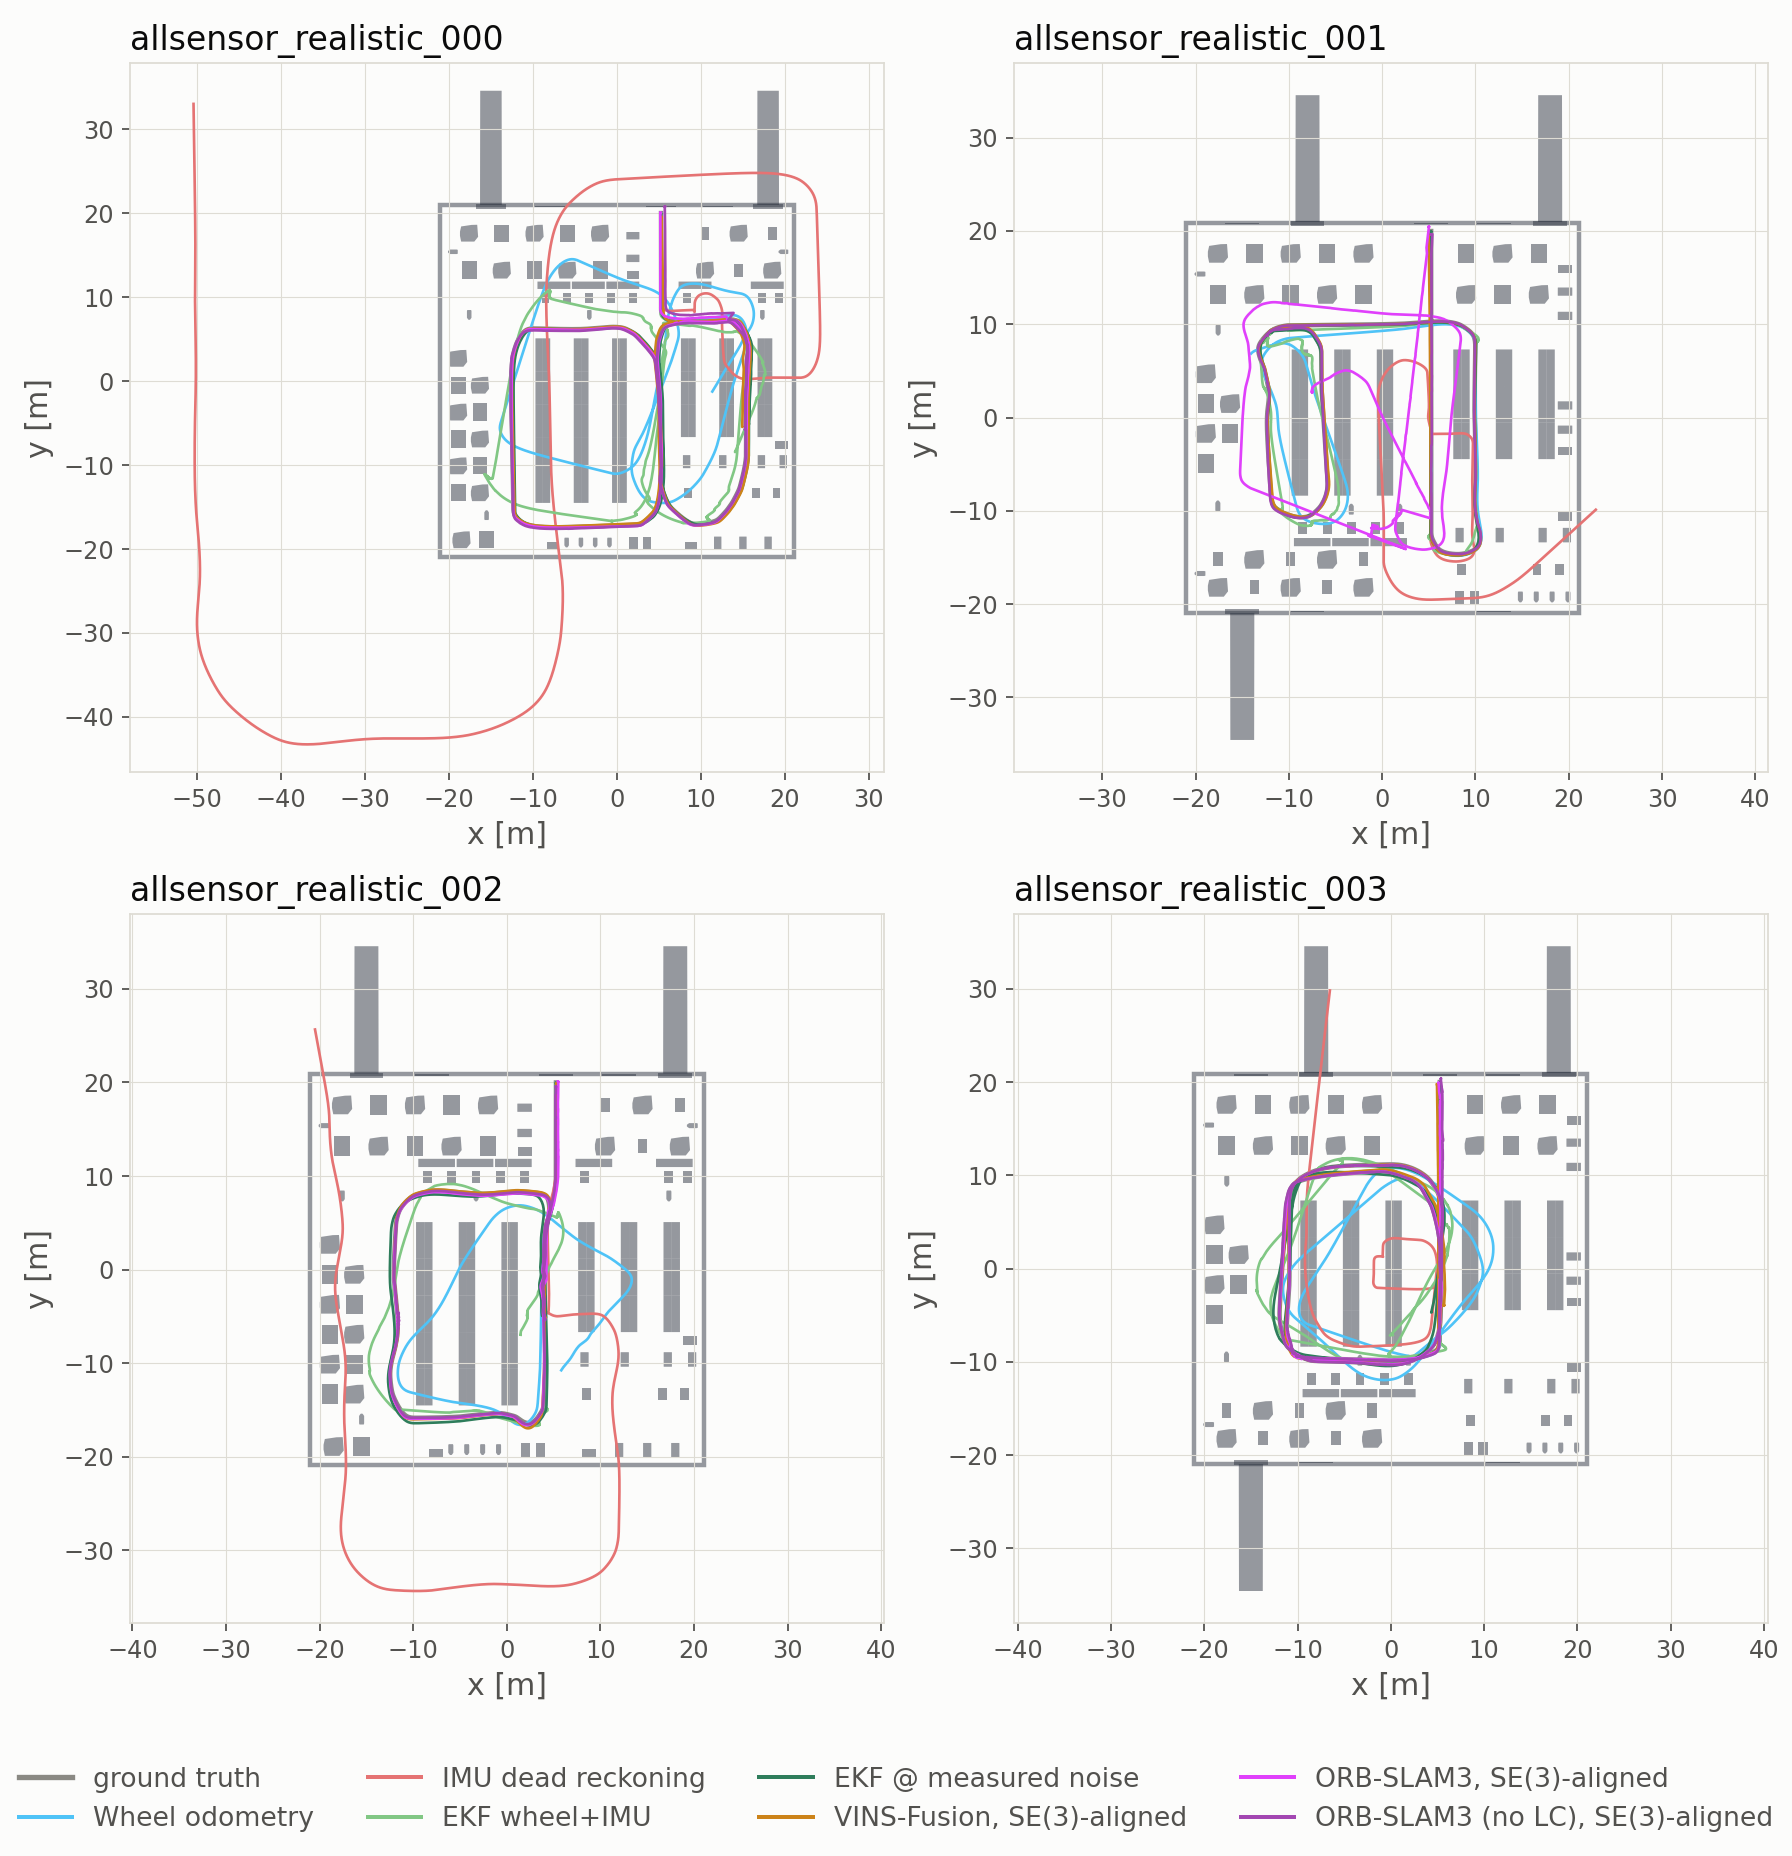
\includegraphics[width=0.96\textwidth]{figures/proprio_trajectories_grid_realistic.png}
  \caption[Estimator comparison on every realistic recording, world frame.]{
  Estimator comparison on every realistic recording, world frame: the
  dead-reckoning estimators as estimated from the ground-truth start pose,
  the visual estimators after the rigid $SE(3)$ alignment used for their
  metrics, one legend for all four panels. The IMU leaves the building on
  every recording; the EKF at the visual systems' noise (light green) wanders
  in heading where the measured-noise filter (dark green) stays on the route;
  ORB-SLAM3's divergent runs are the excursions on \repo{001} (loop closer
  active) and \repo{003} (closer disabled).}
  \label{fig:exp1-grid}
\end{figure}

\paragraph{Analysis.} With both families on the same hand-set inertial model
the ordering is settled: VINS-Fusion is the most accurate estimator on every
recording (\SIrange{0.22}{0.66}{\metre}) and the EKF, at
\SIrange{0.68}{2.80}{\metre}, is behind it on all four and behind the better
ORB-SLAM3 run on three. The measured-noise diagnostic puts the same filter at
\SIrange{0.21}{0.58}{\metre}, ahead of VINS-Fusion on three of four, so the
whole of the EKF's deficit is the noise model and none of it the
architecture --- the September control, reproduced on new recordings and
larger.

The mechanism is the one isolated in September. The configuration's
gyroscope density is five to seven times the measured value, which inflates
the heading process noise forty-fold; with the heading unobserved except
through the wheel yaw-rate residual, that residual steers the heading instead
of the bias, and yaw RMS rises from \SIrange{0.4}{5.7}{\degree} to
\SIrange{4.5}{28.0}{\degree}. On routes of 100 to \SI{170}{\metre} with
repeated turns that heading error is what the aligned ATE measures.

ORB-SLAM3's divergences are not a loop-closure effect. With the GPU front end
six of eight runs hold \SIrange{0.17}{0.52}{\metre} and two diverge, to
\SI{4.78}{\metre} with the closer active on \repo{realistic_001} and to
\SI{1.91}{\metre} with it disabled on \repo{realistic_003}, while the other
closer state on each of those recordings holds \SI{0.40}{} and
\SI{0.50}{\metre}. Each divergent run carries three or seven jumps
(\cref{tab:exp1-rpe}) and its clean relative error is as low as the stable
runs', so the error is a few discrete events, not steady-state tracking.
Which front-end condition produces them is not isolated here; the CPU runs of
the same recordings are scored below, where the same pattern recurs.

Traffic appears as a condition, not a tested factor. VINS-Fusion is
\SI{0.66}{\metre} on the U traffic recording against \SI{0.29}{\metre} on its
static twin and \SI{0.27}{\metre} against \SI{0.22}{\metre} on the I layout;
the proprioceptive estimators are unaffected by construction. The U recordings
do not share a route, so the difference cannot be credited to traffic alone.

The complementary failure of the two proprioceptive sensors holds. The IMU
keeps heading to \SIrange{0.5}{1.9}{\degree} RMS and loses position by
\SIrange{12}{23}{\metre}; the wheels keep position to \SIrange{1.0}{4.8}{\metre}
and lose \SIrange{7}{36}{\degree} of heading. Every proprioceptive covariance
is overconfident: ANEES \SIrange{8}{3399}{} against 3.0, the EKF at the
configuration noise least so because its inflated process noise is closer to
the error it actually makes.

\subsubsection{Visual estimators}

\paragraph{Results.} VINS-Fusion holds \SIrange{0.22}{0.66}{\metre} aligned
ATE on the four recordings with no jump and \SIrange{1.2}{3.6}{\degree} of
rotation error; its worst recording is the U layout with traffic,
\SI{0.66}{\metre} against \SI{0.29}{\metre} on that layout's static twin,
while on the I layout traffic changes nothing (\SI{0.27}{} against
\SI{0.22}{\metre}). ORB-SLAM3 spans \SIrange{0.14}{6.02}{\metre}: eleven of its
sixteen runs lie between \SI{0.14}{} and \SI{0.52}{\metre} and five diverge, and
which five is decided by the loop closer and the recording, not by the front
end (\cref{tab:realistic-baseline}, \cref{fig:realistic-traj,fig:realistic-metrics}).
Neither front end loses tracking on any recording, with or without traffic:
zero tracking-loss events and zero resets in twenty runs.

Two columns of \cref{tab:realistic-baseline} qualify those RMSE figures. The
first is the worst single error each run reaches after its initialisation
transient, which the RMSE averages away: over the fifteen runs that held it is
\SIrange{0.26}{1.25}{\metre}, between \num{0.8} and \num{2.6} times the run's
own RMSE, so no run that tracked was ever more than about
\SI{1.25}{\metre} from the truth; over the five that diverged it is
\SIrange{2.25}{13.42}{\metre}. The two orderings are not the same one. On
\repo{realistic_000} VINS-Fusion has the lower RMSE
(\SI{0.290}{} against \SI{0.338}{\metre}) and ORB-SLAM3 the smaller worst
case (\SI{0.260}{} against \SI{0.576}{\metre}), so which estimator is
``better'' on that recording depends on whether the question is average
accuracy or the largest excursion --- and for a vehicle in a \SI{3.0}{\metre}
aisle it is the second. The exclusion matters: every ORB-SLAM3 run peaks near
\SI{2.5}{\second} at three to four metres on the gravity re-alignment that
ends its inertial initialisation, and a raw maximum would report that
initialisation as though it were driving.

The second column is the same ATE as a percentage of the ground-truth path
length. It exists so that these \SIrange{103}{172}{\metre} routes can be set
beside the real robot's much shorter ones,
and it separates the two outcomes more sharply than
the metre figure does: \SIrange{0.09}{0.64}{\percent} for the fifteen runs
that held against \SIrange{1.11}{4.51}{\percent} for the five that diverged.
It is a ratio of two quantities already in the table, not a KITTI-style
sub-sequence drift rate, and it is not comparable to one.

\reporttable{realistic_baseline_table}

\begin{figure}[p]
  \centering
  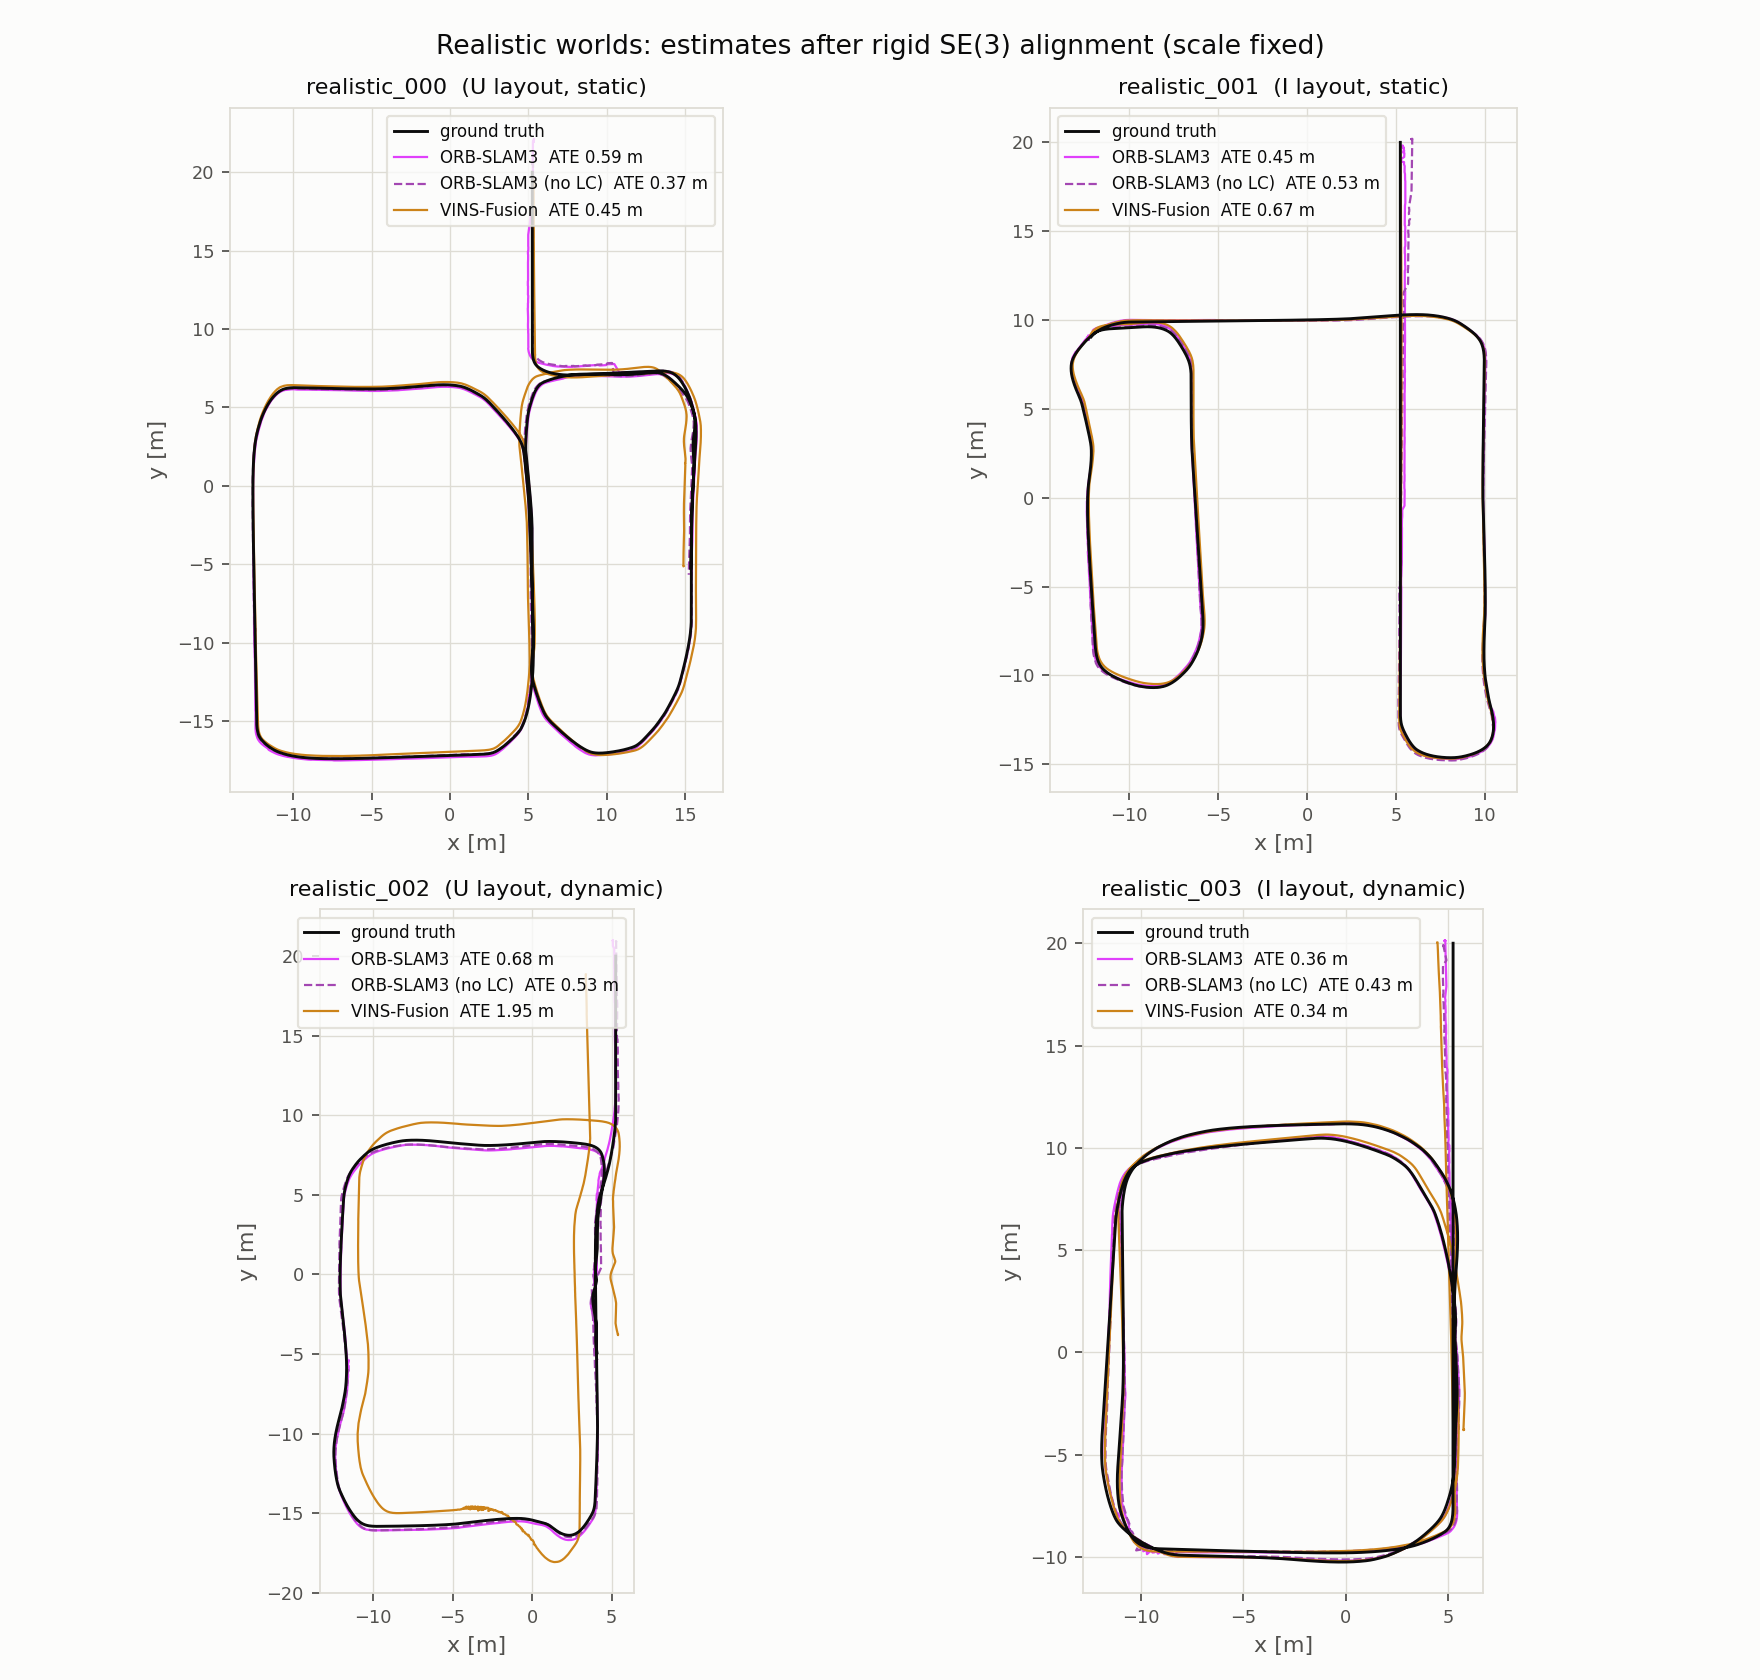
\includegraphics[width=0.92\textwidth]{figures/realistic_trajectories.png}
  \caption[Visual estimates on the four realistic recordings.]{Unfiltered
  estimates on the four realistic-warehouse recordings
  after rigid $SE(3)$ alignment with scale fixed, on the warehouse footprint.
  Top: the static twins; bottom: the same layouts with traffic. Solid magenta
  is ORB-SLAM3 with its loop closer active, dashed with it disabled, lighter
  for the GPU front end; orange is VINS-Fusion. The two excursions on
  \repo{realistic_001} are the loop-closing runs after their false closure;
  the \SI{1.4}{\metre} run on \repo{realistic_002} is the CPU loop-closing
  run; the closure-free runs on \repo{realistic_003} lie on the route in plan
  and diverge vertically.}
  \label{fig:realistic-traj}
\end{figure}

\begin{figure}[htbp]
  \centering
  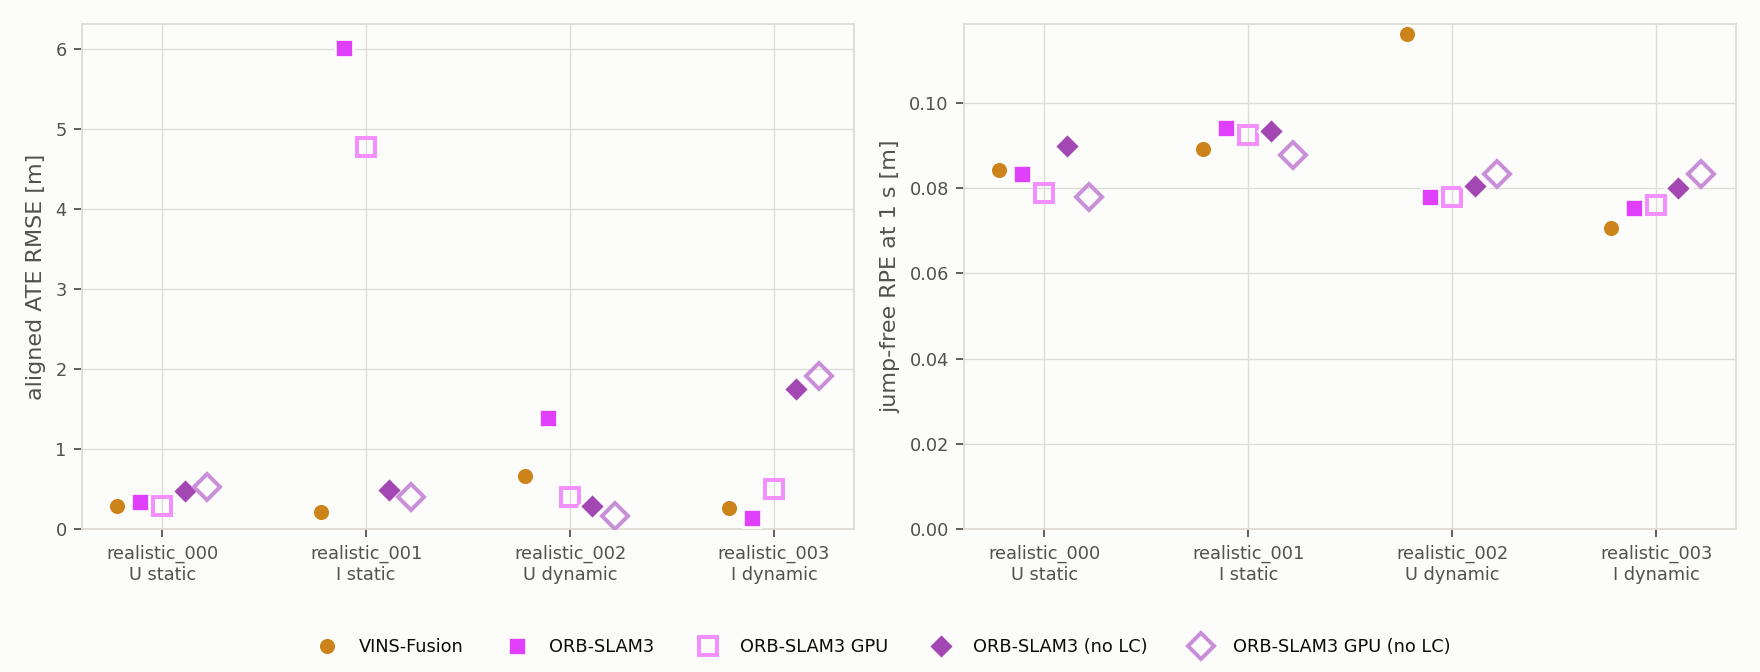
\includegraphics[width=\textwidth]{figures/realistic_metrics.png}
  \caption[Aligned ATE and jump-free RPE of the visual arms.]{Aligned ATE
  (left) and jump-free translational RPE at
  \SI{1}{\second} (right) of every visual run, one marker per run; filled
  markers are the CPU front end, open markers the GPU front end of the same
  configuration. The relative error is \SIrange{0.07}{0.12}{\metre} for every
  run, so the ATE differences are discrete events, not tracking quality.}
  \label{fig:realistic-metrics}
\end{figure}

\paragraph{Analysis: the loop closer decides, in both directions.} On the
static I layout both loop-closing runs accept one closure at \SI{73.2}{\second},
in the heading change at \SI{76}{\percent} of the route, with a correction of
\SI{14.7}{\metre} (CPU) and \SI{13.3}{\metre} (GPU) and \SIrange{1.9}{2.8}{\degree};
a global bundle adjustment follows and the trajectory is \SI{6.02}{} and
\SI{4.78}{\metre} off for the rest of the run, where the two closure-free runs
on the same recording hold \SI{0.50}{} and \SI{0.40}{\metre}
(\cref{fig:tl-real-001}). A route with half a metre of accumulated error
cannot need a fourteen-metre correction, so the match is false: the I layout's
long parallel aisles present the same rack faces twice, and the matched
keyframes (97 against 255, 104 against 272) are one aisle apart. The same
candidate was then re-proposed four times and rejected by the inertial
geometry check, after the damage. That both front ends accept it at the same
frame with the same correction says the place-recognition stage, not the
extractor, is where the fault lies.

On the I layout with traffic the sign reverses. Both loop-closing runs accept
one closure at \SI{56.5}{\second} (\SI{48}{\percent} of the route) with a
\SI{0.33}{\metre} correction and hold \SI{0.14}{} and \SI{0.50}{\metre}; the
closure-free runs read \SI{1.76}{} and \SI{1.91}{\metre}, yet their planar
error never exceeds \SI{0.7}{\metre} (\cref{fig:tl-real-003}). The difference
is vertical: the closure-free estimates climb to \SI{4.7}{} and
\SI{5.1}{\metre} above the floor by the end of the run while the loop-closing
runs stay within \SI{0.6}{} and \SI{1.4}{\metre}, and the three-dimensional
ATE reports that climb. The GPU loop-closing run on this recording also
rejected 148 further candidates by inertial geometry, every one of them after
its single accepted closure. On the U layout the closer is nearly inert: two
accepted closures per run on \repo{realistic_000} with corrections of
\SIrange{0.07}{0.12}{\metre}, one of \SIrange{0.26}{0.33}{\metre} per run on
\repo{realistic_002}, and the eight U-layout ORB-SLAM3 runs within
\SIrange{0.17}{0.52}{\metre} except the CPU loop-closing run on
\repo{realistic_002}, whose \SI{1.39}{\metre} is an offset present from
\SI{6.5}{\second} on, before any closure (\cref{fig:tl-real-002}); with four
jumps and the lowest relative error on the recording it is an initialisation
event, not a tracking one, and the GPU run of the same configuration, which
accepts the same closure at \SI{65}{\second}, does not reproduce it
(\SI{0.40}{\metre}).

\paragraph{Analysis: the front end changes throughput, not accuracy.} The GPU
extractor processes \SIrange{97}{99}{\percent} of each bag's frames where the
CPU extractor processes \SIrange{72}{94}{\percent}, and its tracking median
is \SIrange{30}{37}{\milli\second} against \SIrange{49}{55}{\milli\second}
(from the per-run \repo{performance.csv}). Across the eight CPU/GPU pairs
with the same closer state the ATE differs by at most \SI{0.16}{\metre} in
five; the three larger differences (\SI{-1.2}{}, \SI{-1.0}{} and
\SI{+0.4}{\metre}) are each one run's discrete event, in both directions,
and the two divergence patterns above occur in both front ends alike. At this frame budget the extractor is not the limiting
stage of accuracy on these recordings.

\paragraph{Analysis: traffic as a condition.} VINS-Fusion is \SI{0.37}{\metre}
worse on the U layout with traffic than on its static twin and \SI{0.05}{\metre}
worse on the I layout; its relative error on \repo{realistic_002} is the
highest of any run (\SI{0.116}{\metre}) and its error trace carries two
waves of \SI{0.7}{\metre} at \SI{25}{} and \SI{45}{\second} on the western and
southern aisles, where the pallet jacks work, that no static run shows
(\cref{fig:tl-real-002}). ORB-SLAM3's closure-free runs are \emph{better} on
the U traffic recording (\SI{0.29}{}, \SI{0.17}{\metre}) than on its static
twin (\SI{0.48}{}, \SI{0.52}{\metre}). With one run per cell and routes that
differ between twin and traffic recording, neither number is a traffic effect;
what the slot establishes is that physically simulated traffic degrades the
tracker that follows features longest, and breaks neither.

\paragraph{Analysis: the two estimators err in perpendicular directions.}
VINS-Fusion drifts sideways and ORB-SLAM3 drifts forwards, which the aligned
ATE cannot show. Decomposing each run's error in the ground-truth heading frame
(\reporttable{exp1_translation_pattern}, \cref{fig:exp1-translation-pattern}),
VINS-Fusion's cross-track share of the planar error is
\numrange{0.67}{0.73} on three of the four recordings while every ORB-SLAM3 run
that held tracking lies between \num{0.11} and \num{0.25}. On
\repo{realistic_000} the two score \SI{0.293}{} and \SI{0.290}{\metre}:
indistinguishable, and perpendicular. For a \num{0.83} by \SI{0.50}{\metre}
robot in a \SI{3.0}{\metre} aisle they are not equally safe, because
cross-track error closes the gap to the racking and along-track error does not.

The false closure is also the failure that throws the estimate sideways. The
two loop-closing runs on \repo{realistic_001} are the only ORB-SLAM3 runs whose
cross-track share exceeds \num{0.5} (\num{0.62} and \num{0.69}), with
cross-track RMS of \SI{4.76}{} and \SI{3.98}{\metre}; of the five diverged runs
only those two are cross-track dominated, so the direction belongs to the false
closure and not to divergence in general. The error is scatter rather than
offset throughout: the mean of each signed component is
\numrange{0.17}{0.36} of its RMS in every arm. Both decompositions are computed
on the same aligned series the reported ATE uses, so the parts account for the
whole, and both are pooled over the twenty runs rather than ranked, because one
run per cell cannot separate arms that differ by less than ORB-SLAM3's
\SI{0.277}{\metre} run-to-run spread.

\paragraph{Analysis: the rotation column.} ORB-SLAM3's \SIrange{13}{19}{\degree}
rotational RMSE is one event on every run: the first jump lies at
\SIrange{2.5}{4.8}{\second} (\cref{tab:realistic-timelines-baseline}), where
inertial initialisation re-aligns the world frame to gravity, and after it the
clean rotational RPE is \SIrange{0.07}{0.33}{\degree}. The jump detector is
translational, so the column includes the event; the median is the number to
read. Splitting the error by axis confirms what kind of event it is
(\reporttable{exp1_rotation_pattern}, \cref{fig:exp1-rotation-pattern}): yaw,
pitch and roll RMS are all \SIrange{14}{19}{\degree} while their medians are
\SIrange{0.88}{1.51}{\degree}, and an error that moves all three axes together
and persists in none is a frame re-alignment rather than drift. Turning does
not raise the rotation error either: pooled over the twenty runs the median
while turning exceeds the median while straight by \SI{+0.01}{\degree}, and
eleven of twenty runs are positive, which is a coin flip. VINS-Fusion carries a
smaller signature of the same kind, pitch and roll RMS of \SI{1.05}{} and
\SI{1.33}{\degree} against a yaw RMS of \SI{0.24}{\degree};
\flag{whether that is a residual gravity error or the rigid fit absorbing a
tilt has not been separated, and it is reported as an observation.}

\reporttable{realistic_baseline_timeline}

\begin{figure}[p]
  \centering
  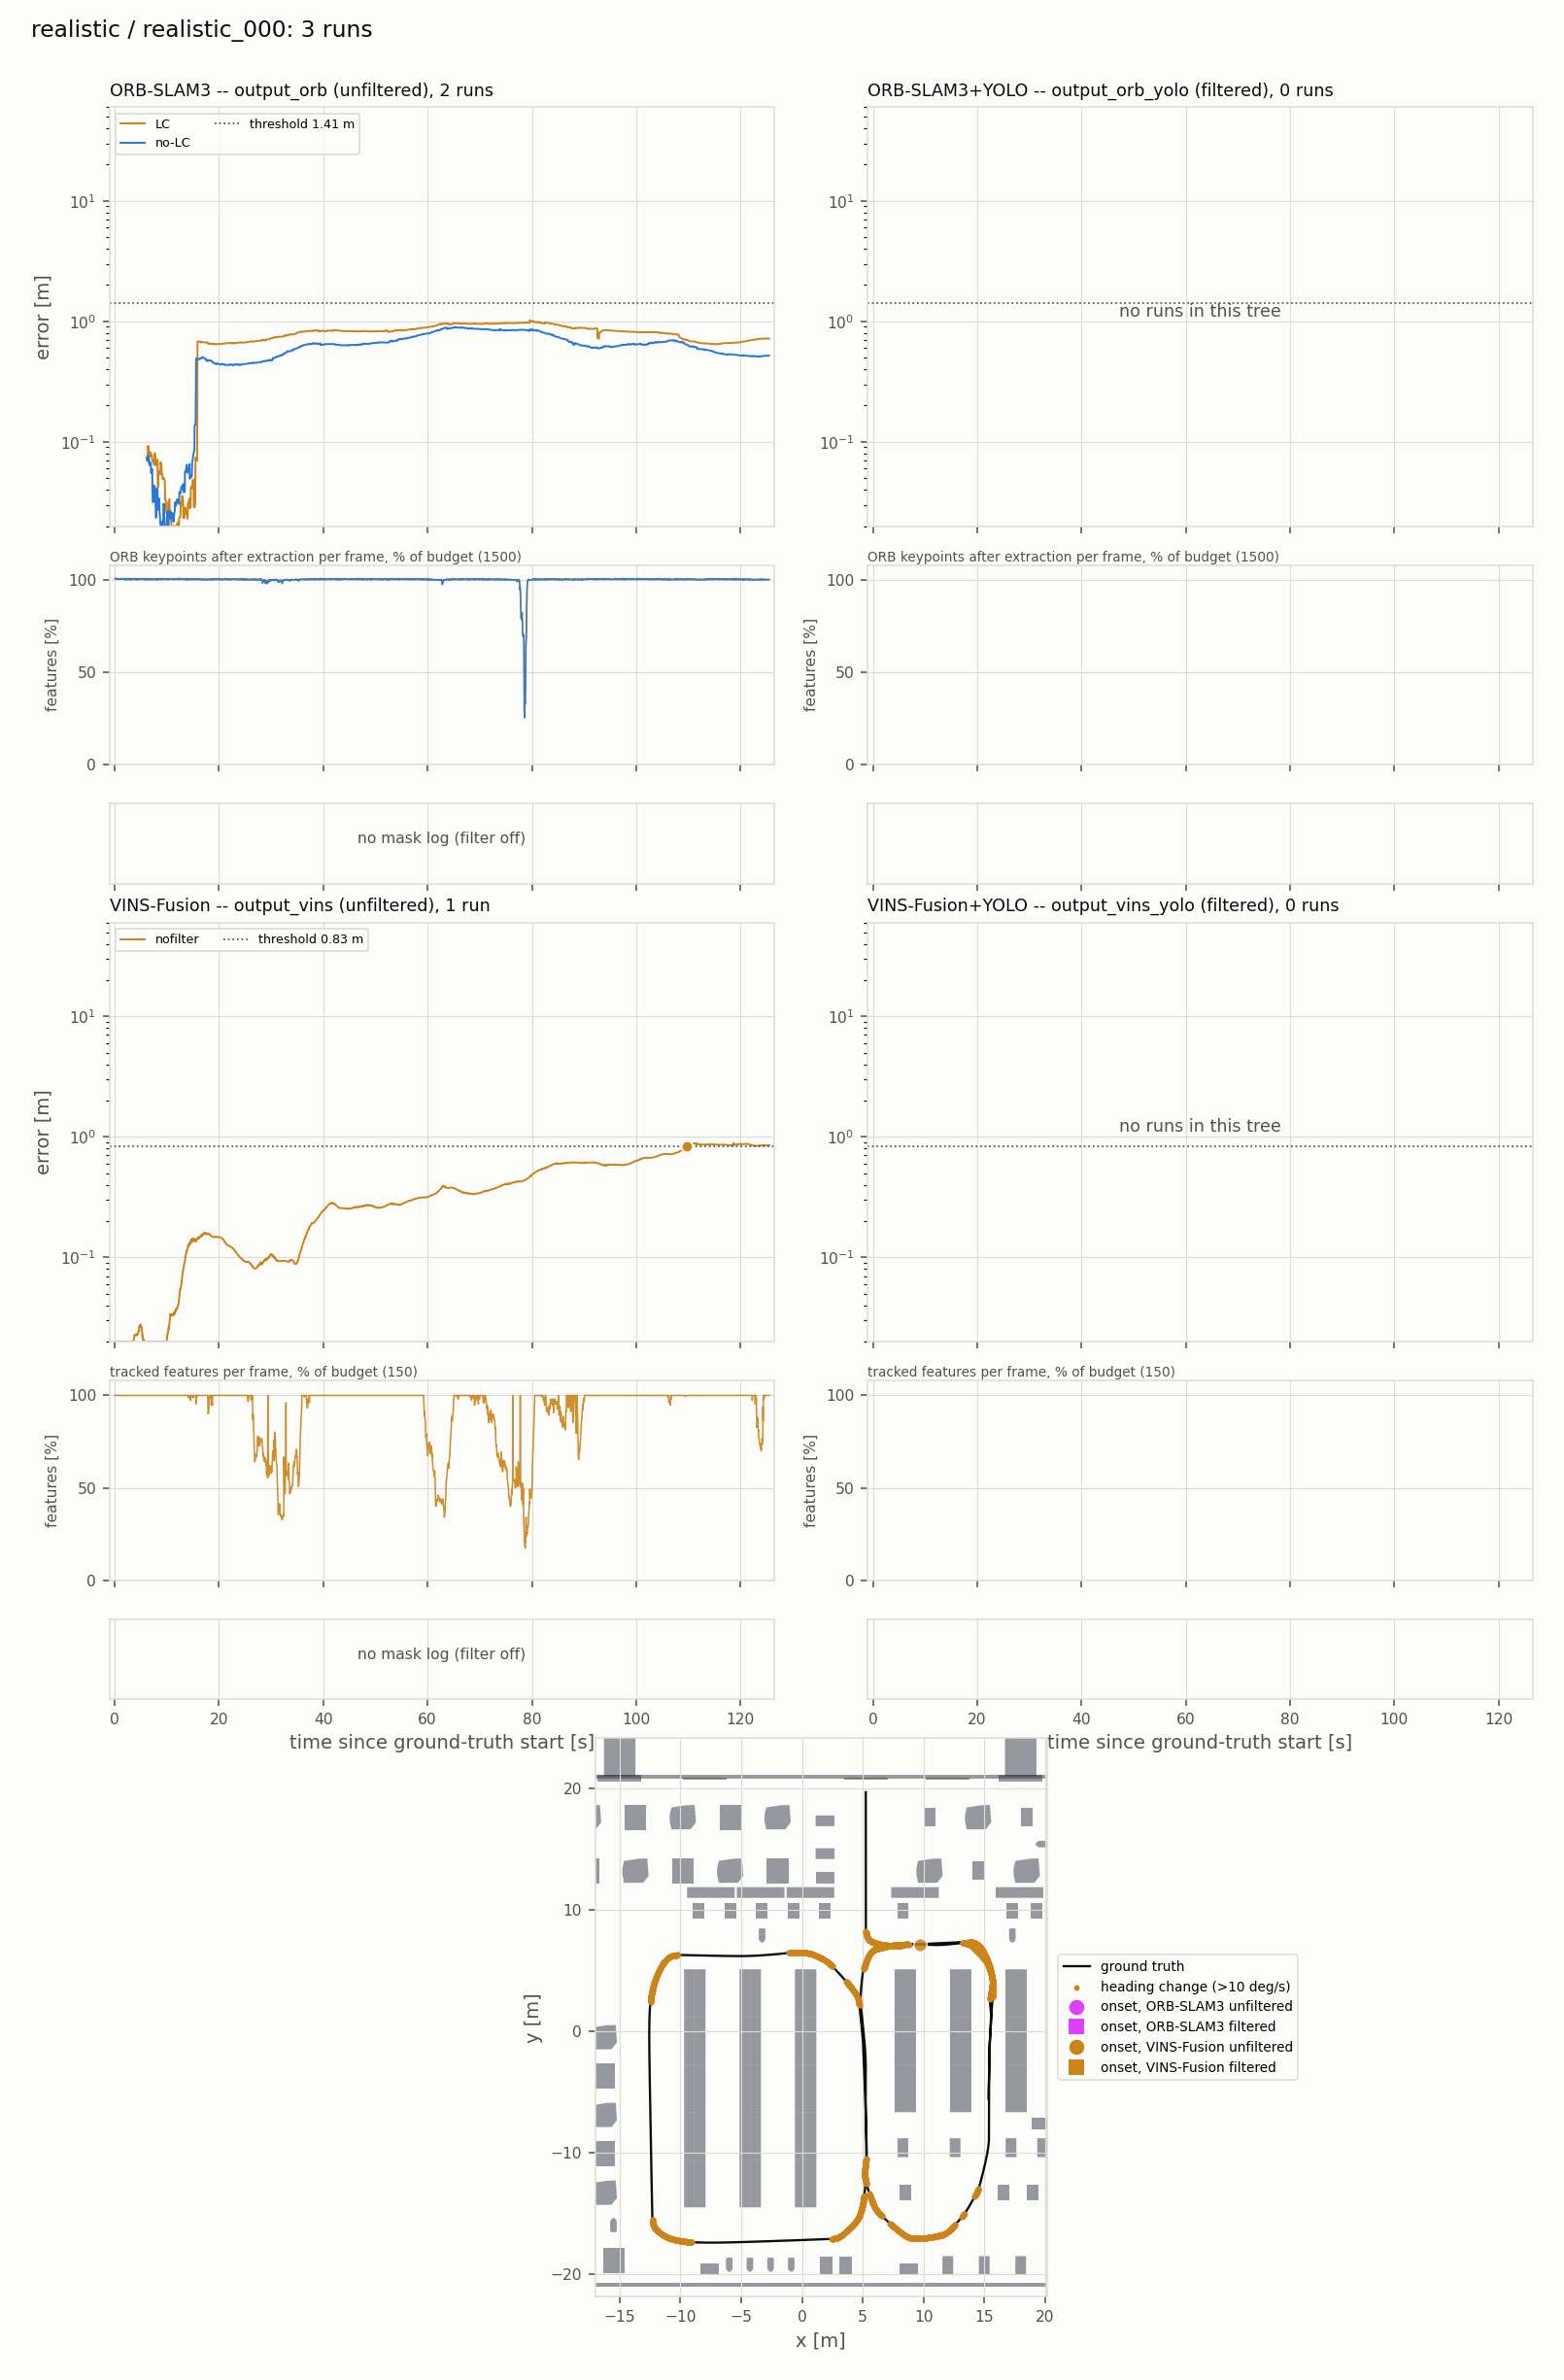
\includegraphics[width=0.98\textwidth]{figures/timeline_realistic__realistic_000.png}
  \caption[Timelines, static U-layout recording.]{\repo{realistic_000} (U,
  static), every run. Left: start-anchored
  planar error on a log axis, solid for loop closing active, dotted for
  disabled, lighter for the GPU front end, with each estimator's threshold;
  the dot marks the onset of sustained excess. Right: the route with heading
  changes in orange and every onset placed on it. The one onset is the GPU
  closure-free run at \SI{60}{\second}, a sustained \SI{1.3}{\metre} offset on
  the straight, not a jump.}
  \label{fig:tl-real-000}
\end{figure}
\begin{figure}[p]
  \centering
  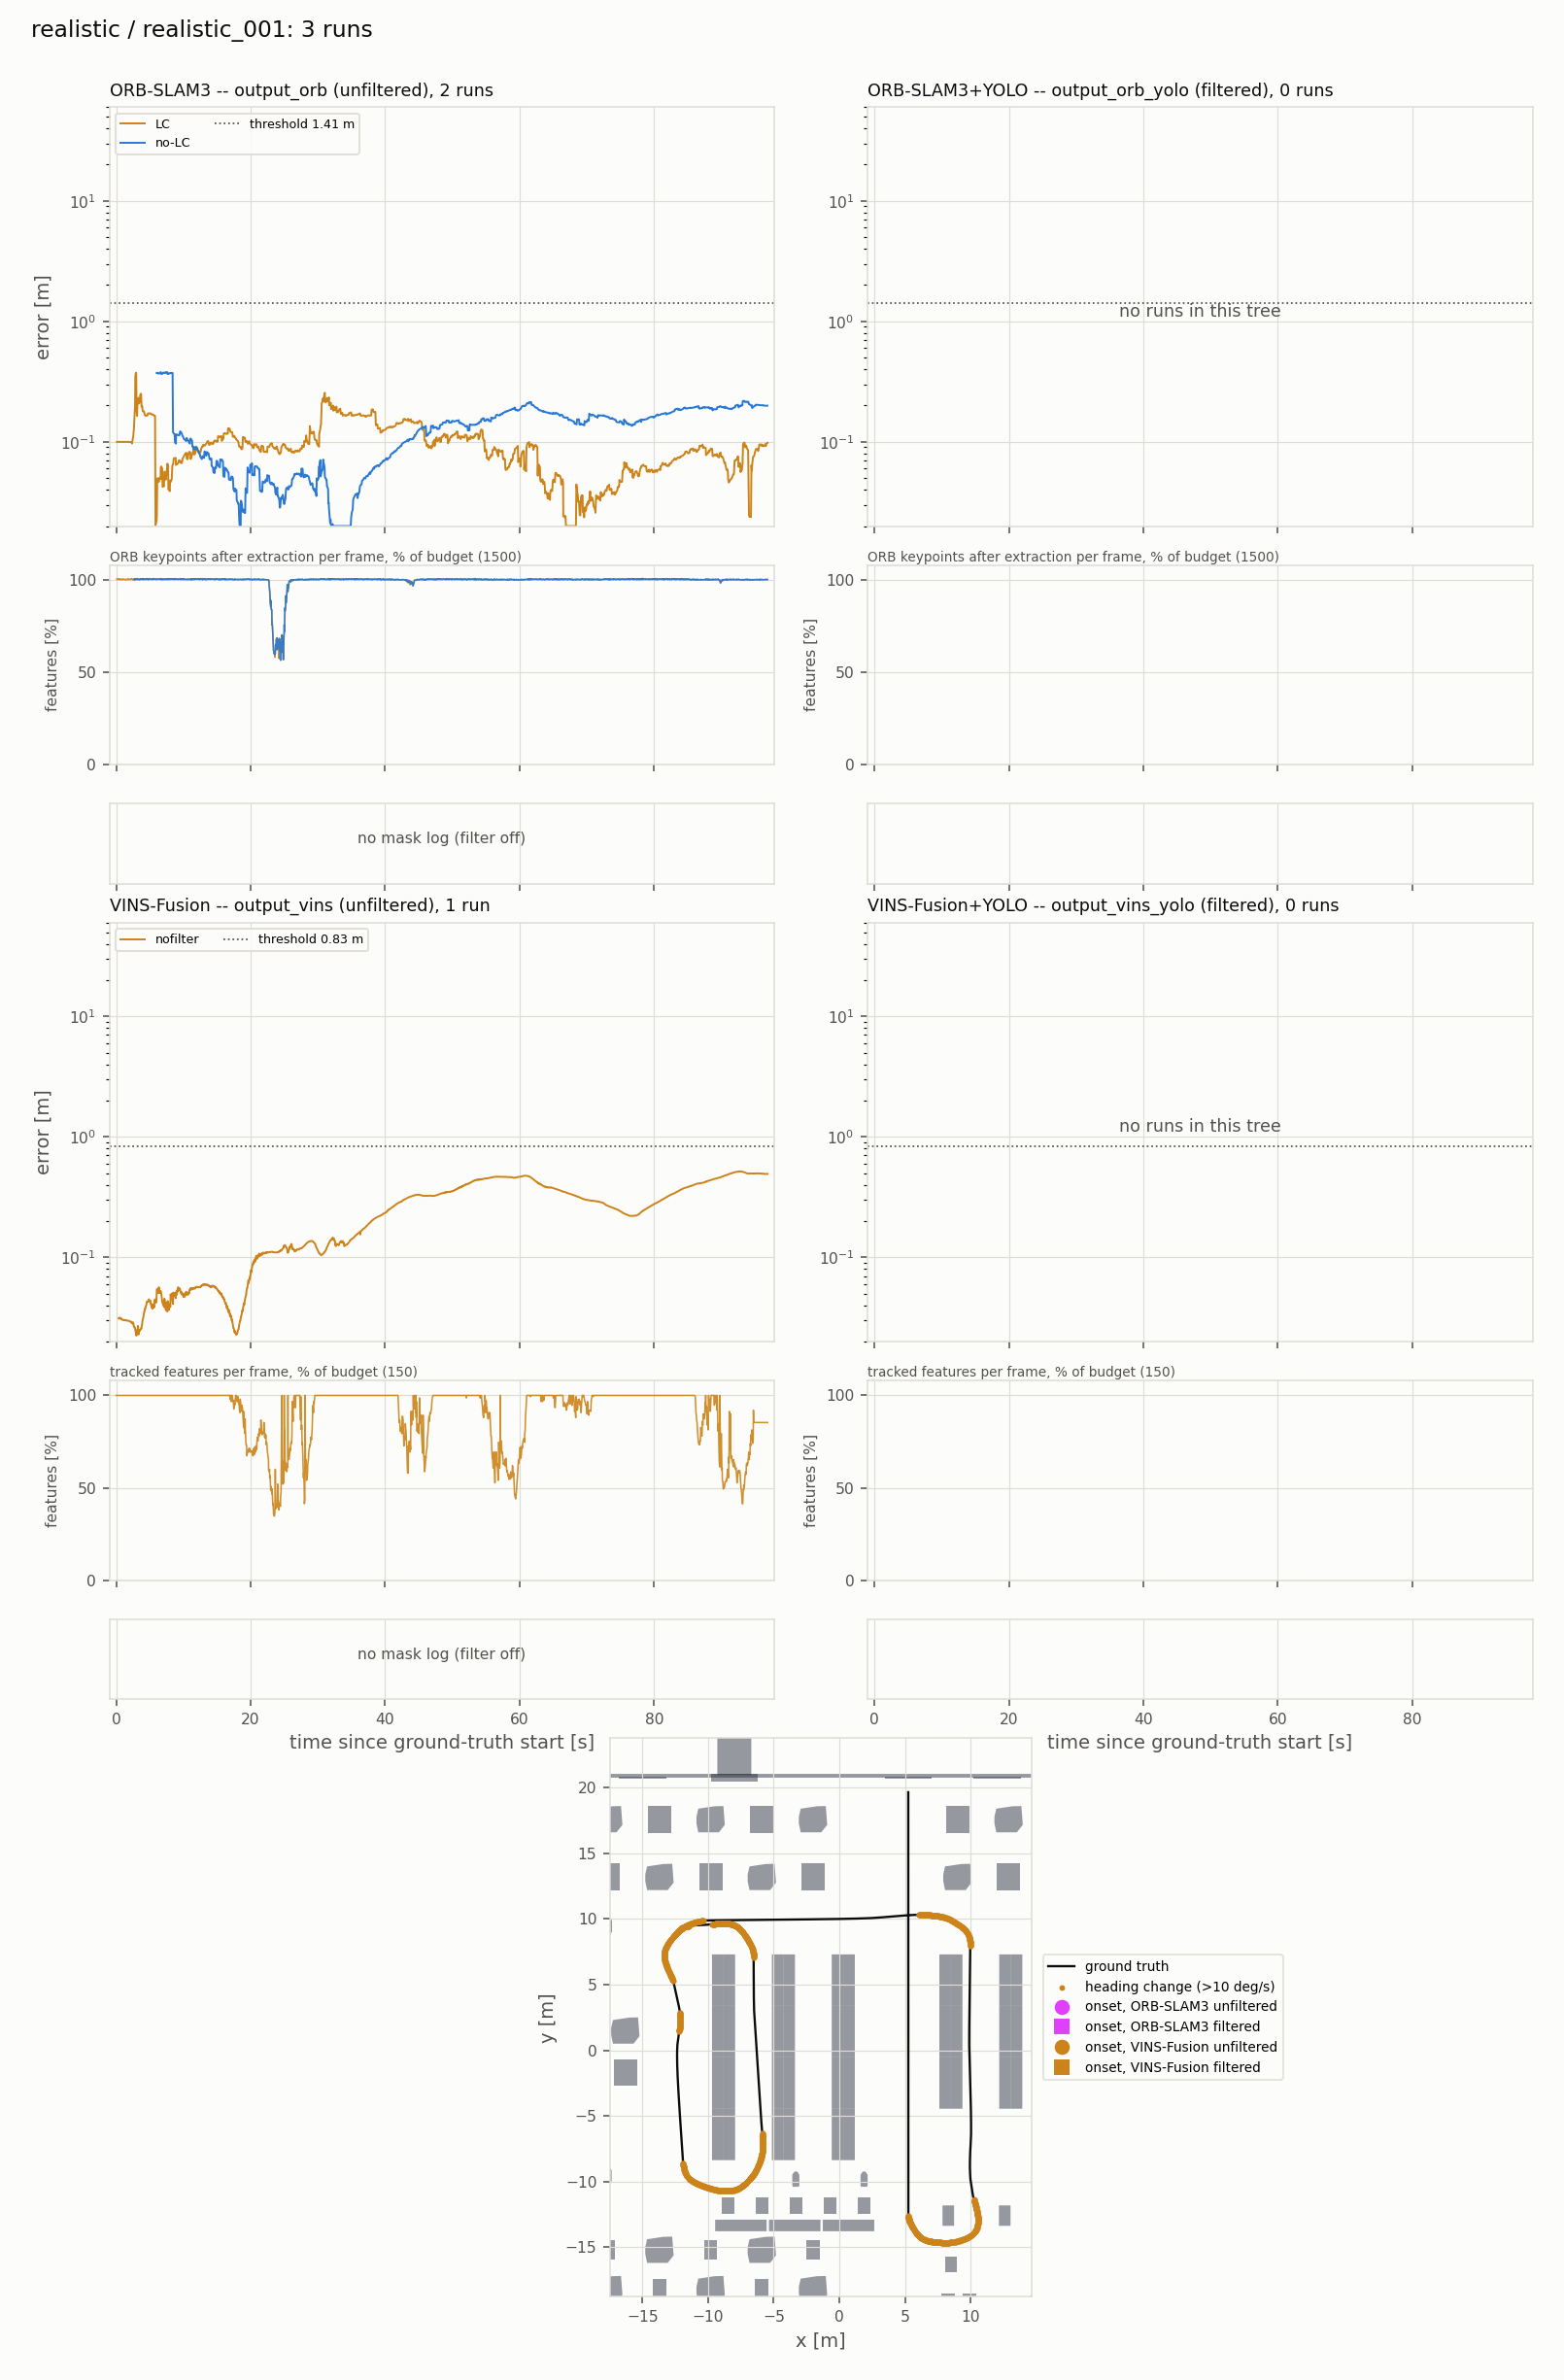
\includegraphics[width=0.98\textwidth]{figures/timeline_realistic__realistic_001.png}
  \caption[Timelines, static I-layout recording.]{\repo{realistic_001} (I,
  static), every run; panels as in
  \cref{fig:tl-real-000}. Both loop-closing runs step to \SI{14}{\metre} of
  error at \SI{73}{\second}, in the heading change at \SI{76}{\percent} of the
  route, at the single accepted closure; the closure-free runs and VINS-Fusion
  never cross.}
  \label{fig:tl-real-001}
\end{figure}
\begin{figure}[p]
  \centering
  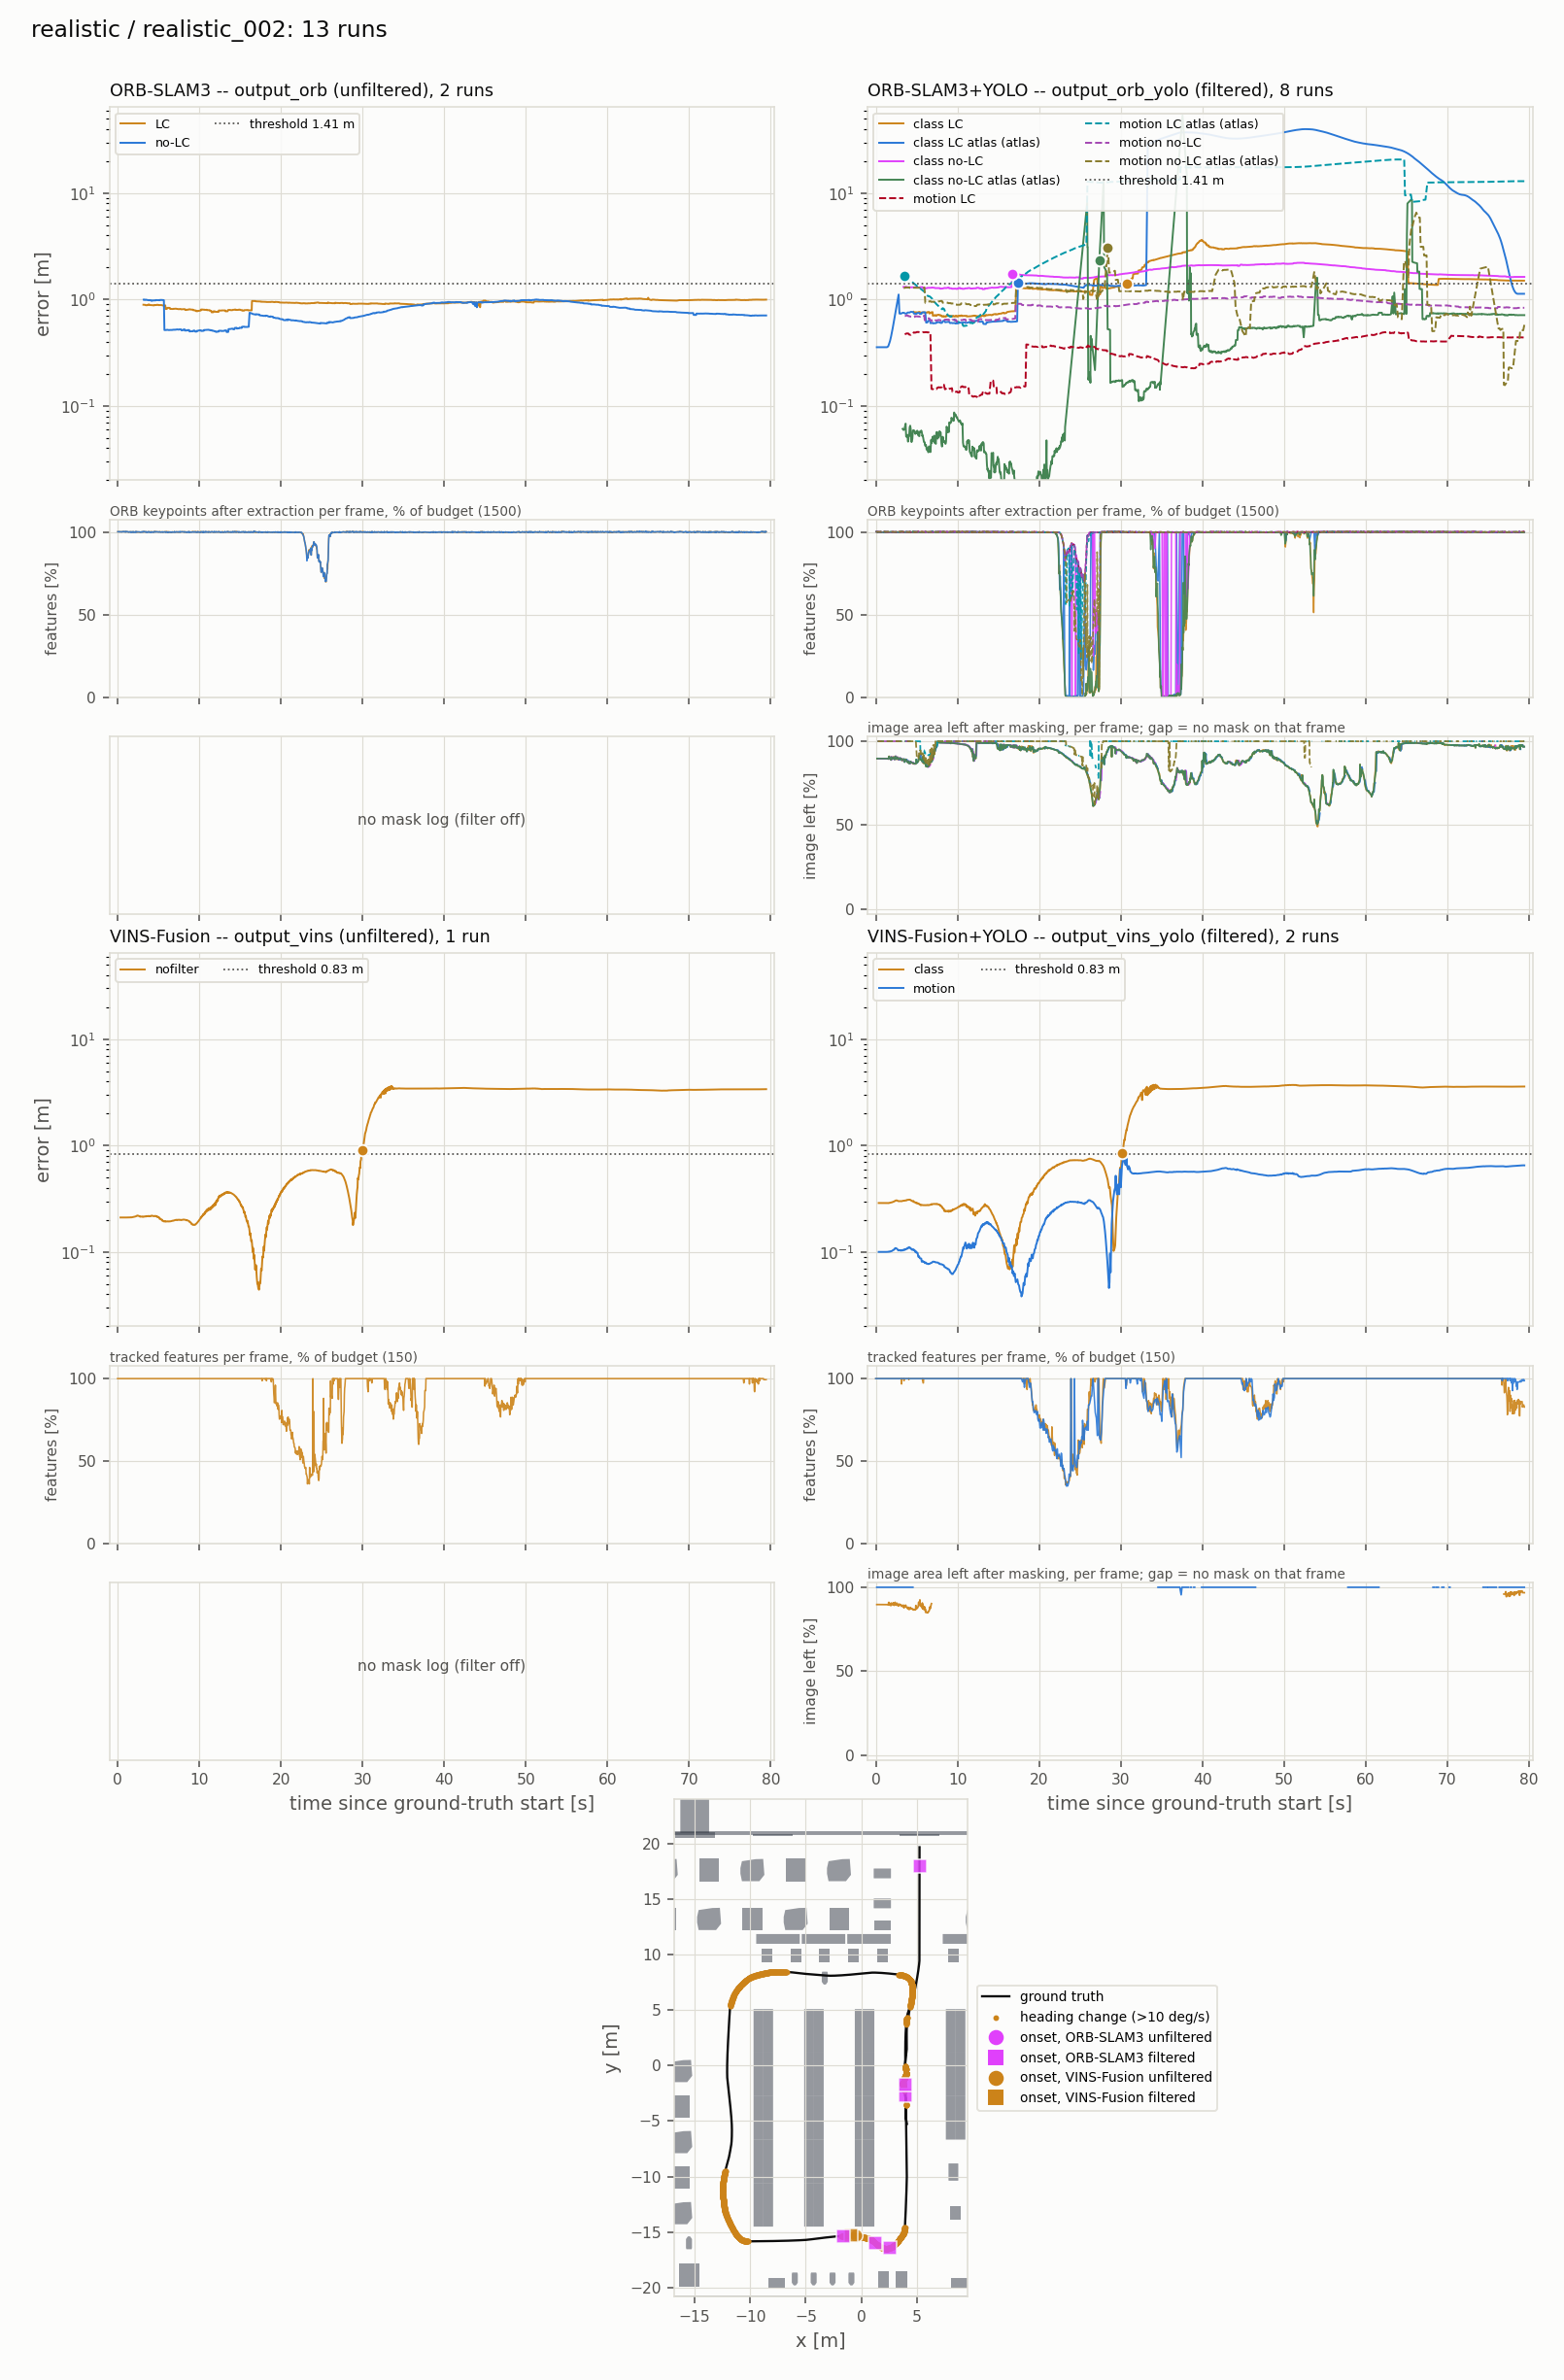
\includegraphics[width=0.98\textwidth]{figures/timeline_realistic__realistic_002.png}
  \caption[Timelines, U-layout recording with traffic.]{\repo{realistic_002}
  (U, traffic), every run; panels as in
  \cref{fig:tl-real-000}. The CPU loop-closing run carries a \SI{1.5}{\metre}
  offset from \SI{6.5}{\second}, which the GPU loop-closing run does not
  share; VINS-Fusion's two \SI{0.7}{\metre} waves at \SI{25}{} and
  \SI{45}{\second} lie on the aisles where the pallet jacks work.}
  \label{fig:tl-real-002}
\end{figure}
\begin{figure}[p]
  \centering
  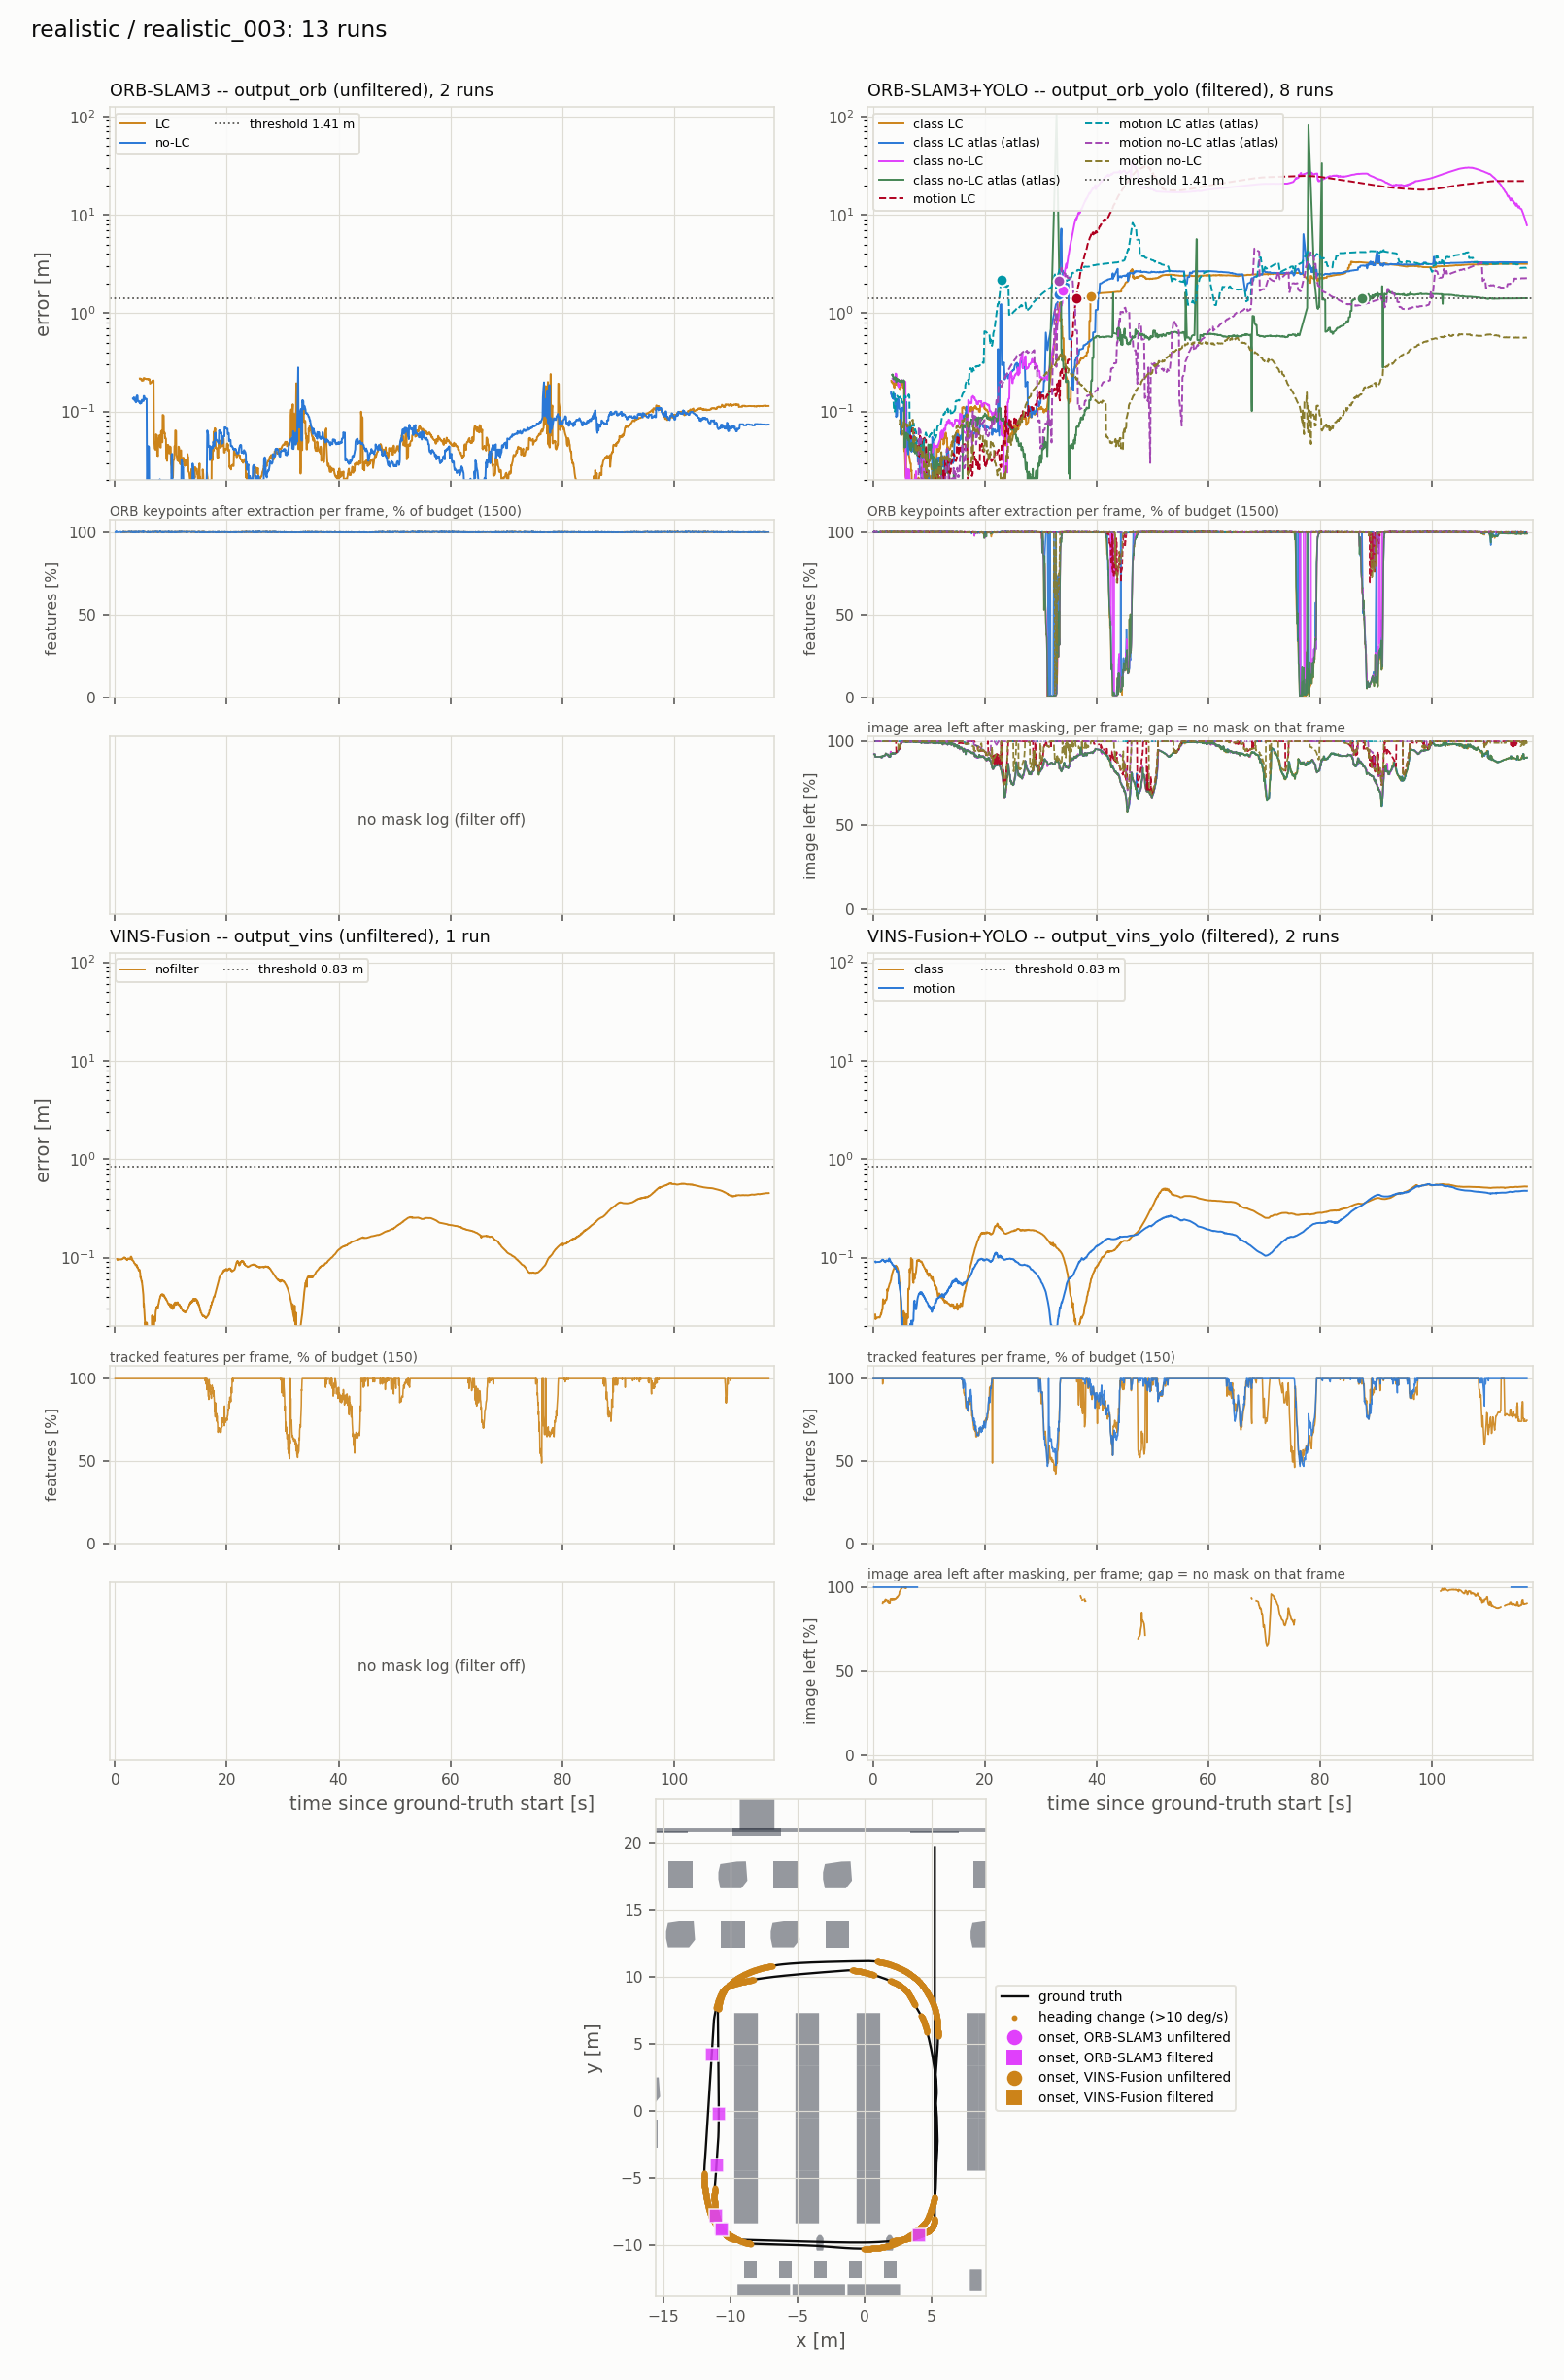
\includegraphics[width=0.98\textwidth]{figures/timeline_realistic__realistic_003.png}
  \caption[Timelines, I-layout recording with traffic.]{\repo{realistic_003}
  (I, traffic), every run; panels as in
  \cref{fig:tl-real-000}. No run crosses its threshold in the plane; the
  \SI{1.8}{} and \SI{1.9}{\metre} ATE of the closure-free runs is vertical
  drift, which the single accepted closure of the loop-closing runs removes.}
  \label{fig:tl-real-003}
\end{figure}

\begin{figure}[p]
  \centering
  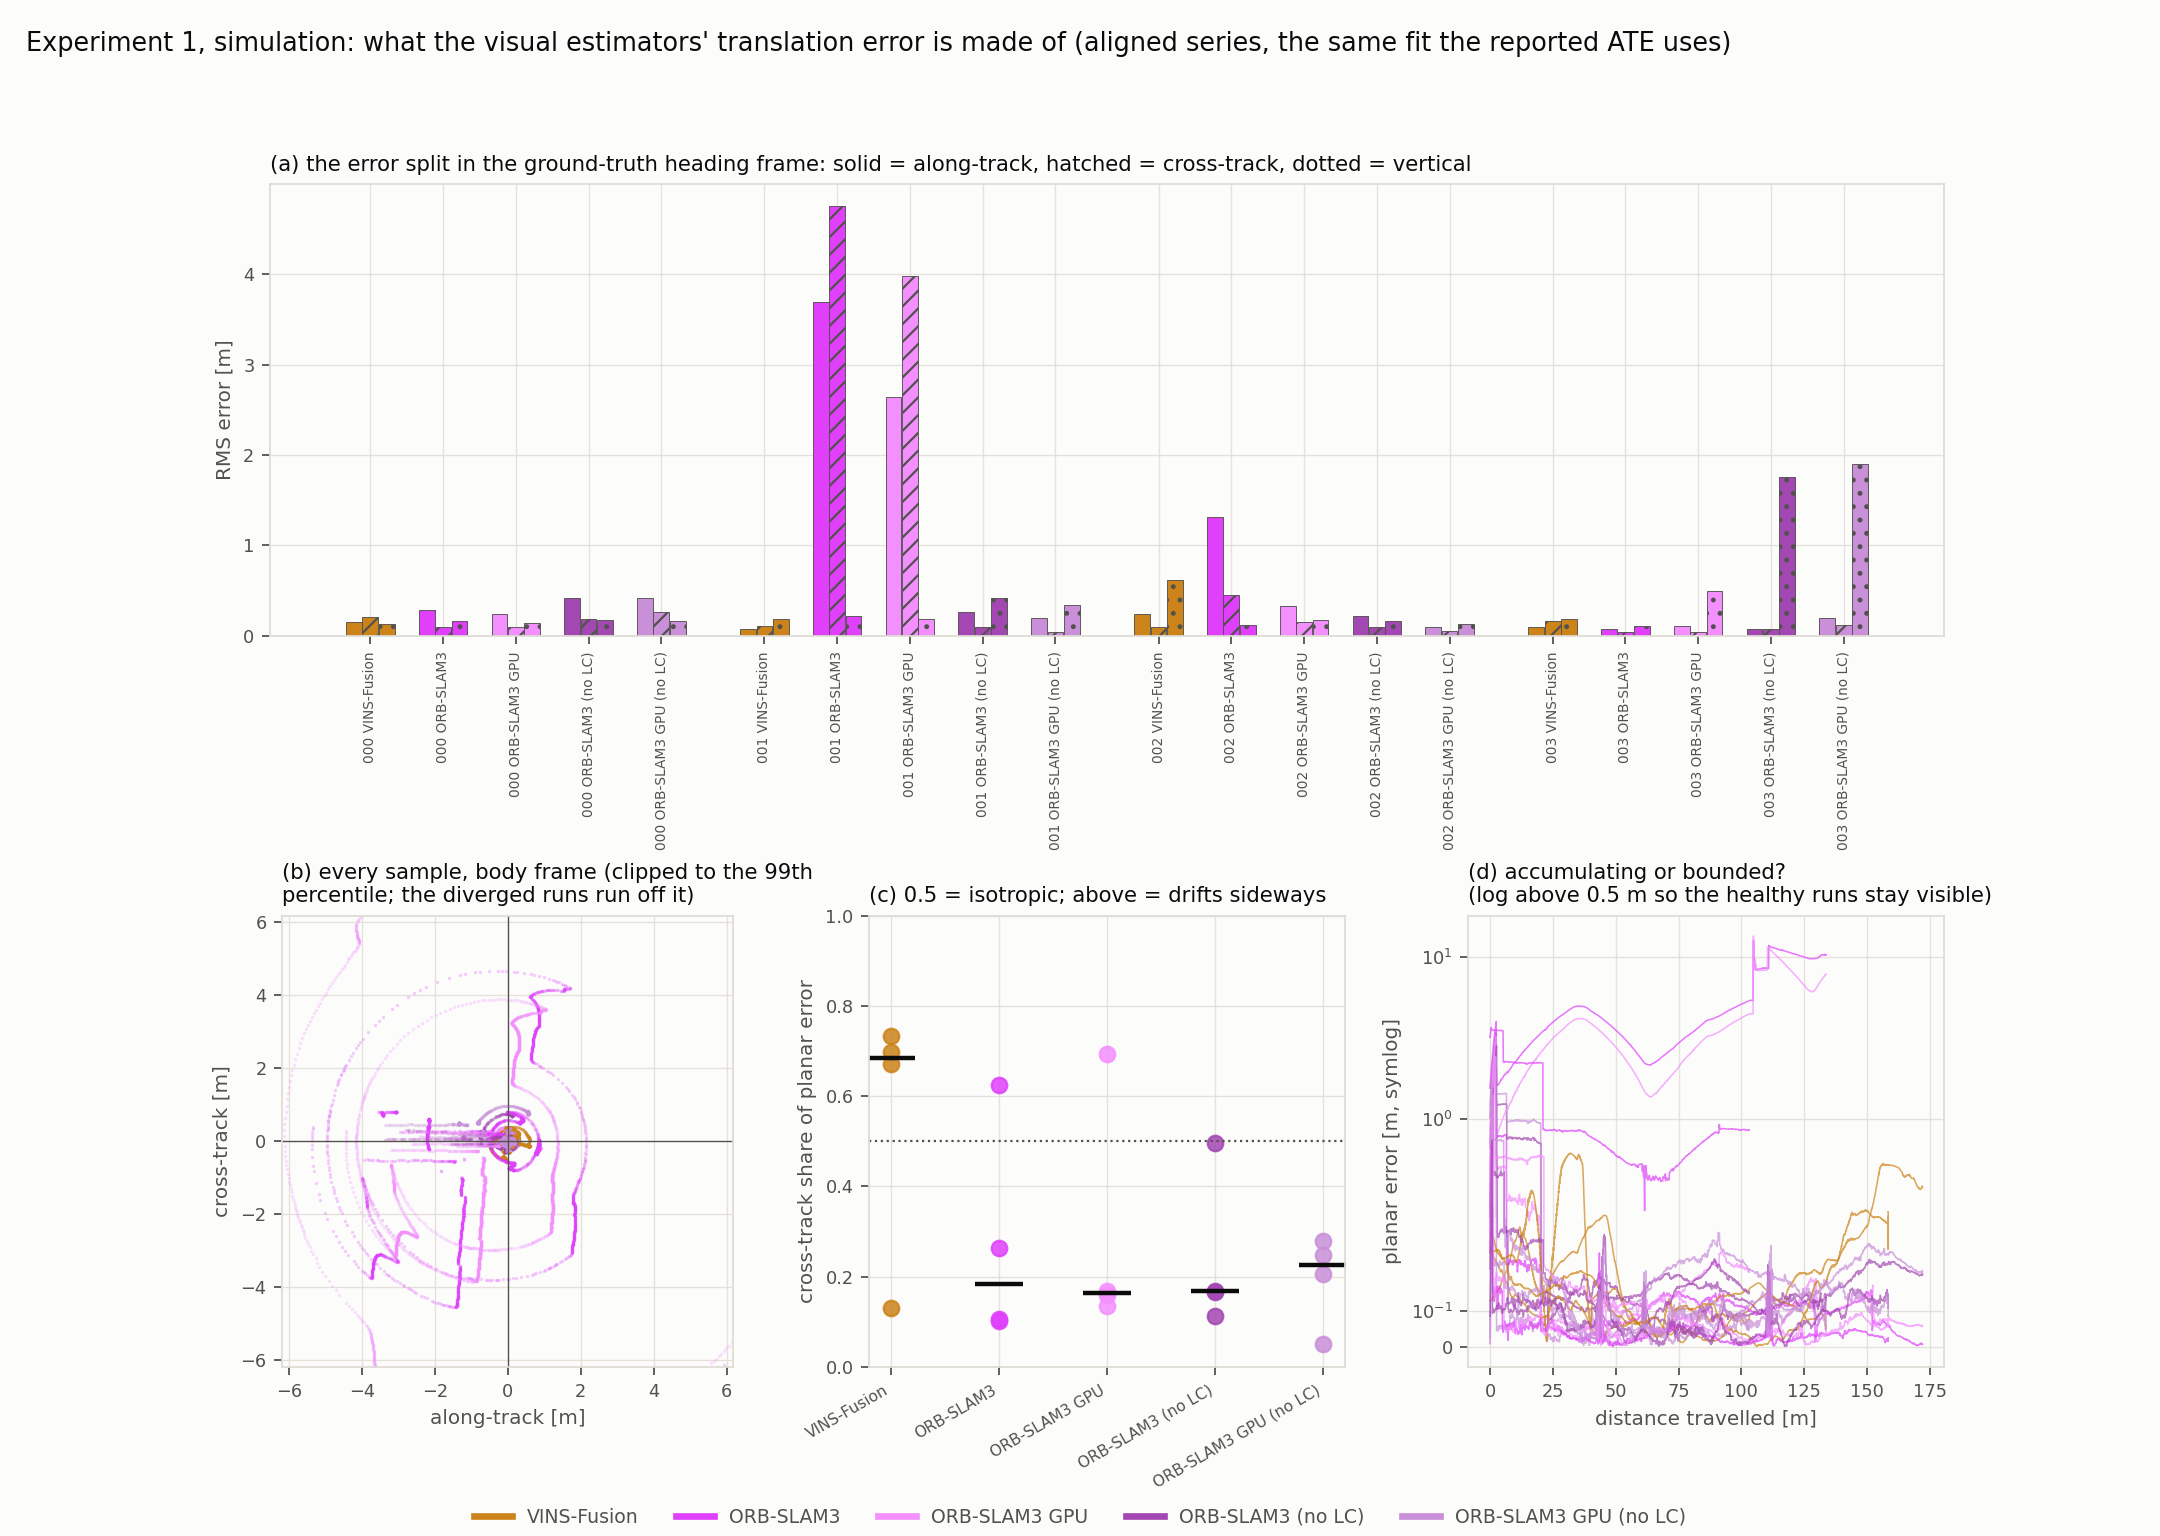
\includegraphics[width=\textwidth]{figures/exp1_translation_pattern.png}
  \caption[What the visual estimators' translation error is made of.]{What the
  translation error is made of, on the aligned series the reported ATE uses.
  (a) the error split per run into along-track, cross-track and vertical;
  (b) every sample in the body frame, clipped to the 99th percentile because
  the five diverged runs reach metres; (c) the cross-track share of the planar
  error, where \num{0.5} is isotropic and above it the estimate drifts
  sideways; (d) error against distance travelled, on a symmetric-log axis above
  \SI{0.5}{\metre} so that the eighteen runs that held tracking stay visible.}
  \label{fig:exp1-translation-pattern}
\end{figure}

\begin{figure}[p]
  \centering
  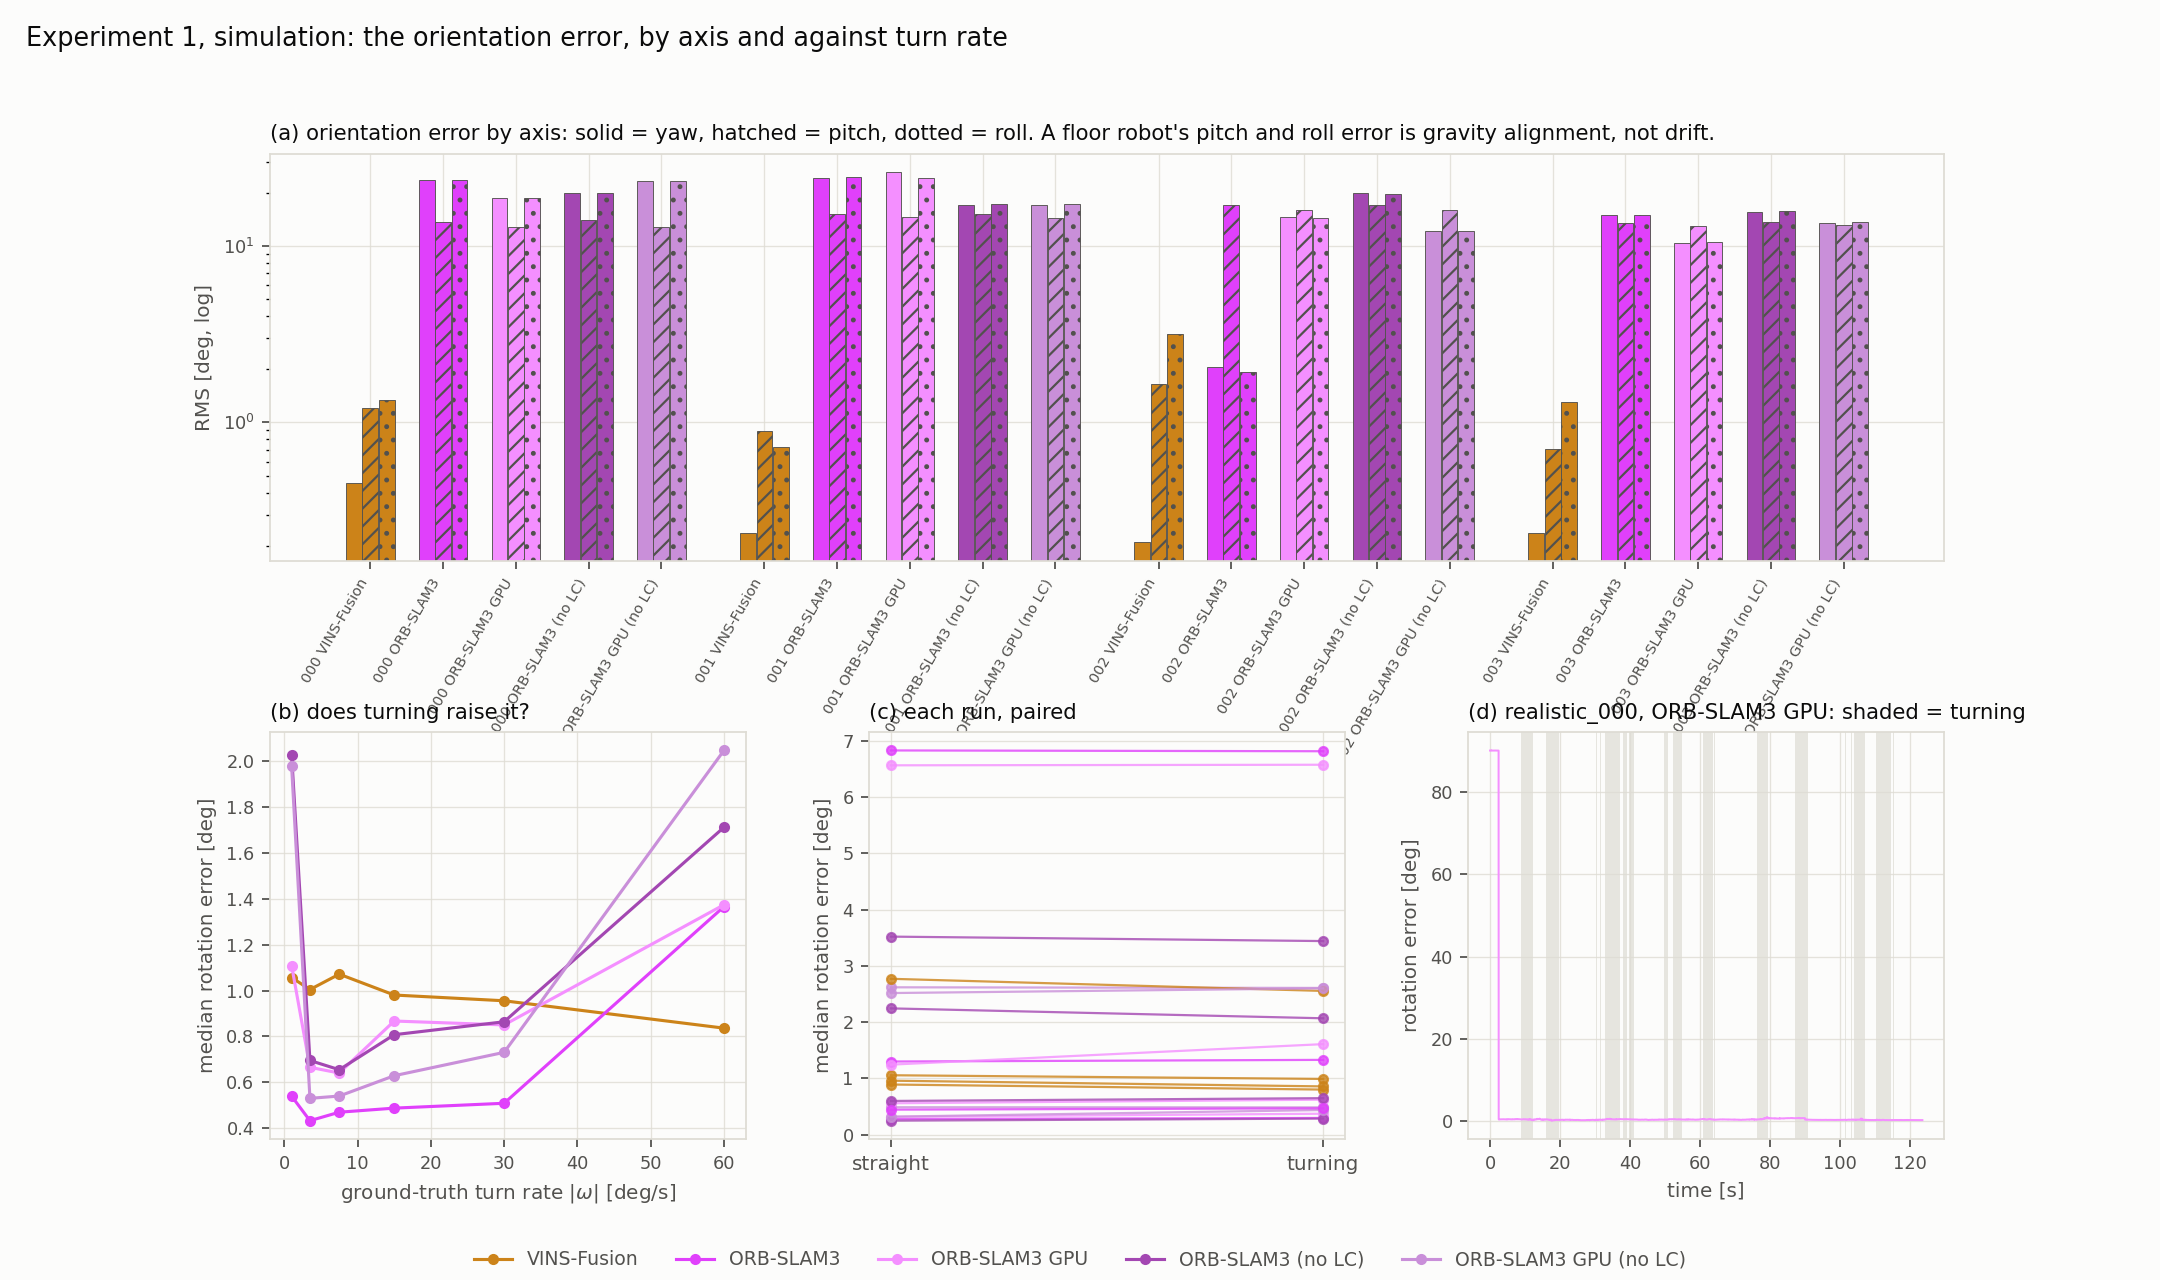
\includegraphics[width=\textwidth]{figures/exp1_rotation_pattern.png}
  \caption[The orientation error by axis and against turn rate.]{The
  orientation error. (a) yaw, pitch and roll RMS per run on a logarithmic axis;
  (b) median rotation error binned by the ground truth's own turn rate;
  (c) the same two medians paired within each run; (d) one run's rotation error
  against time, with the turning segments shaded.}
  \label{fig:exp1-rotation-pattern}
\end{figure}

\paragraph{Latency and resources.} By the design decision of 6 November
2026 the real-time and resource measurement of this experiment is taken only
on the two mapping recordings, each configuration run three times:
\repo{dataset_allsensor_realistic_map} (U layout, \SI{286}{\second}, 8\,725
stereo pairs) and \repo{dataset_allsensor_realistic_01_map} (I layout,
\SI{315}{\second}, 9\,552 pairs). Eighteen runs exist, six configurations of
three repeats each at replay rate 1.0 with no detector: ORB-SLAM3 with the
CPU and with the GPU front end, loop closer disabled, and VINS-Fusion
(\cref{tab:mapping-resources}). The repeats are tight, front-end medians
within \SIrange{1}{7}{\milli\second} of their mean and peak memory within
\SI{30}{\mebi\byte}.

The two pipelines divide the cost differently, and neither is cheaper than
the other outright. VINS-Fusion optimises in \SI{44}{\milli\second} where
ORB-SLAM3's local mapping takes \SIrange{211}{406}{\milli\second}, and holds
its state in a quarter of the memory, but spends more than twice the
processor time: about eight cores of one against three and a half. Their
front ends are within \SI{6}{\milli\second} of each other, and every
configuration keeps \SIrange{75}{96}{\percent} of the bag's frames, so the
choice between them is a memory-against-cores trade, not a speed one.

Between ORB-SLAM3's two front ends the recordings disagree. On the U
recording the GPU extractor behaves as the single runs showed, tracking in
\SI{37}{} against \SI{42}{\milli\second} and keeping \SI{96}{} against
\SI{93}{\percent} of frames; on the I recording the sign reverses, \SI{52}{}
against \SI{44}{\milli\second} and \SI{75}{} against \SI{91}{\percent} kept,
with the local-mapping median at \SI{406}{\milli\second}. VINS-Fusion reads
the same on both recordings (front end \SI{38.1}{} and \SI{38.6}{},
back end \SI{44.3}{} and \SI{44.5}{\milli\second}), so the recordings
themselves do not impose a difference of that size.

\begin{queried}[Confound: run order] The six GPU runs were made consecutively
from 21:04 to 22:04 and the six CPU runs from 23:27 to 00:18, so the
I-recording GPU repeats were the fourth to sixth GPU runs of a session on a
laptop that throttles at \SI{90}{\celsius}; the front-end record notes that
timing comparisons need a cool-start, interleaved order. The six VINS-Fusion
runs are a separate session of 7 November and are not a control for that
state. The U-recording figures are the ones to quote until the I recording is
repeated interleaved. \end{queried} 
\reporttable{mapping_resources}

\paragraph{What each accuracy run cost.} The twenty accuracy runs were
measured for cost as well, on the same machine and in the same sessions, and
\cref{tab:realistic-resources} reports them one row per run. They are not a
substitute for \cref{tab:mapping-resources}: they are single runs on four
short recordings rather than three repeats on two long ones, and the
divergences of \cref{tab:realistic-baseline} are inside them. What they add is
that accuracy and cost can be read on the same runs, which
\cref{fig:realistic-cost-accuracy} draws.

The separation between the two pipelines is the one the mapping recordings
show, at the same sizes. VINS-Fusion holds its state in \SIrange{477}{492}{\mebi\byte}
against ORB-SLAM3's \SIrange{1029}{1350}{\mebi\byte} and optimises in
\SIrange{45}{60}{\milli\second} against \SIrange{189}{286}{\milli\second},
for \SIrange{707}{801}{\percent} of one core against
\SIrange{285}{448}{\percent}. Within ORB-SLAM3 the GPU front end tracks in
\SIrange{29.6}{36.7}{\milli\second} against the CPU front end's
\SIrange{49.2}{54.9}{\milli\second} and draws about a core less, at
\SI{150}{\mebi\byte} more memory. These runs were not interleaved either, so
they carry the same thermal caveat as \cref{tab:mapping-resources} and are
quoted as a second observation of the same separation, not as an independent
one.

The figure's own result is a negative one: no panel shows cost buying
accuracy. Every run that diverged is ORB-SLAM3, and within each front end the
diverged runs cost what the runs that held cost --- with the GPU front end
\SIrange{31.6}{36.7}{\milli\second} against \SIrange{29.6}{36.2}{\milli\second},
overlapping entirely, and with the CPU front end
\SIrange{52.6}{54.9}{\milli\second} against \SIrange{49.2}{51.6}{\milli\second},
a gap of one to five milliseconds across three runs and two recordings, which
one run per cell cannot separate from the recording. A run about to be thrown
several metres by a false loop closure is not working harder beforehand, so no
resource measure on this machine is a usable early warning for the failure
mode this experiment actually found.

\reporttable{realistic_resources}

\begin{figure}[htbp]
  \centering
  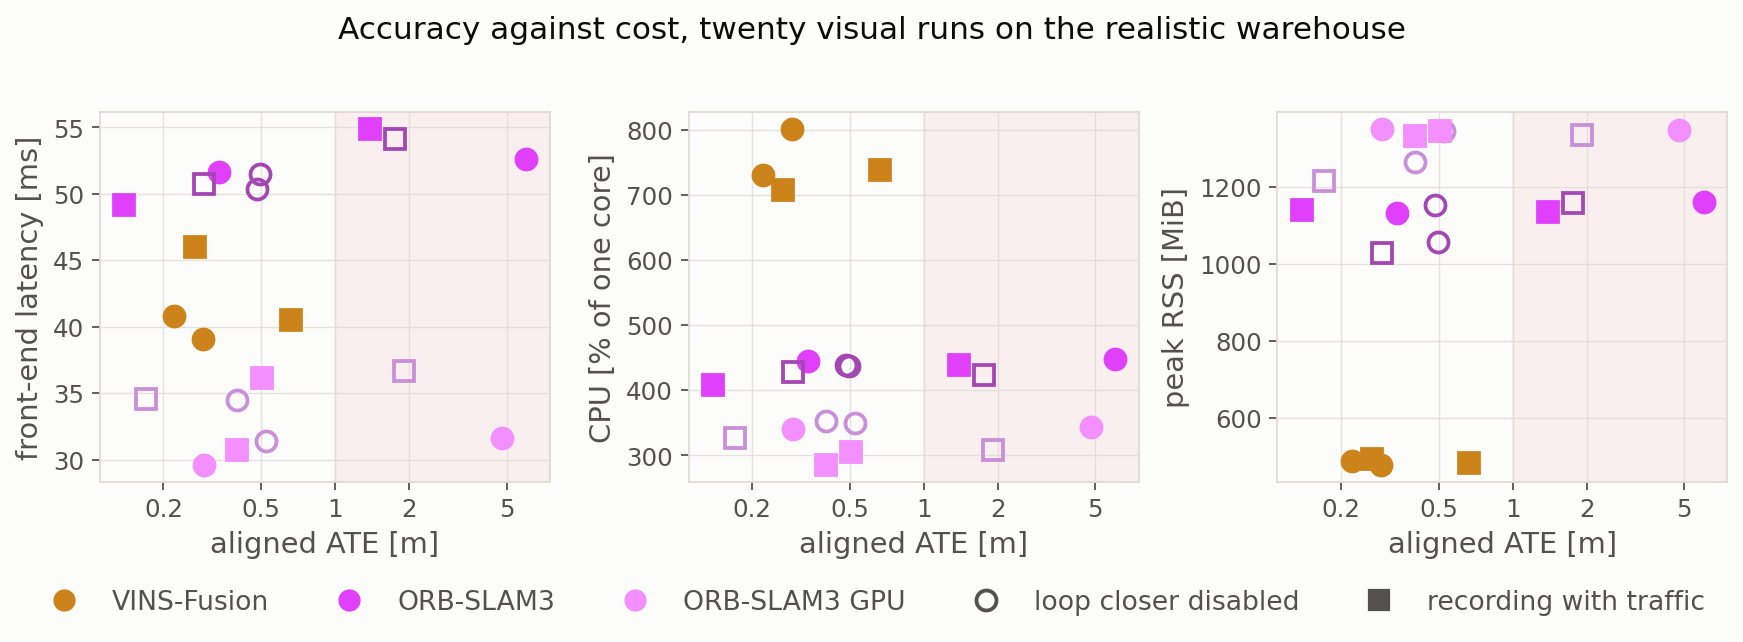
\includegraphics[width=\textwidth]{figures/realistic_cost_accuracy.png}
  \caption[Accuracy against cost on the twenty realistic-world runs.]{Accuracy
  against cost, one point per visual run on the four realistic-warehouse
  recordings, from \cref{tab:realistic-baseline,tab:realistic-resources}.
  Aligned ATE is on a logarithmic axis in all three panels; the shaded band is
  the region above \SI{1}{\metre}, which holds the five diverged runs. Orange
  is VINS-Fusion, magenta ORB-SLAM3 with the CPU front end and light magenta
  with the GPU front end; an open marker is a run with the loop closer
  disabled and a square a recording carrying traffic. Cost is the run's median
  front-end latency, its process time as a percentage of one core, and its
  peak resident set.}
  \label{fig:realistic-cost-accuracy}
\end{figure}



\paragraph{How repeatable is any of this?} The eighteen runs above are the only
repeated runs in the simulation campaign, and scoring them for accuracy as well
as for time measures something no other result in this chapter can:
how much an estimate moves when nothing changes.
\Cref{tab:mapping-repeats} gives the spread over the three repeats of each
configuration. The two estimators answer differently. VINS-Fusion repeats to
\SI{0.094}{\metre} on the U recording and \SI{0.035}{} on the I, five and
seven per cent of its own mean. ORB-SLAM3 does not: its three repeats span
\SI{0.089}{\metre} on the U recording and \SI{0.277}{} on the I with the CPU
front end, and \SI{0.016}{} and \SI{0.236}{\metre} with the GPU front end ---
on the I recording that is half to four fifths of the configuration's own mean,
from the same binary, the same configuration file and the same bag, with the
loop closer disabled in all six.

The frame counts in the same table are consistent with why. VINS-Fusion
processed every frame of both recordings in all six runs, so it saw identical
input each time; ORB-SLAM3 kept \SIrange{90}{97}{\percent} with the CPU front
end and \SIrange{70}{98}{\percent} with the GPU one, and which frames a run
loses depends on how the laptop was scheduling at that moment. That is a
consistent explanation and not a demonstrated one: a keyframe-based system with
a bundle adjustment on its own thread need not be deterministic even on
identical input. Separating the two would need a run at a replay rate slow
enough to drop nothing, which this chapter does not have. The worst spread also
belongs to the I recording, whose repeats carry the thermal confound noted
above, so part of \SI{0.277}{\metre} may be the laptop rather than the
estimator.

Read against \cref{tab:realistic-baseline} this sets a floor under what that
table can be asked. A difference of less than about a quarter of a metre
between two ORB-SLAM3 arms is inside the spread measured here and should not be
read as an effect; this is the quantity the bold marking of that table was
hedged against, now measured. Two of the chapter's findings survive it and one
is strengthened. The five divergences are \SIrange{1.39}{6.02}{\metre}, five to
twenty times the floor, and the false closure that causes the largest of them
is reproduced by both front ends on the same frame. The claim that the front
end changes throughput and not accuracy is supported rather than weakened:
the CPU and GPU arms differ by less than this floor on every recording, which
is what having no effect looks like. What should not be carried further is any
ordering of two ORB-SLAM3 arms that rests on a gap smaller than it.

\reporttable{mapping_repeats}

\paragraph{Limitations, each stated once.} \emph{$n$:} one run per cell on the
four accuracy recordings, in both families; the three repeats of each
mapping-recording configuration (\cref{tab:mapping-repeats}) are the only
within-configuration spread the campaign measures, and they are on different
routes. \emph{Equal handicap, not equal effort:} the shared inertial model
was fitted to neither family. \emph{Idealised wheels:} simulated encoders
with slip under \SI{1}{\percent}, the proprioceptive estimators' best case.
\emph{Route and traffic confounded:} no two recordings share a route, so
traffic is a condition of a recording and not a tested factor.
\emph{Three-dimensional ATE:} the metric charges vertical drift to a floor
robot; the planar onset table is the complement, not a replacement.
\emph{Deployment rate on one laptop:} frame retention and every latency
figure are properties of this machine at rate 1.0, and the mapping-bag
repeats were not interleaved between front ends. \emph{Run bookkeeping:} one
directory held a run on another recording for a day; the manifest caught it,
and the launch should refuse an output directory whose name disagrees with
its dataset.

\begin{queried}[Resolved: \repo{realistic_002/loopclosing_gpu}]
Earlier on 6 November this run was reported as closure-free from its
\repo{loop_closing.csv} and queried. Its manifest shows the real cause: it was
launched on the \repo{realistic_003} bag with \repo{realistic_002}'s output
path, so it was scored against the wrong truth (\SI{4.94}{\metre},
\SI{48.9}{\degree}, 139\,\% of the recording's frames processed). It is set
aside, not deleted; the configuration was re-run on the right bag the same
evening and every table here carries that run.
\end{queried}

\begin{queried}[Open: the false closure is diagnosed from its correction, not from the images]
The \SI{14}{\metre} correction and the one-aisle keyframe separation identify
the \repo{realistic_001} closure as false, and both front ends agree; the
matched image pair has not been inspected, and the two April-style guards
that would catch it (a covisibility-consistency window, or a maximum
correction against the inertial drift bound) are untested. Until one is, the
finding is a diagnosis, not a fix.
\end{queried}

\paragraph{Summary.} Two families were scored on the same four recordings.
Among the non-visual estimators IMU-only dead reckoning drifts by
\SIrange{12}{23}{\metre} and wheel odometry by \SIrange{1.0}{4.8}{\metre} of
aligned ATE; the EKF, run on the visual systems' own inertial noise as the
design requires, holds \SIrange{0.68}{2.80}{\metre}, while the same filter on
a measured noise model would hold \SIrange{0.21}{0.58}{\metre}. Among the
visual ones VINS-Fusion holds \SIrange{0.22}{0.66}{\metre} with no jump and
is worst on the U layout with traffic; ORB-SLAM3 holds
\SIrange{0.14}{0.52}{\metre} in eleven runs of sixteen, and its five
divergences are the loop closer's: a false closure on the I layout's repeated
aisles that puts both front ends \SIrange{4.8}{6.0}{\metre} off, a vertical
drift on the same layout with traffic that only the closer corrects, and one
initialisation offset. Neither pipeline loses tracking on any recording, with
or without traffic, and the front end changes throughput
(\SIrange{97}{99}{\percent} of frames kept against \SIrange{72}{94}{\percent})
and not accuracy. Across the families the EKF at the shared handicap loses to
VINS-Fusion on every recording and the measured-noise diagnostic beats it on
three of four, so on these routes the noise model is worth more than the
choice of estimator. Against the project's target of \SI{0.05}{\metre} ATE no
estimator qualifies; against the \SI{1.5}{\metre} RPE bound at
\SI{1}{\second}, all but the IMU do. On cost, VINS-Fusion optimises five to
nine times faster than ORB-SLAM3's local mapping and in a quarter of the
memory, for more than twice the processor time.

\paragraph{Future plan.} Fit the visual systems' inertial noise to this
platform rather than copying a file, since the slot shows the noise model is
worth more than the estimator; feed the VIO pose into the EKF as a third
measurement; add a correction bound to the loop closer and test it on
\repo{realistic_001}; repeat the mapping-recording runs interleaved between
all three configurations from a cool start, so that the thermal state is
shared rather than confounded with the configuration; and record a second
route in each layout so that traffic and route are separable.

% =====================================================================
\FloatBarrier

\section{Real robot}
\label{sec:exp1-real}

\slotstatus{partial}{Four real recordings with an independent planar reference
(\repo{dataset_realv6_000}, \repo{dataset_realv7_000} to \repo{_002}). A
non-visual baseline exists: wheel+gyro dead reckoning with the feedback speed
scaled by a factor fitted once against the tracker on \repo{realv7_000} and
held on the other three. The visual arm is ORB-SLAM3 in four configurations on
each recording, sixteen runs, all made with the fork's patch-15
initialisation switches and scored with no repair applied; they give
\SIrange{0.404}{0.480}{\metre} on \repo{realv6_000},
\SIrange{0.251}{0.268}{} on \repo{realv7_000}, \SIrange{0.442}{1.278}{} on
\repo{_001} and \SIrange{0.172}{0.198}{} on \repo{_002}. Across the held
recordings the two families are in the same accuracy class, the baseline
leading on one, tying on one and losing the third. The EKF of the simulation
slot cannot be formed, because the rig publishes no steering measurement;
VINS-Fusion has no valid run on any recording; and every value is provisional
until the marker-to-IMU lever arm is measured.}

\paragraph{Objective.} The real-robot half of the simulation question: do the
visual pipelines track the robot against an independent reference, and does a
non-visual estimator match them on the same recordings.

\paragraph{Process.} Two groups of runs share these recordings.


\emph{Non-visual.} The bags carry \repo{/feedback/velocity} and
\repo{/feedback/steering} (\SI{50}{\hertz}, \texttt{std\_msgs/Float64}) and
the WitMotion yaw sensor on \repo{/hwt101ct_yaw_publisher} (\SI{200}{\hertz}).
The velocity is in a firmware unit, not metres per second; the steering is a
command echo that takes two values (0 and $-30$) on every recording and so
carries no yaw rate; the yaw sensor's orientation field is identity and its
rate on the $y$ axis is the live gyro (the sensor is mounted with $y$
vertical: that axis integrates to \SI{6.29}{rad} over \repo{realv7_000}, whose
tracker heading sweeps \SI{6.3}{rad}; $x$ and $z$ integrate to under
\SI{0.05}{rad}).

\repo{script/real_wheel_baseline.py} integrates heading from
that gyro with its rest bias removed (\SIrange{3}{7}{\second} at rest at the
head of each bag) and position from the scaled speed. The scale $k$, the gyro
axis and its sign are fitted on \repo{realv7_000} alone by minimising the
planar ATE after rigid $SE(2)$ alignment with scale fixed (a wrong sign
mirrors the path, which a proper rotation cannot align), then held: the fit
recording's own score is a calibration, the three held scores are the result.
The fitted $k=0.325$ agrees with the plain path-length ratio of each
\repo{realv7} bag (0.323 to 0.329). The time offset between tracker and bag is
the wheel-speed cross-correlation of \repo{script/eval_real_gt.py}
($r=0.93$ to $0.99$ on \repo{realv7}, $0.61$ on the sparse \repo{realv6}
export), scoring is that script's planar procedure at the tracker's own
samples, and the one off-path \repo{realv6} sample is removed by the rule the
realv6 analysis fixed.

The rig's wheelbase, \SI{0.60}{\metre}, is recorded
and unused: with no steering measurement there is nothing to put through a
bicycle model, so the yaw-rate observation that gives the simulation EKF its
bias state does not exist, and that filter would reduce to this integration.


\emph{Visual.} The bag was replayed into each node at real time on the
afternoon of 3 November 2026; no detector ran. ORB-SLAM3 used
\repo{config/wil/stereo_imu.yaml} with the repaired library (fork patches
11--14b, node and library built alike), the 3 November stereo extrinsic and
\texttt{IMU.NoiseGyro} 0.1 with \texttt{IMU.NoiseAcc} 1.0, ten times the values
that had been copied from the VINS file, in four configurations: GPU or CPU
feature extractor, loop closing on or off. VINS-Fusion used the same file with
the gravity norm of an August recording. Earlier runs on this bag were
overwritten by these and are not reported. The optical tracker export was scored
with the real-robot procedure of Experiment~1.

\paragraph{Dataset.} \SI{220}{\second}, 6\,601 stereo pairs at \SI{30}{\hertz},
RealSense IMU at \SI{200}{\hertz} on the inherited topic name, wheel-speed
feedback, a figure-of-eight of about \SI{27}{\metre} at a median
\SI{0.15}{\metre\per\second} on the Gensurv floor, no scripted moving objects.
Tracker export: 277 samples, median spacing \SI{0.6}{\second}, 66 gaps above
\SI{1}{\second}, one sample \SI{5.2}{\metre} off the path at \SI{184.9}{\second}.

\paragraph{Datasets.} The four real recordings that carry an independent
planar reference: routes of \SIrange{22}{37}{\metre} over
\SIrange{97}{219}{\second}. Sources:
\path{output/compare/real/exp1-wheel/} (\repo{wheel_metrics.csv},
\repo{manifest.json}), estimates under \path{output/output_wheel/real/}.

\paragraph{Reporting rules, visual arms.} \path{script/eval_real_gt.py}: rigid SE(2)
alignment with scale fixed, lever arm set to zero and unmeasured, every value
provisional. The export fails the tool's gap and step rules, so the tool labels
each run \emph{failed (ground truth invalid)}; the values below are diagnostics.
All are scored with the one off-path sample removed, an edit recorded here and
applied nowhere else; \cref{tab:realv6-cleaning} shows what that sample does to
one run. The bag was not on the machine, so the time offset is pinned to the
value the wheel-speed cross-correlation found on 2 November and the manifests
record the substitution. Sources: \path{output/compare/real/realv6_1103pm_*/},
\path{output/compare/real/realv6-insights/}, run directories under
\path{output/output_orb/real/dataset_realv6_000/} and
\path{output/output_vins/real/dataset_realv6_000/}.

\subsubsection{Non-visual baseline}

\paragraph{Results.} \Cref{tab:exp1-real-wheel} and \cref{fig:exp1-real-wheel}.
On the fit recording the baseline reads \SI{0.06}{\metre} ATE with a path ratio
of 0.99, which is the calibration. Held, it reads \SI{0.26}{} and
\SI{0.22}{\metre} on \repo{realv7_001} and \repo{_002} with path ratios of
0.99 and 1.01, and \SI{0.46}{\metre} on \repo{realv6_000} against its sparse
export, with no jump and a relative error at \SI{1}{\second} of
\SIrange{0.01}{0.02}{\metre}.

% Generated by script/real_wheel_baseline.py -- do not edit by hand.
\begin{table}[htbp]
\centering
\caption[Wheel+gyro dead reckoning against the optical tracker.]{Wheel+gyro dead reckoning on the real recordings against the optical tracker: the feedback speed scaled by $k$ (fitted on \repo{realv7_000} by minimising planar ATE, held on the others), heading from the integrated gyro with its rest bias removed, rigid $SE(2)$ alignment with scale fixed, lever arm zero and unmeasured. ATE at the tracker's samples; path ratio is estimated over true path length.}
\label{tab:exp1-real-wheel}
\small
\resizebox{\textwidth}{!}{%
\begin{tabular}{llrrrrrrr}
\toprule
Recording & Role & $k$ & Offset [\si{\second}] ($r$) & Samples & ATE RMSE [\si{\metre}] & ATE max [\si{\metre}] & Path ratio & RPE$_{1\,\mathrm{s}}$ [\si{\metre}] \\
\midrule
\repo{realv7_000} & fit & 0.325 & -2.57 (0.99) & 491 & 0.057 & 0.11 & 0.990 & 0.008 \\
\repo{realv7_001} & held & 0.325 & -3.77 (0.98) & 632 & 0.259 & 0.47 & 0.988 & 0.021 \\
\repo{realv7_002} & held & 0.325 & -2.60 (0.93) & 499 & 0.219 & 0.27 & 1.006 & 0.008 \\
\repo{realv6_000} & held & 0.325 & -4.14 (0.61) & 233 & 0.463 & 0.70 & 1.041 & 0.015 \\
\bottomrule
\end{tabular}}
\end{table}


\begin{figure}[htbp]
  \centering
  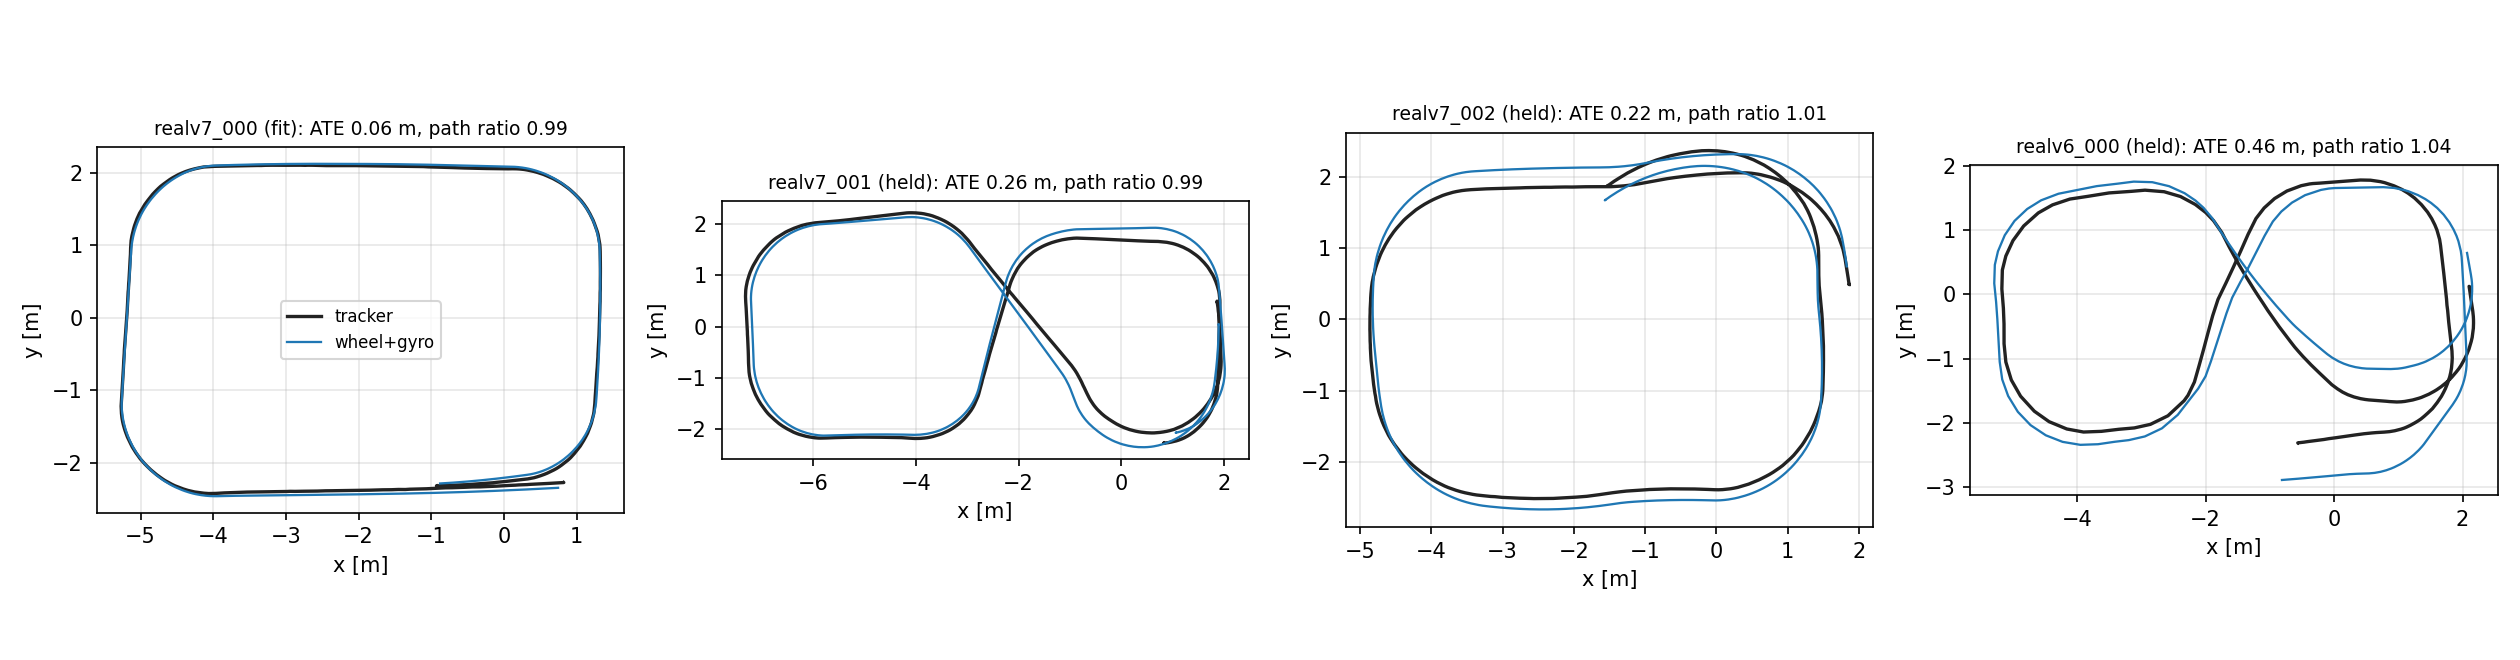
\includegraphics[width=\textwidth]{../../../../output/compare/real/exp1-wheel/wheel_paths_light.png}
  \caption[Wheel+gyro dead reckoning against the tracker.]{Wheel+gyro dead
  reckoning (blue) against the tracker (black) after
  rigid planar alignment, one panel per recording; the first is the recording
  the speed scale was fitted on.}
  \label{fig:exp1-real-wheel}
\end{figure}

\paragraph{Analysis.} The comparison this slot exists for now has a number on
both sides, and it does not favour vision. On the same recordings the best
ORB-SLAM3 configuration reads \SI{0.44}{\metre} on \repo{realv7_001},
\SI{0.47}{\metre} on \repo{realv7_002} and \SI{0.46}{\metre} on
\repo{realv6_000} (the real-robot section below, after the scorer's frame
repair); the scaled dead reckoning reads \SI{0.26}{}, \SI{0.22}{} and
\SI{0.46}{\metre}, with path ratios within \SI{4}{\percent} of one where the
visual runs read \SIrange{5}{15}{\percent} long.

Three things bound that reading. The scale is a fitted constant, not a measured one, so the baseline
has had one parameter tuned against the truth it is scored on, on a different
recording; a second calibration route, the wheel circumference and the gear
ratio, would remove that. The routes are \SIrange{22}{37}{\metre} with the
robot at \SI{0.2}{\metre\per\second}: a gyro drifting at the measured rest
bias of \SIrange{0.003}{0.006}{\radian\per\second} accumulates
\SIrange{0.3}{1.3}{\radian} over a run if the bias is not removed and under
\SI{0.1}{\radian} after the rest-window removal, and on a longer route that
term grows while the visual error need not. And the lever arm is zero for
both sides. Against the project's targets no run approaches \SI{0.05}{\metre}
except the calibration itself; every run is inside the \SI{1.5}{\metre} RPE
bound.

\begin{queried}[Open: the realv6 scale]
On \repo{realv6_000} the path-length ratio gives $k=0.43$ where the three
\repo{realv7} bags give $0.32$ to $0.33$, yet the held $k=0.325$ scores a path
ratio of 1.04 on the matched samples. The export is at \SI{1.7}{\hertz} and
fails the validity rules, and the recording predates \repo{realv7} by three
days; whether the firmware unit changed or the sparse export misstates the
path length is not decided, and the \repo{realv6} row is a diagnostic.
\end{queried}

\subsubsection{Visual estimators}

\paragraph{Results.} ORB-SLAM3 follows the whole \SI{218}{\second} route in
every configuration: \SI{0.52}{} and \SI{0.46}{\metre} with the GPU extractor
(loop closing on and off), \SI{0.62}{} and \SI{1.03}{\metre} with the CPU
extractor, which drops two thirds of the frames at real time
(\cref{tab:realv6-final}, \cref{fig:realv6-paths}). VINS-Fusion tracked
\SI{18}{\second} before 217 IMU-gap resets took over (\cref{tab:realv6-vins})
and has no entry in the accuracy table.

\begin{table}[htbp]
\centering
\scriptsize\setlength{\tabcolsep}{3pt}
\caption[Realv6: every surviving run against the cleaned tracker truth.]{ORB-SLAM3 on \repo{dataset_realv6_000} against the cleaned tracker truth, 3 November 2026 afternoon series: repaired library, replay rate 1.0, 3 November stereo extrinsic, \texttt{IMU.NoiseGyro} 0.1 and \texttt{IMU.NoiseAcc} 1.0, GPU or CPU feature extractor, loop closing (LC) on or off. Aligned planar ATE after a rigid SE(2) fit with scale fixed; RPE at \SI{1}{\second} translational; path ratio = estimate / truth; resets = \repo{local_mapping_bad_imu} map resets; dropped = camera frames the node's queue discarded of about 6\,480 received. Lever arm tracker-marker to IMU unmeasured (zero applied); time offset pinned to \SI{-4.14}{\second}; all values provisional under the scorer's validity rules. \\textbf{Bold} marks the lowest ATE of the five runs; with one run per configuration that records which run came lowest, not that the configuration is better.}
\label{tab:realv6-final}
\begin{tabular}{lrrrrrrr}
\toprule
Run & ATE [m] & median [m] & max [m] & RPE$_{1\,\mathrm{s}}$ [m] & path ratio & resets & dropped \\
\midrule
ORB-SLAM3, GPU, LC on & 0.52 & 0.44 & 1.11 & 0.057 & 0.85 & 2 & 2420 \\
ORB-SLAM3, CPU, LC on & 0.62 & 0.48 & 1.38 & 0.110 & 0.88 & 2 & 4363 \\
ORB-SLAM3, GPU, LC off & \textbf{0.46} & 0.36 & 0.99 & 0.056 & 0.87 & 0 & 3201 \\
ORB-SLAM3, CPU, LC off & 1.03 & 0.89 & 1.83 & 0.223 & 0.96 & 3 & 4204 \\
\bottomrule
\end{tabular}
\end{table}


\begin{figure}[p]
  \centering
  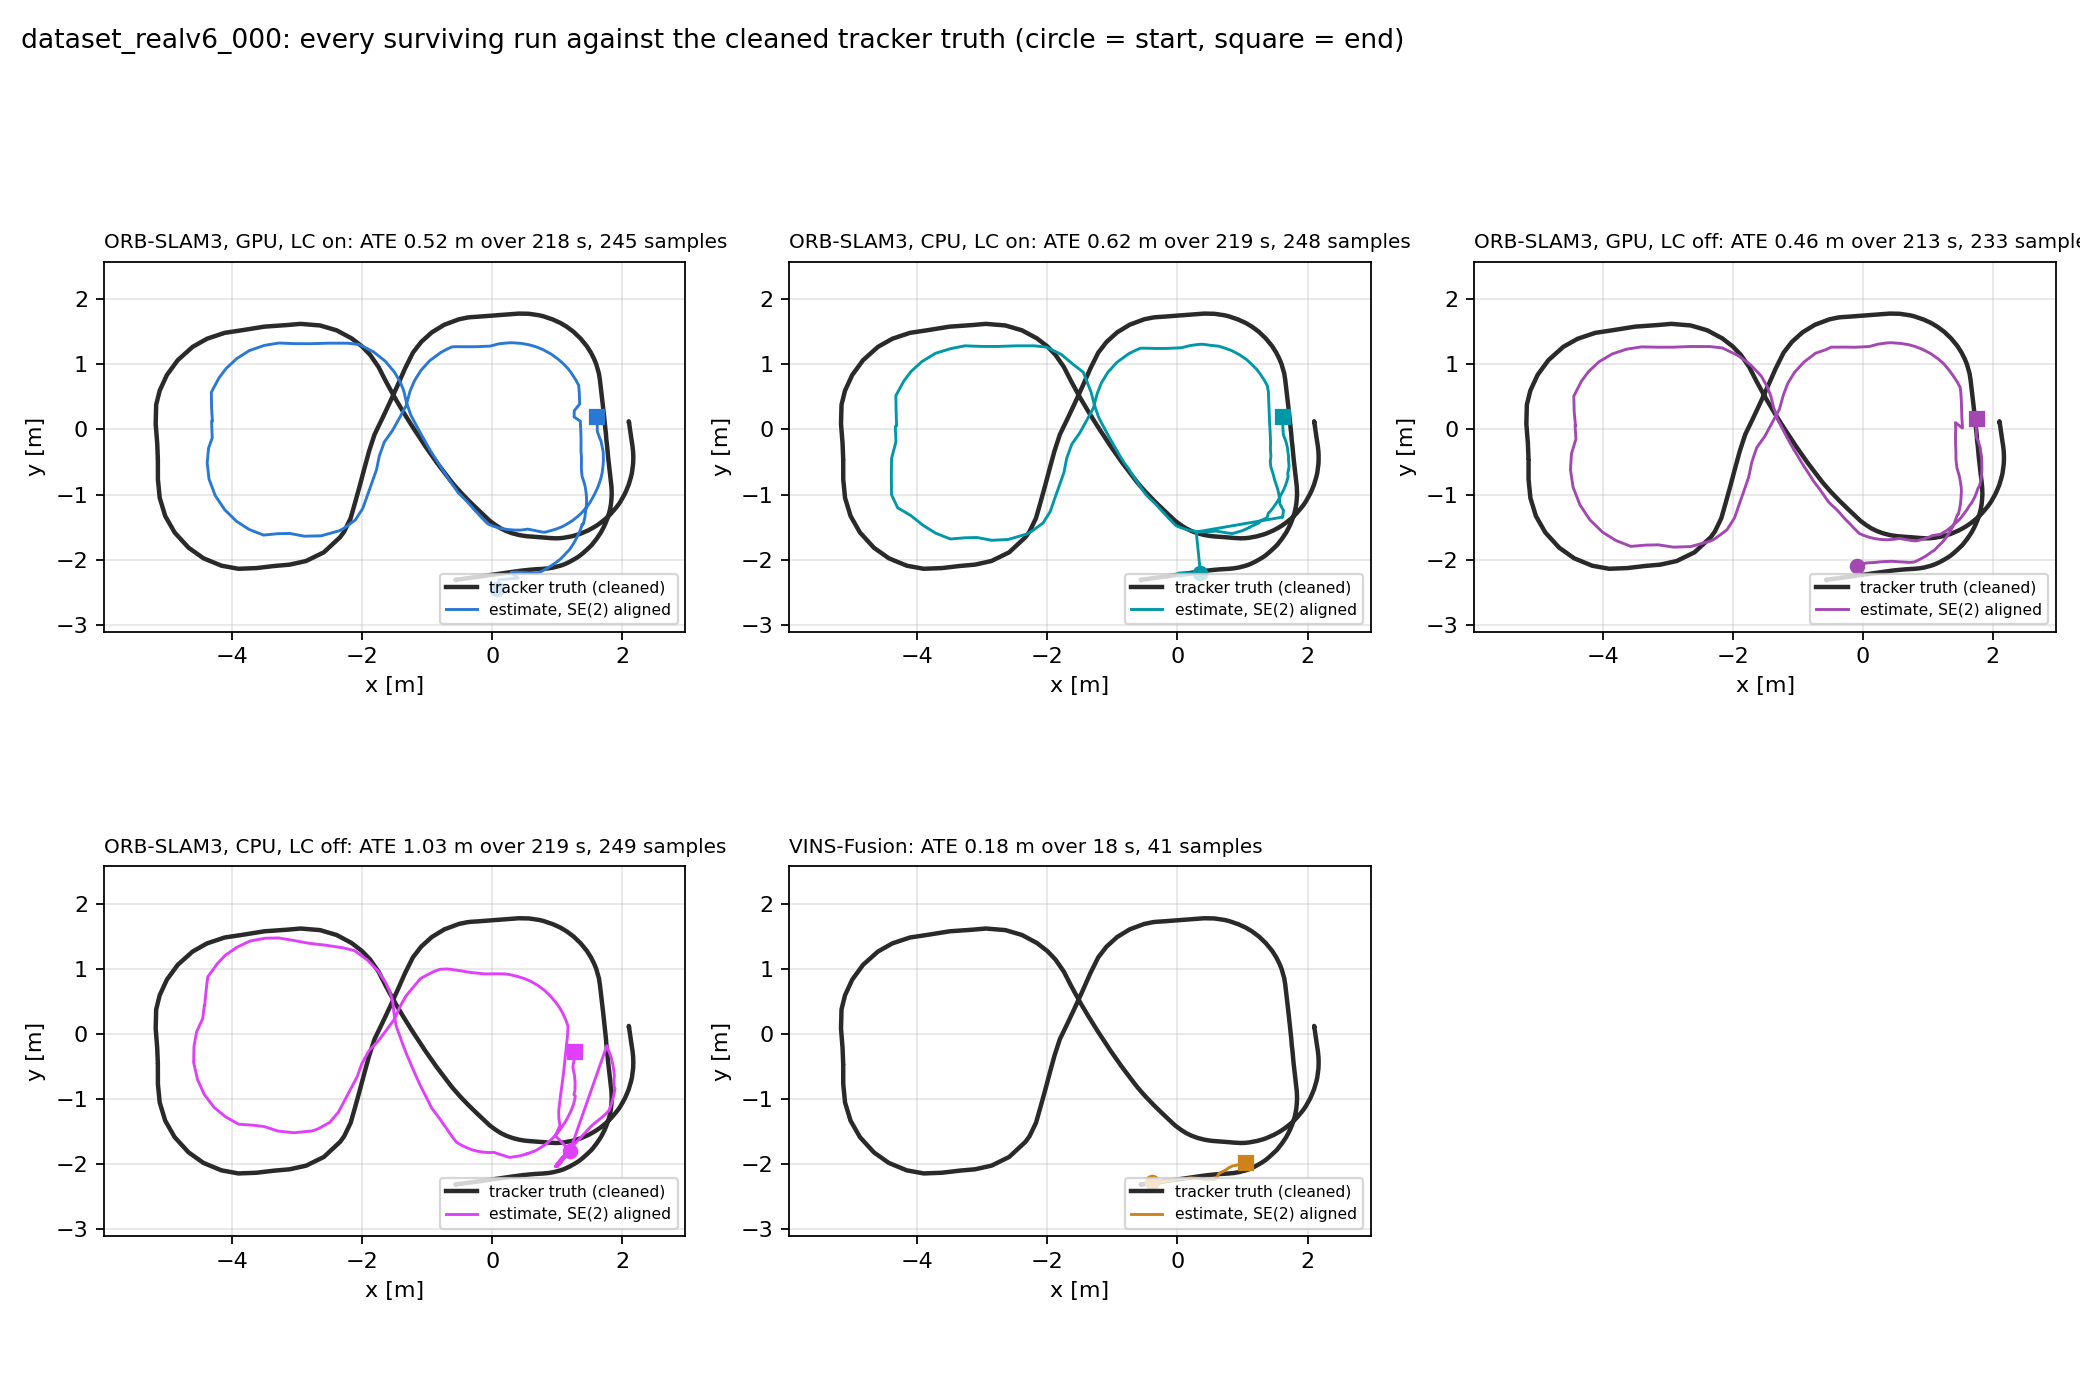
\includegraphics[width=\textwidth]{../../../../output/compare/real/realv6-insights/fig_paths_light.png}
  \caption[Real runs against the cleaned tracker truth.]{Every run against the
  cleaned tracker truth after rigid SE(2)
  alignment, one panel per run: ORB-SLAM3 with GPU or CPU extractor and loop
  closing on or off, and VINS-Fusion's \SI{18}{\second}.}
  \label{fig:realv6-paths}
\end{figure}

\begin{table}[htbp]
\centering
\small
\caption[Realv6: raw versus cleaned tracker export.]{The same ORB-SLAM3 run (GPU, LC on) scored against the tracker export as delivered and with one sample removed (the \SI{5.2}{\metre} excursion at \SI{184.9}{\second}). The time offsets are the values the wheel-speed cross-correlation found on each export on 2 November (peak correlation 0.10 raw, 0.61 cleaned), applied here as pinned values. The cleaned truth still fails the gap rule (66 gaps above \SI{1}{\second}, tracker at \SI{1.7}{\hertz}).}
\label{tab:realv6-cleaning}
\begin{tabular}{lrrrrr}
\toprule
Truth & GT path [m] & offset [s] & ATE [m] & median [m] & path ratio \\
\midrule
as delivered & 36.8 & 4.38 & 1.174 & 0.851 & 0.65 \\
one sample removed & 27.1 & -4.14 & 0.519 & 0.437 & 0.85 \\
\bottomrule
\end{tabular}
\end{table}


\paragraph{Analysis.} The front end is what separates the runs. The GPU
extractor drops a third to a half of the frames and holds \SI{0.5}{\metre}; the
CPU extractor drops two thirds and loses a factor of two, one of its runs with a
\SI{2}{\metre} vertical excursion the tool flags as implausible and the other
with three resets and a half-second of lost tracking. Loop closing changes
nothing that the front end does not change more. The remaining resets are an
initialisation effect, two or three \repo{local_mapping_bad_imu} map resets
inside the first \SI{13}{\second} and none after (zero in the GPU run without
loop closing); after them the error is a slow wave between \SI{0.05}{} and
\SI{1}{\metre}, not an accumulating drift (\cref{fig:realv6-orb}), and it does
not rise while turning in any run (\cref{tab:realv6-turning}). The estimates are
a uniform \SIrange{12}{15}{\percent} smaller than the tracker's path, which the
unmeasured lever arm, a stereo-baseline error or a tracker scale error could
each explain. One tracker sample decides the headline: scored against the
export as delivered, the GPU run reads \SI{1.17}{\metre} with a path ratio of
0.65, because that sample adds \SI{10}{\metre} of false path and dominates the
time alignment (\cref{tab:realv6-cleaning}).

\begin{figure}[htbp]
  \centering
  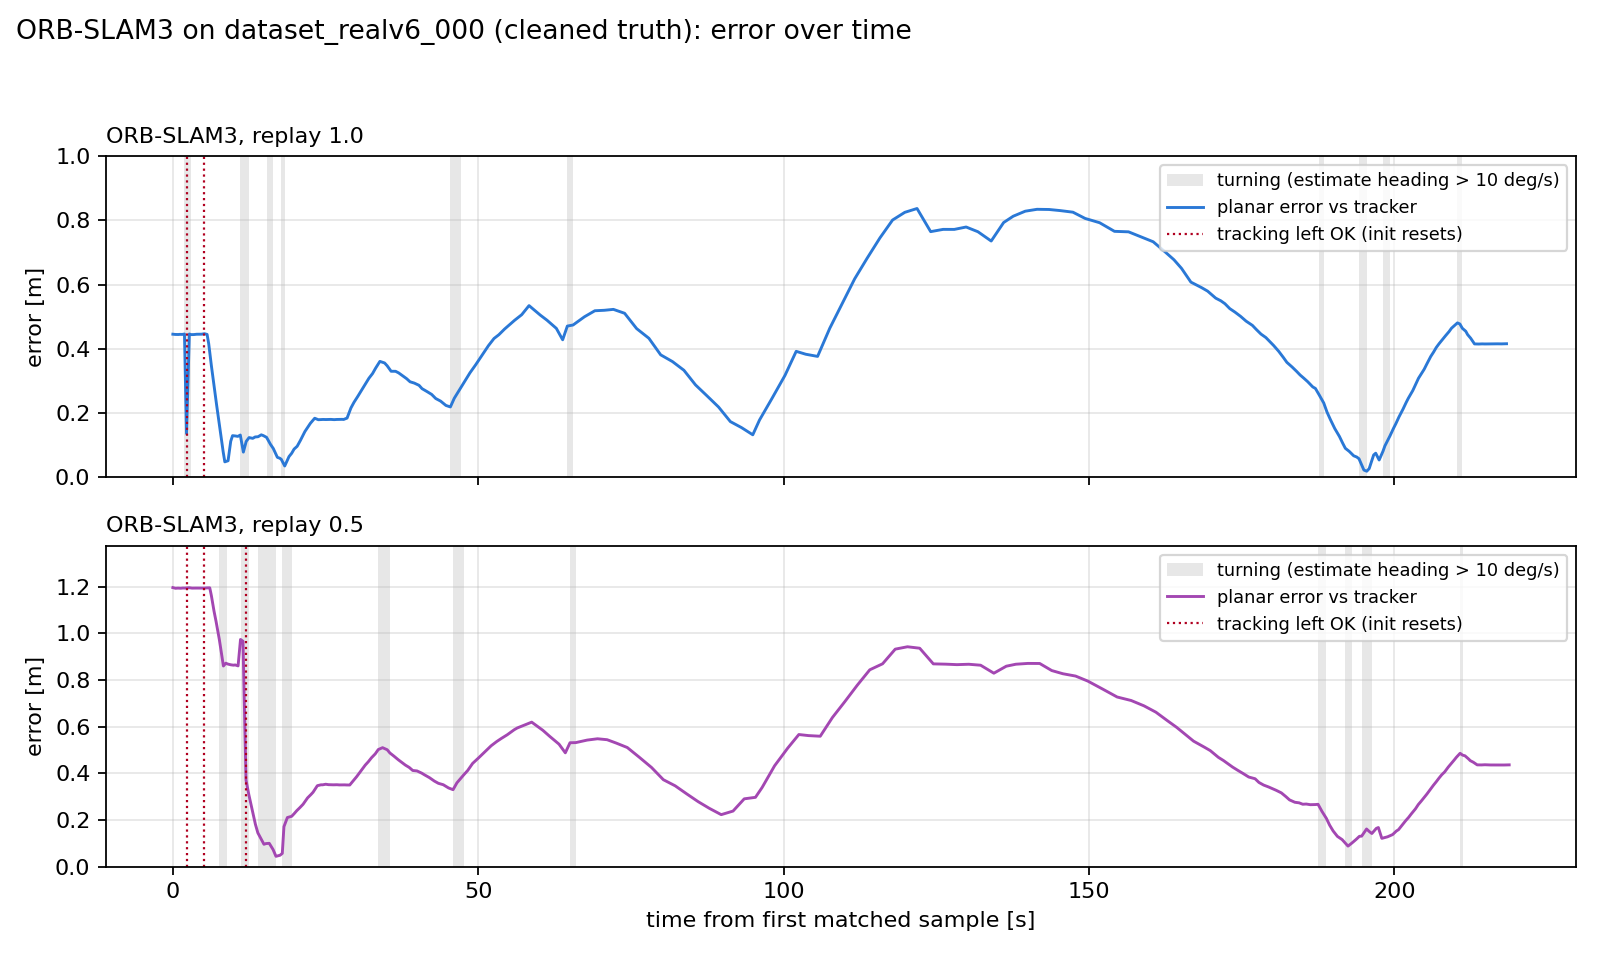
\includegraphics[width=\textwidth]{../../../../output/compare/real/realv6-insights/fig_orb_timeline_light.png}
  \caption[ORB-SLAM3 planar error over the run.]{ORB-SLAM3 planar error over
  the run, one panel per configuration;
  grey bands are turns, dotted red the initialisation resets.}
  \label{fig:realv6-orb}
\end{figure}

\begin{table}[htbp]
\centering
\small
\caption[Realv6: ORB-SLAM3 drift while turning versus on straights.]{ORB-SLAM3 on \repo{dataset_realv6_000}, cleaned truth: growth rate of the planar error while the aligned estimate's heading changes faster than \SI{10}{\degree\per\second} and on straights, with the time in each state. Positive = error growing. One run per configuration, so no test is possible.}
\label{tab:realv6-turning}
\begin{tabular}{lrrrr}
\toprule
Run & turning [mm/s] & straight [mm/s] & time turning [s] & time straight [s] \\
\midrule
ORB-SLAM3, GPU, LC on & -11.2 & -0.3 & 23 & 171 \\
ORB-SLAM3, CPU, LC on & -29.8 & -1.4 & 23 & 162 \\
ORB-SLAM3, GPU, LC off & 4.9 & -2.1 & 11 & 185 \\
ORB-SLAM3, CPU, LC off & -49.9 & -0.9 & 20 & 182 \\
\bottomrule
\end{tabular}
\end{table}


The setting was reached by elimination. With the IMU noise densities copied
from the VINS file the estimator was unstable on this recording, running away
in its velocity state at a different place in each run; six out-of-bounds reads
in the library were fixed without removing it, every other candidate was varied
without removing it, and raising the IMU noise densities tenfold removed it in
every run since. Those earlier runs were overwritten and carry no number here;
the search is in the ORB-SLAM3 engineering record.

VINS-Fusion's failure is a delivery defect. The node received 3\,187 of 6\,601
frames but used 6\,498 of the 43\,494 IMU messages it received, reset 217 times
on \repo{imu_gap}, and stopped after \SI{19}{\second}; behind that defect the
configuration still fixes a gravity norm of \num{9.2642} against the
\SI{9.878}{\metre\per\second\squared} this IMU reads at rest.

\begin{table}[htbp]
\centering
\small
\caption[Realv6: the VINS-Fusion run.]{VINS-Fusion on \repo{dataset_realv6_000}, 3 November 2026 (\repo{config/wil/stereo_imu.yaml}, IMU noise $\times 10$, gravity norm still \num{9.2642} against the \SI{9.878}{\metre\per\second\squared} this IMU reads at rest). The scored span is the \SI{18}{\second} it tracked before its last reset and is not a result.}
\label{tab:realv6-vins}
\begin{tabular}{lr}
\toprule
Quantity & Value \\
\midrule
camera frames received (bag: 6\,601) & 3187 \\
IMU messages received / samples used & 43494 / 6498 \\
\repo{imu_gap} resets & 217 \\
poses written / span of poses & 286 / \SI{19}{\second} \\
tracker samples matched & 41 of 43 in span \\
ATE over the tracked span & \SI{0.18}{\metre} (not a result) \\
\bottomrule
\end{tabular}
\end{table}


\begin{figure}[htbp]
  \centering
  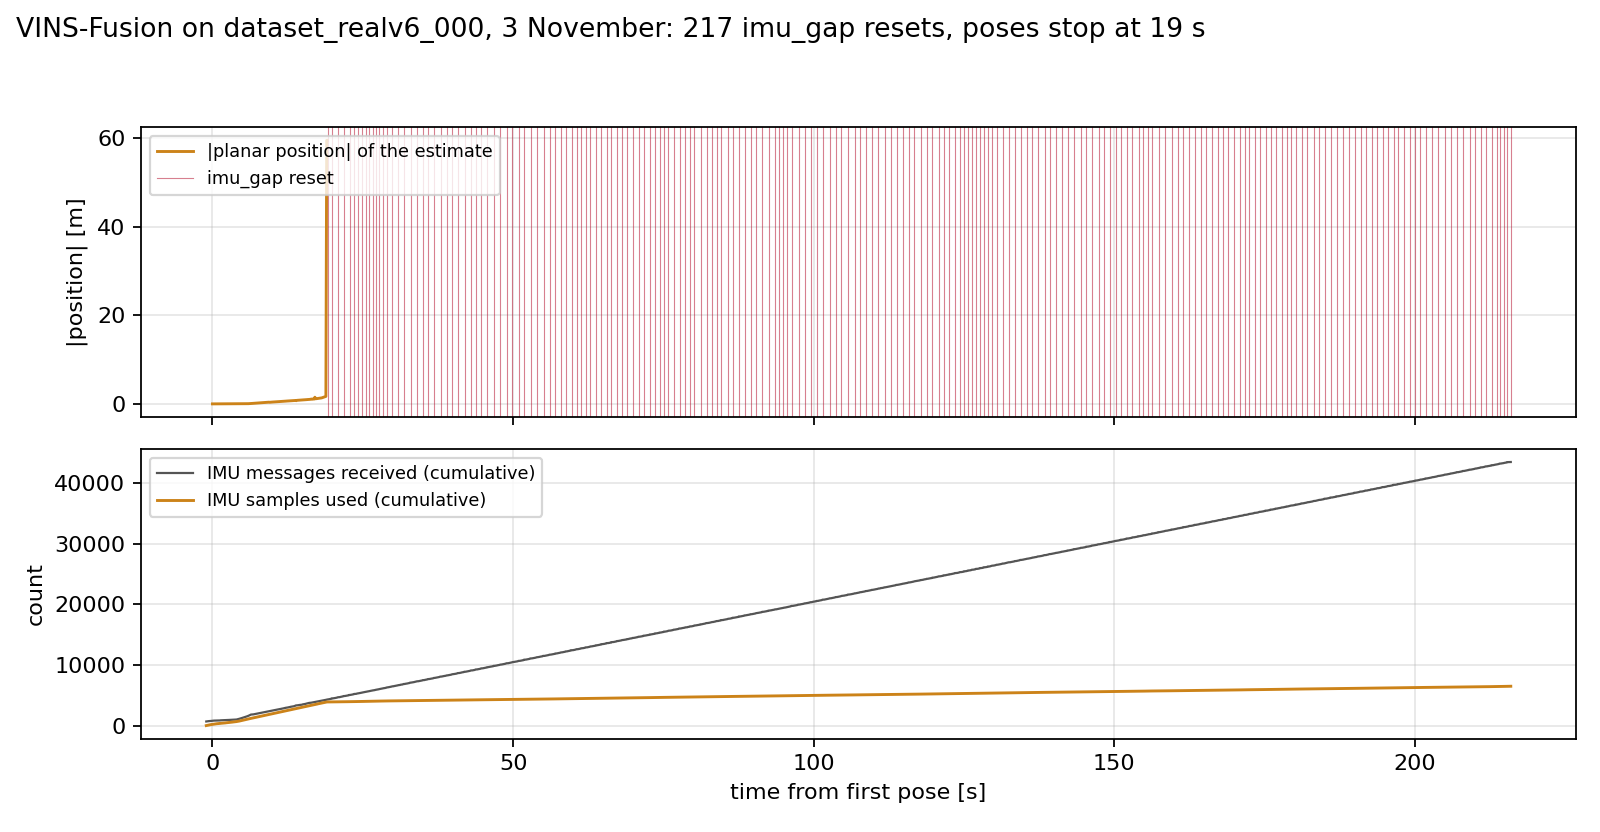
\includegraphics[width=\textwidth]{../../../../output/compare/real/realv6-insights/fig_vins_light.png}
  \caption[VINS-Fusion resets and IMU sample use.]{VINS-Fusion: distance from
  origin with every \repo{imu_gap} reset
  marked, and IMU messages received against samples used.}
  \label{fig:realv6-vins}
\end{figure}

\paragraph{Second recording set, realv7.} Three further recordings of 3 November
2026 (\repo{dataset_realv7_000}, \repo{_001}, \repo{_002}: \SI{21.6}{},
\SI{31.7}{} and \SI{23.4}{\metre} over \SI{97}{}, \SI{134}{} and
\SI{104}{\second}) have tracker exports that pass every validity rule
(\SIrange{5}{6}{\hertz}, no gap, no step). Each carries the same four ORB-SLAM3
configurations and one VINS-Fusion run. As written in the live log
(\cref{tab:realv7-tilt}, \cref{fig:realv7-tilt}), a plane fitted to the
ORB-SLAM3 estimate lies within \SI{10}{\degree} of horizontal in three runs of
twelve and at \SIrange{88}{90}{\degree} in five, every \repo{000} run among
them, with the plane normal exactly a body axis in every run; scored as
written, those nine runs are not scorable.

The per-frame diagnostics give the mechanism. The IMU initialised
\SIrange{3}{4}{\second} after the first pose. The upstream rule that resets a
map with less than \SI{2}{\centi\metre} between consecutive keyframes in the
first ten seconds after the initialisation then discarded it, the robot being
still at rest. The new map starts in the camera frame of the reset instant, and
in it the re-initialisation was starved: upstream attempts it only with an
empty keyframe queue, which a keyframe every \SI{0.25}{\second} and
\SI{250}{\milli\second} of map-point creation per keyframe never allowed. The
IMU re-initialised after \SIrange{37}{92}{\second} in seven runs, never in two,
and early (\SI{6.7}{\second}) in the one run that was level. Until then the
estimate is stereo-only in a map whose vertical is the camera's $y$ axis, and
the late re-initialisation rotates the map under the already-written poses (the
\SIrange{1.9}{6.8}{\metre} steps).

A scorer-side repair was written while the cause was being found: it rotates
the pre-initialisation poses by the rotation measured at the initialisation
frame and levels each map's fitted plane, both without using the truth.
It is kept for the record and is not used
for any result below, because the defect it worked around is now fixed in the
estimator; the one figure it produced that is still worth quoting is that on
\repo{000} it recovered \SIrange{0.252}{0.275}{\metre} from runs whose
estimates were lying on their side.

The fork's patch 15 adds two switches that attempt the initialisation with a
queued backlog and skip the low-motion reset for stereo. On 11 November 2026
all twelve runs were re-made with both active, and
\cref{tab:realv7-patch15} reports them scored \emph{raw}: neither of the two
repairs above was applied, which is the point of the table.

The upstream behaviour is gone from every run. The IMU initialised at
\SIrange{2.8}{4.7}{\second} and was retained; thirteen of the sixteen request
no map reset at all and the other three request one for a timestamp jump, not
for insufficient motion. The plane of the estimate now lies
\SIrange{0.2}{2.8}{\degree} from horizontal in every run against the
\SIrange{5}{90}{\degree} of \cref{tab:realv7-tilt}, and the vertical range
falls from as much as \SI{9.6}{} to at most \SI{1.00}{\metre}. Under the
scorer's own rules seven \repo{realv7} runs are now \status{completed} where
none was before and the other five are \status{partial}; the four
\repo{realv6} runs remain rejected, not for anything the estimator did but
because that recording's tracker export fails the validity rules.

The accuracy claim is narrower than the defect claim, and the three recordings
disagree. Set against the same configuration under upstream initialisation
\emph{after both repairs} --- each estimator at the best obtainable from it ---
patch 15 matches it on \repo{realv7_000} (\SIrange{0.251}{0.268}{} against
\SIrange{0.252}{0.275}{\metre}), is mixed on \repo{_001}, where two runs
improve and two worsen and one of those reaches \SI{1.278}{} against
\SI{0.817}{\metre}, and beats it on \repo{_002}
(\SIrange{0.172}{0.198}{} against \SIrange{0.472}{2.115}{\metre}, every one
of the four better than anything the repair obtained there) and on
\repo{realv6_000}, where all four improve
(\SIrange{0.404}{0.480}{} against \SIrange{0.457}{1.028}{\metre}) and the two
CPU runs improve most. The
defensible statement is therefore not that patch 15 is more accurate. It is
that patch 15 removes the need for the repair: it reaches on the raw estimate
what the stock estimator reaches only after its frame bookkeeping has been
corrected offline, and on the one recording the repair handled worst it
reaches considerably more. The
\SIrange{0.172}{0.198}{\metre} runs of \repo{_002} are the most accurate
real-robot ORB-SLAM3 figures in this report.

\begin{queried}[Open: what the improvement is owed to]
Two things differ between the two sets of runs, not one. Patch 15 is the
first; the second is that \repo{IMU.NoiseGyro} and \repo{IMU.NoiseAcc} were
inflated tenfold on 3 November, and no artefact records which values that
afternoon's runs used, because \repo{run_metadata.csv} stores the
configuration's path and not its contents. The loss of the tilt is
patch 15's: the upstream rule tests keyframe spacing below \SI{2}{\centi\metre}
within \SI{10}{\second} and cannot be influenced by an inertial noise density.
Any part of the accuracy difference is not separable on the present evidence.
One control run, the same bag at today's noise with both switches returned to
upstream, would separate them and has not been made.
\end{queried}

\begin{queried}[Provenance: the 3 November estimates are gone]
The re-runs overwrote \path{output/output_orb/real/dataset_realv7_00*/} in
place, so the pre-patch-15 estimates of all three recordings no longer exist
and neither \cref{tab:realv7-tilt} nor \cref{fig:realv7-tilt} can be
regenerated; the frozen copies beside the generator are the only record of the
behaviour this section reports as corrected. A run directory should be
written under a name that carries its configuration, so that a re-run cannot
overwrite the evidence for the behaviour it replaces.
\end{queried} VINS-Fusion
diverges on all three with the IMU stream intact (zero resets) and
\SIrange{40}{45}{\percent} of the frames received (\cref{tab:realv7-vins}); its
gravity norm has since been set to the measured \SI{9.886}{\metre\per\second\squared}.

% FROZEN 11 Nov 2026: the realv7_002 run directories this was computed from were
% overwritten by the patch-15 re-runs the same day, so realv7_002 CANNOT be
% regenerated. Do not replace this file from script/realv7_insights.py.
\begin{table}[htbp]
\centering
\scriptsize\setlength{\tabcolsep}{3pt}
\caption[Evidence of the initialisation defect: the plane of every estimate under stock ORB-SLAM3.]{ORB-SLAM3 on the three \repo{dataset_realv7} recordings, 3 November 2026 afternoon, same setting as the realv6 runs: the plane of each estimate as written in the live log, before any repair. ``Tilt'' is the angle between the plane fitted to the estimate's 3-D positions and the horizontal; ``off-plane'' the rms distance of the positions from that plane. A floor robot's estimate should be horizontal: a tilt near \SI{90}{\degree} means the poses were written while the map was not gravity-aligned (IMU not initialised; the vertical is then the camera's $y$ axis). The scores are in the patched runs of the real-robot results table.}
\label{tab:realv7-tilt}
\begin{tabular}{llrrrr}
\toprule
Recording & Run & tilt [\si{\degree}] & off-plane [m] & z range [m] & resets \\
\midrule
\repo{realv7_000} & GPU, LC on & \textcolor{flagred}{89.1} & 0.35 & 6.87 & 3 s \\
\repo{realv7_000} & GPU, LC off & \textcolor{flagred}{89.5} & 0.02 & 6.98 & 3 s \\
\repo{realv7_000} & CPU, LC on & \textcolor{flagred}{88.8} & 0.41 & 6.88 & 5 s \\
\repo{realv7_000} & CPU, LC off & \textcolor{flagred}{87.9} & 0.58 & 6.79 & 4 s \\
\addlinespace
\repo{realv7_001} & GPU, LC on & \textcolor{flagred}{88.8} & 0.05 & 9.64 & 4 s \\
\repo{realv7_001} & GPU, LC off & 6.1 & 1.12 & 5.77 & 3 s, 5 s \\
\repo{realv7_001} & CPU, LC on & 1.5 & 0.07 & 0.38 & 4 s \\
\repo{realv7_001} & CPU, LC off & \textcolor{flagred}{13.0} & 1.05 & 5.23 & 5 s \\
\addlinespace
\repo{realv7_002} & GPU, LC on & \textcolor{flagred}{37.7} & 0.87 & 4.08 & 3 s, 49 s, 59 s \\
\repo{realv7_002} & GPU, LC off & \textcolor{flagred}{59.7} & 0.83 & 4.80 & 49 s \\
\repo{realv7_002} & CPU, LC on & 5.2 & 0.73 & 2.94 & none \\
\repo{realv7_002} & CPU, LC off & \textcolor{flagred}{21.7} & 0.84 & 7.03 & none \\
\bottomrule
\end{tabular}
\end{table}


\begin{figure}[p]
  \centering
  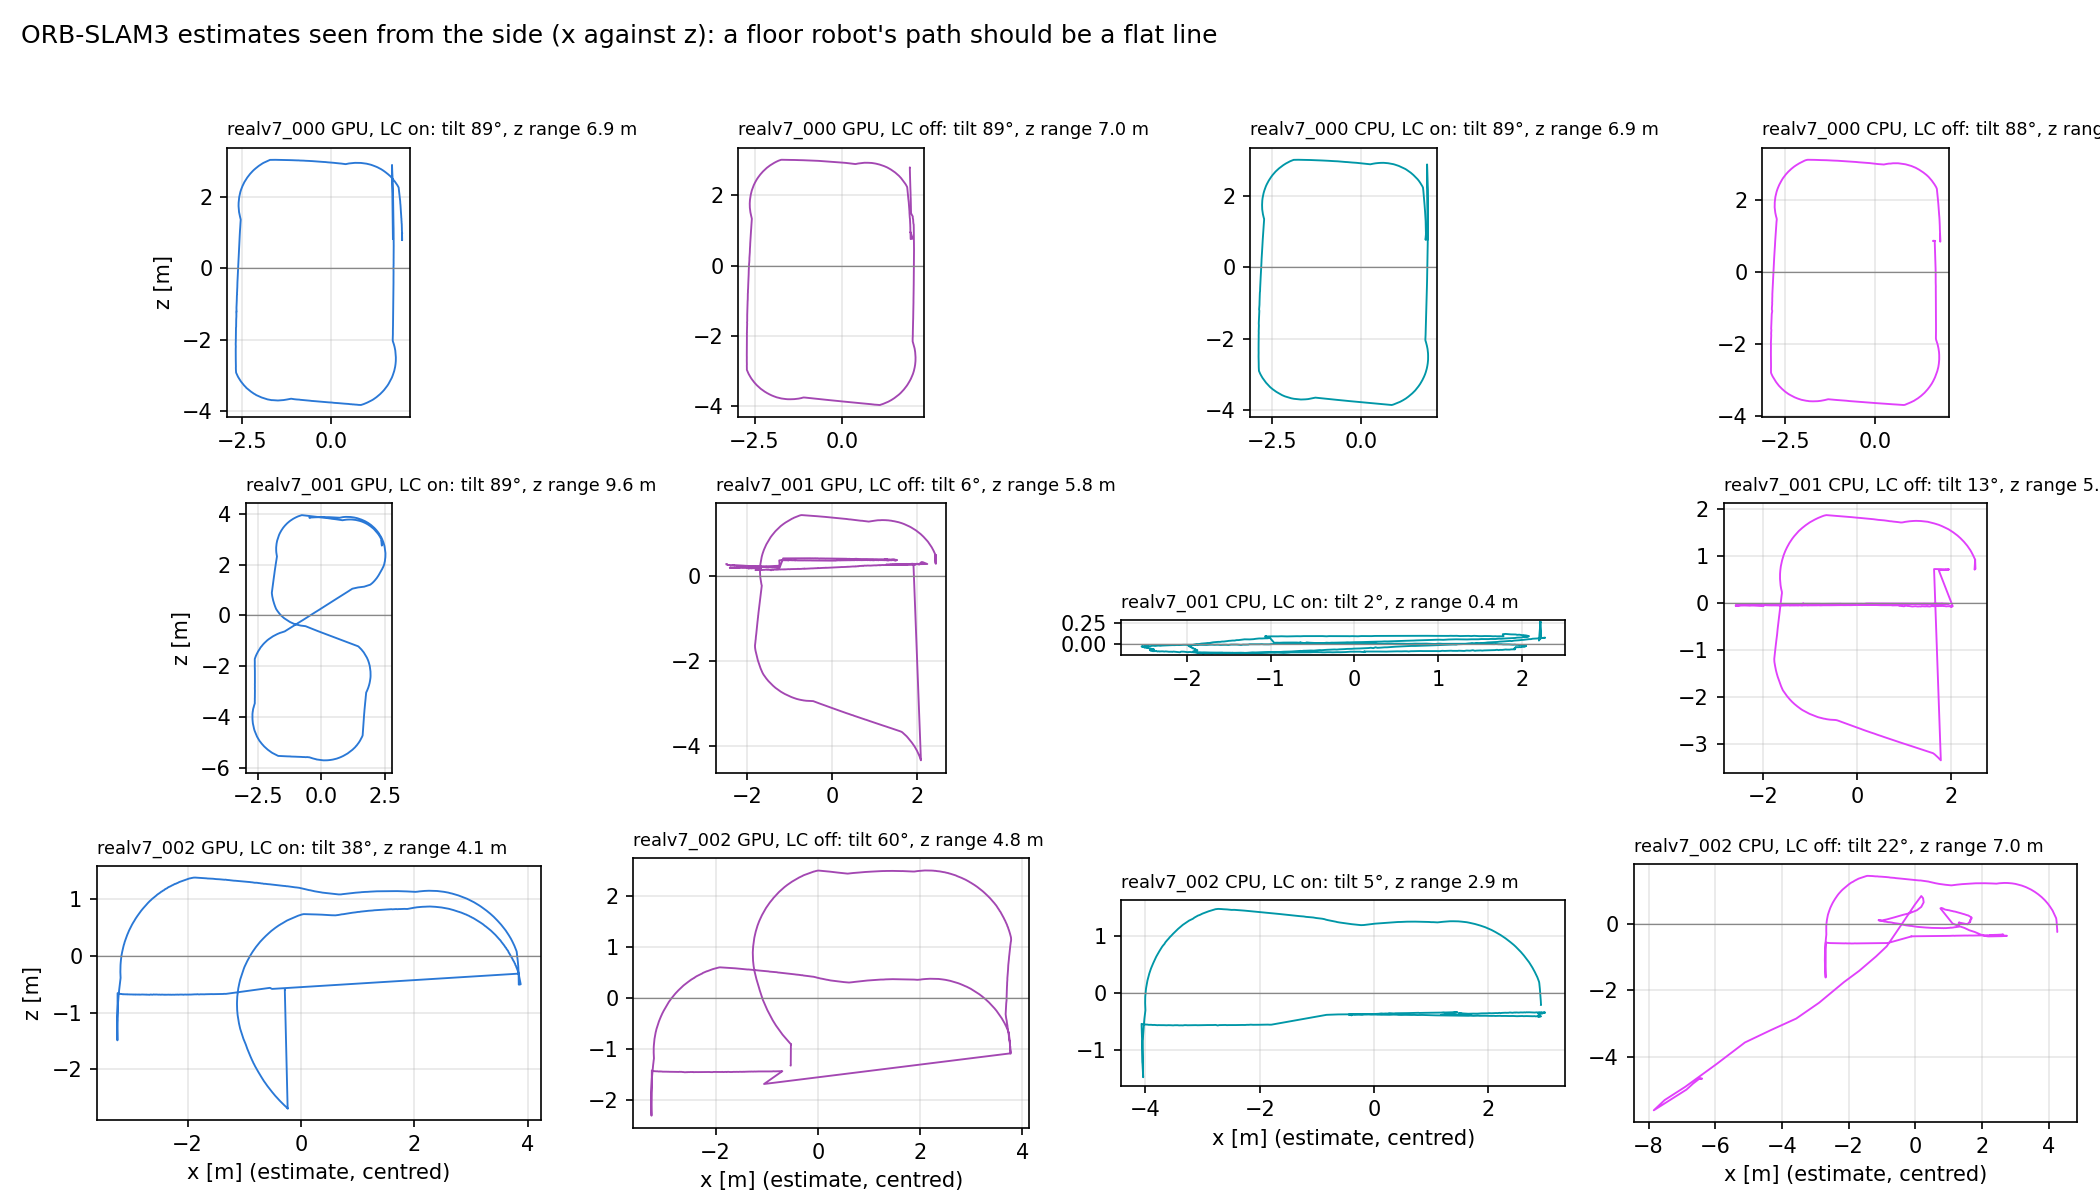
\includegraphics[width=\textwidth]{../../../../output/compare/real/realv7-insights/fig_tilt_light_prepatch15.png}
  \caption[The twelve realv7 estimates as written in the live log.]{The twelve
  \repo{realv7} ORB-SLAM3 estimates as written in the live
  log, seen from the side ($x$ against $z$, centred); a floor robot's path should
  be a flat line. This is the defect that fork patch 15 removes; the estimates
  it produces instead are \cref{fig:realv7-paths-patch15}.}
  \label{fig:realv7-tilt}
\end{figure}

% Generated by script/realv7_patch15.py -- do not edit by hand.
\begin{table}[htbp]
\centering
\caption[Every real-robot run, with the upstream initialisation defect patched out.]{Every real-robot ORB-SLAM3 run on the four recordings that carry an independent planar reference, with fork patch 15 active (\repo{LocalMapping.resetOnLowMotion} 0, \repo{LocalMapping.initWithBacklog} 1) and scored \emph{raw}: neither \texttt{--join-imu-init} nor \texttt{--level-plane}, the repairs every other \repo{realv7} figure in this chapter depends on. ``Tilt'' and ``z range'' are measured the same way as in \cref{tab:realv7-tilt}, so the two are comparable. ``ATE before'' is the same configuration on the same recording on 3 November, scored raw. Front-end identity was confirmed from the median tracking latency (GPU \SIrange{41}{50}{\milli\second}, CPU \SIrange{104}{113}{\milli\second}), not from the run name. ``Stock + repair'' is the same configuration on the same recording on 3 November, under upstream initialisation and, for \repo{realv7}, only after the scorer-side frame repair that has since been retired: it is the fair comparison, each estimator at the best obtainable from it. For \repo{realv6_000}, which never showed the tilt and needed no repair, ``before'' is the same run scored against the same cleaned tracker export without the switches. Status is the scorer's: it rejects a run whose estimate spans more than \SI{1}{\metre} vertically, and it rejects every \repo{realv6} run because that recording's tracker export is \SI{1.7}{\hertz} and fails the validity rules written for the \SI{7}{\hertz} one, so its rows are diagnostics. Lever arm still unmeasured, so every value is provisional.}
\label{tab:realv7-patch15}
\small
\resizebox{\textwidth}{!}{%
\begin{tabular}{llrrr rr rrl}
\toprule
Recording & Run & IMU init [\si{\second}] & resets & tilt [\si{\degree}] & z range [\si{\metre}] & Kept & ATE [\si{\metre}] & Before [\si{\metre}] & status \\
\midrule
\repo{realv6_000} & GPU, LC on & 3.1 & 0 & 1.1 & 0.27 & 0.58 & 0.478 & 0.519 & failed \\
 & GPU, LC off & 4.5 & 1 & 1.2 & 0.33 & 0.51 & 0.404 & 0.457 & failed \\
 & CPU, LC on & 3.0 & 0 & 0.2 & 0.31 & 0.30 & 0.480 & 0.618 & failed \\
 & CPU, LC off & 2.8 & 0 & 1.8 & 0.36 & 0.28 & 0.456 & 1.028 & failed \\
\addlinespace
\repo{realv7_000} & GPU, LC on & 3.0 & 0 & 2.1 & 0.37 & 0.75 & 0.268 & 0.252 & partial \\
 & GPU, LC off & 3.0 & 0 & 2.0 & 0.36 & 0.69 & 0.251 & 0.259 & partial \\
 & CPU, LC on & 4.3 & 1 & 2.6 & 0.39 & 0.34 & 0.266 & 0.275 & partial \\
 & CPU, LC off & 4.3 & 1 & 1.6 & 0.34 & 0.32 & 0.259 & 0.261 & partial \\
\addlinespace
\repo{realv7_001} & GPU, LC on & 2.9 & 0 & 2.0 & 0.42 & 0.71 & 0.451 & 0.477 & completed \\
 & GPU, LC off & 4.7 & 0 & 1.7 & 0.45 & 0.67 & 1.278 & 0.817 & completed \\
 & CPU, LC on & 2.8 & 0 & 0.8 & 0.40 & 0.33 & 0.575 & 0.438 & completed \\
 & CPU, LC off & 2.9 & 0 & 2.0 & 0.42 & 0.32 & 0.442 & 0.558 & completed \\
\addlinespace
\repo{realv7_002} & GPU, LC on & 3.0 & 0 & 2.0 & 0.43 & 0.57 & 0.172 & 2.115 & completed \\
 & GPU, LC off & 3.1 & 0 & 2.5 & 0.45 & 0.63 & 0.198 & 2.079 & partial \\
 & CPU, LC on & 3.2 & 0 & 2.5 & 0.87 & 0.32 & 0.194 & 0.472 & completed \\
 & CPU, LC off & 3.2 & 0 & 2.8 & 1.00 & 0.31 & 0.198 & 1.675 & completed \\
\bottomrule
\end{tabular}}
\end{table}


\begin{figure}[p]
  \centering
  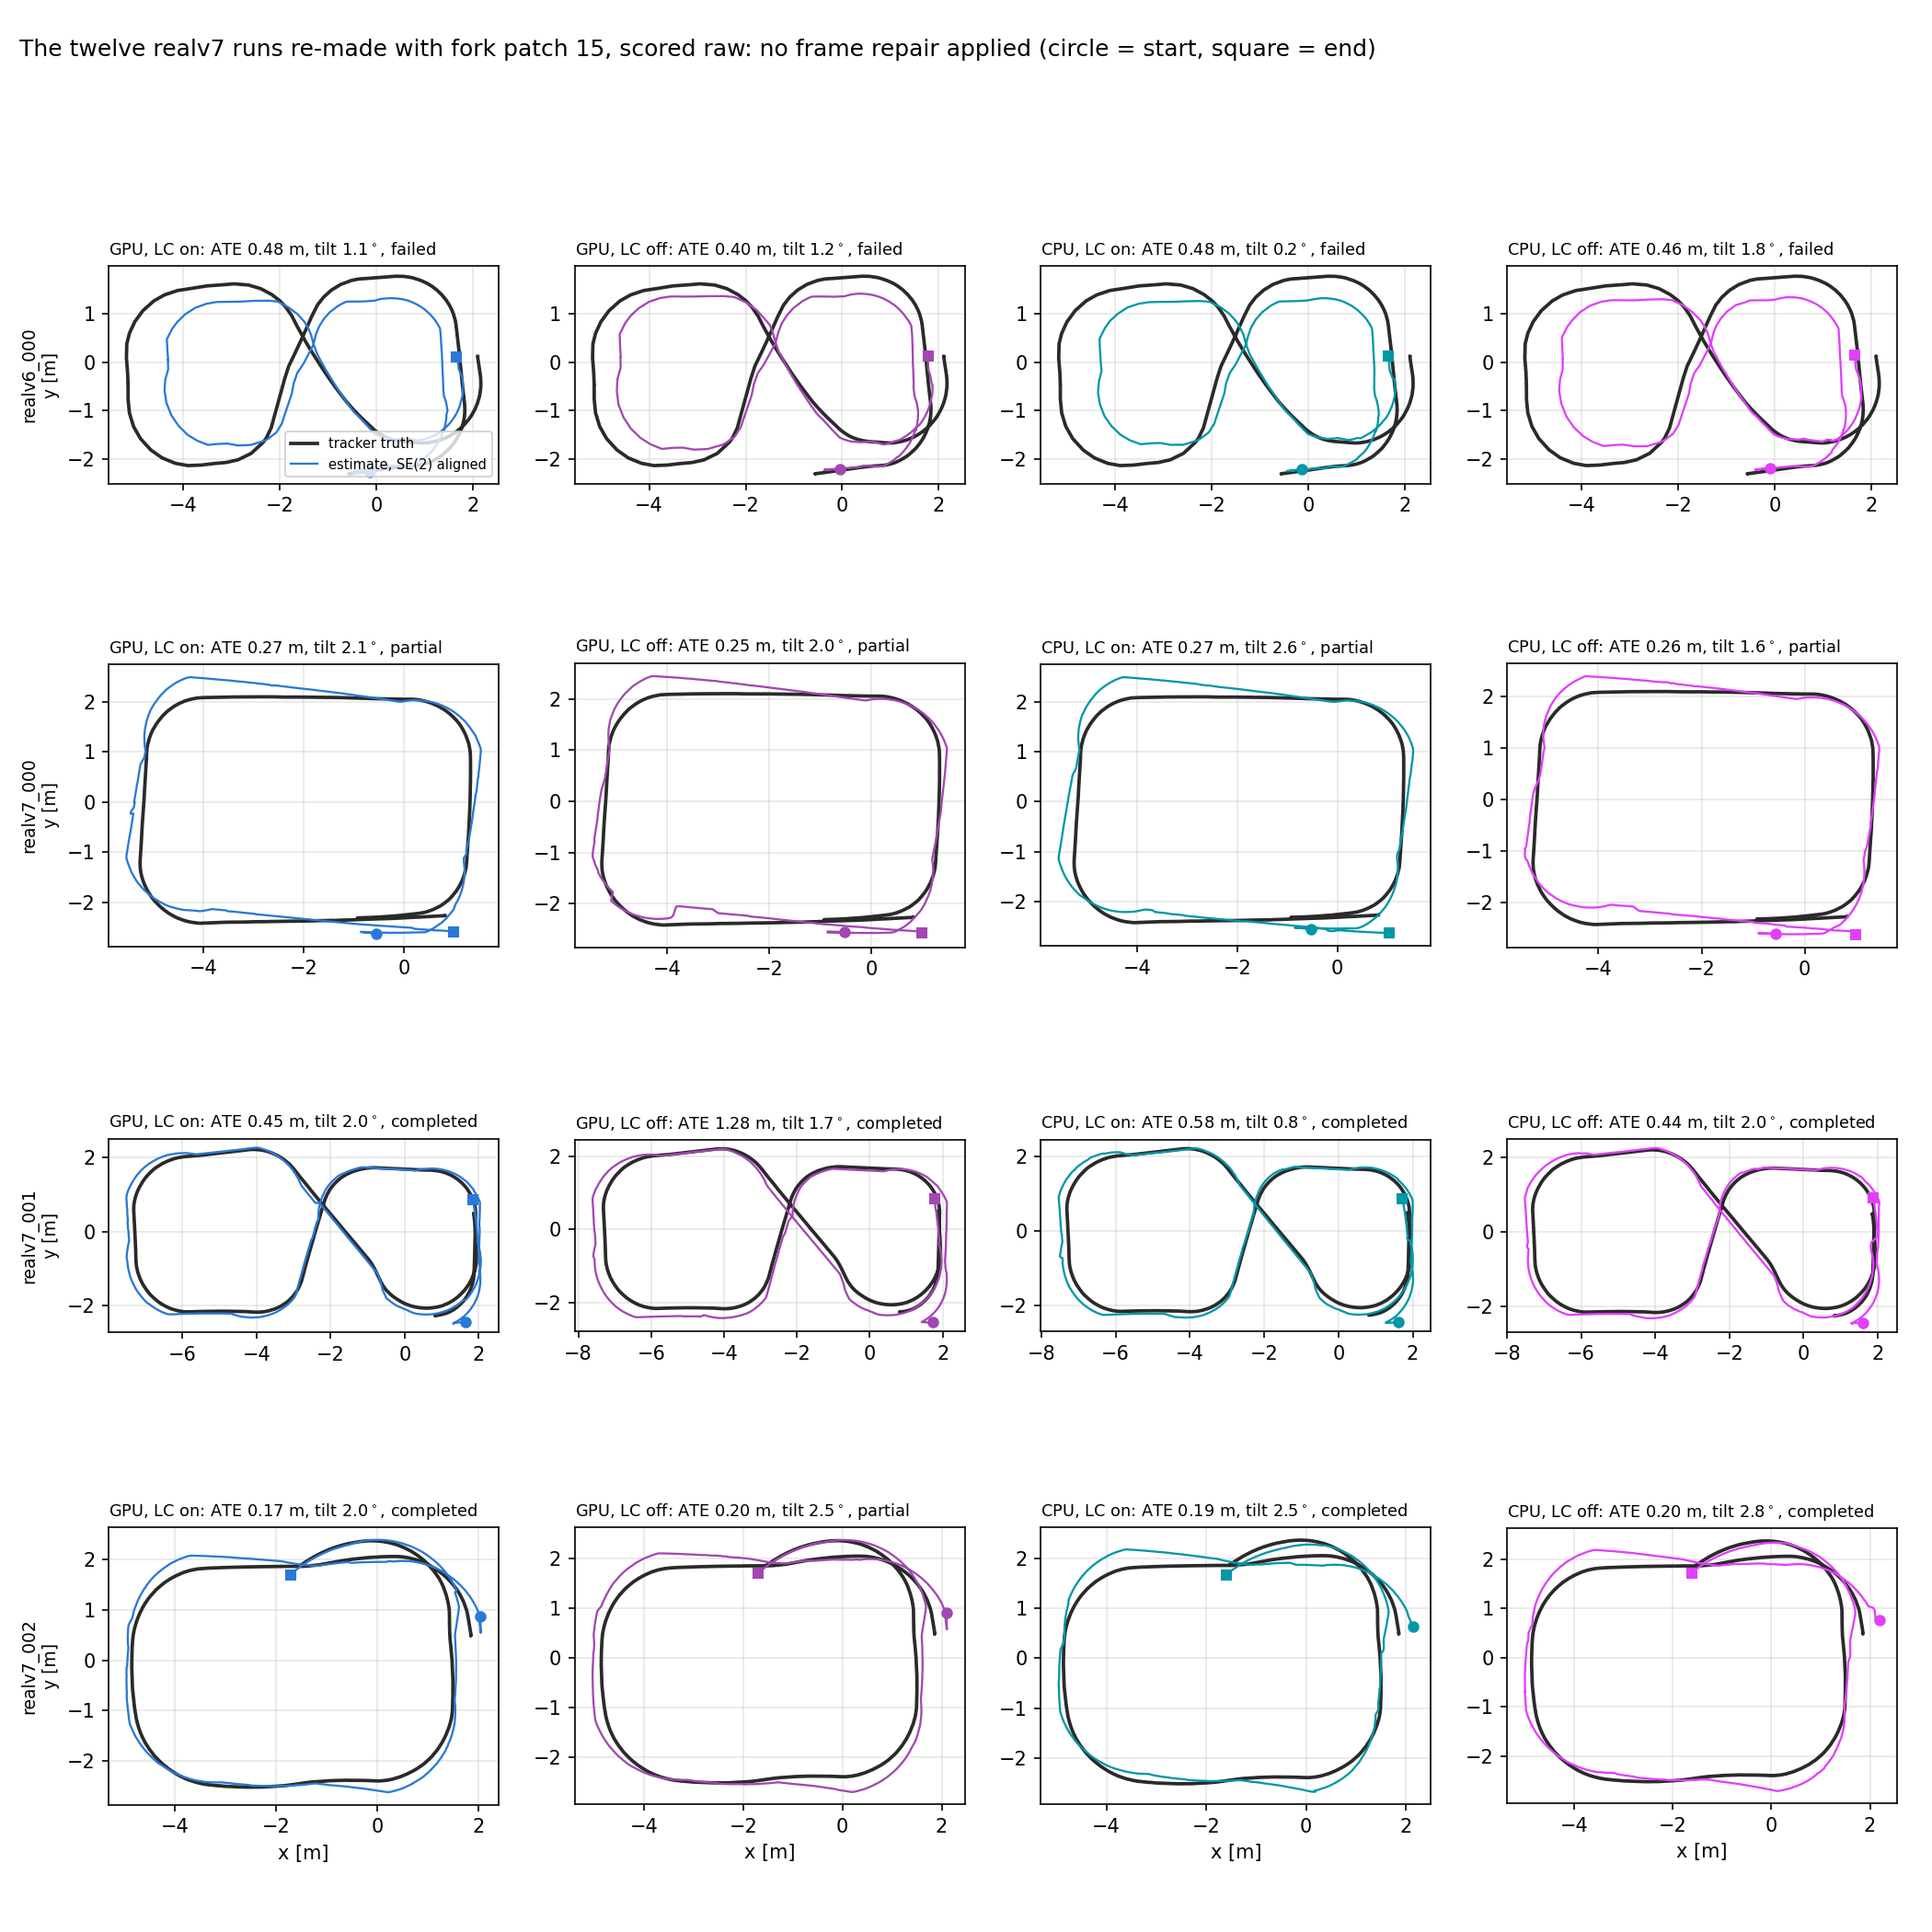
\includegraphics[width=\textwidth]{../../../../output/compare/real/realv7-insights/fig_paths_patch15_light.png}
  \caption[Every real-robot run with patch 15, scored raw.]{Every real-robot
  ORB-SLAM3 run on the four recordings that carry an independent planar
  reference, with fork patch 15 active, against the tracker truth after rigid
  SE(2) alignment. No repair of
  any kind is applied: these are the estimates as the node wrote them, where
  those of \cref{fig:realv7-tilt} had to be levelled and rotated before they
  could be drawn at all. Each panel gives the planar ATE, the tilt of the
  fitted plane and the scorer's status.}
  \label{fig:realv7-paths-patch15}
\end{figure}

\begin{table}[htbp]
\centering
\small
\caption[Realv7: the VINS-Fusion runs.]{VINS-Fusion on the three \repo{dataset_realv7} recordings (\repo{config/wil/stereo_imu.yaml}, IMU noise $\times 10$, gravity norm \num{9.2642}). Frames received against the bag's count (\SI{30}{\hertz} over the recording), IMU use, resets, and where the estimate ended.}
\label{tab:realv7-vins}
\resizebox{\textwidth}{!}{%
\begin{tabular}{lrrrrr}
\toprule
Recording & frames received & IMU received / used & resets & z range [m] & $|p|$ at end [m] \\
\midrule
\repo{realv7_000} & 1155 of about 2663 & 17906 / 19053 & 0 & 12834403 & 37554 \\
\repo{realv7_001} & 1541 of about 3686 & 24809 / 26340 & 0 & 3701 & 15974 \\
\repo{realv7_002} & 1271 of about 2910 & 19368 / 20627 & 0 & 25937 & 5252 \\
\bottomrule
\end{tabular}}
\end{table}


\begin{queried}[Sparse reference]
The tracker ran at \SI{1.7}{\hertz} rather than its nominal \SI{7}{\hertz} on
\repo{realv6}, and
the validity rules were written for the faster export. Either the export has to
be re-captured at full rate or a rule for sparse references has to be written
before any value from this recording is quoted outside a diagnostic.
\end{queried}

\paragraph{Summary.} On the four real recordings the two families are in the
same accuracy class. Wheel+gyro dead reckoning, with one constant fitted on
\repo{realv7_000} and held, localises the robot to \SI{0.26}{} and
\SI{0.22}{\metre} on the other two \repo{realv7} recordings and
\SI{0.46}{\metre} on \repo{realv6}; ORB-SLAM3, with the upstream
initialisation defect patched out and scored raw, reads \SI{0.44}{},
\SI{0.17}{} and \SI{0.40}{\metre} on the same three. The baseline leads on
one, ties on one and is beaten on the third. The cause of the IMU staying
uninitialised for most of nine of the original twelve \repo{realv7} runs ---
an upstream map reset at the initialisation and a starved re-initialisation
--- is diagnosed, patched in the fork and now exercised on every run; what the
patch is shown to do is remove the need for the scorer's frame repair, not to
improve accuracy, which it matches on one recording, splits on a second and
improves on the other two. VINS-Fusion has no valid run on any recording,
through two delivery and configuration defects that are diagnosed and in part
corrected. The marker-to-IMU lever arm is unmeasured, so every figure here is
provisional, and \repo{realv6}'s tracker export fails the validity rules
written for the faster one, so its rows are diagnostics.

\textbf{Next action.} Run one \repo{realv7} recording with both initialisation
switches returned to upstream at the current inertial noise, which is the
control that separates patch 15 from the tenfold noise change made the same
week; re-run VINS-Fusion with the corrected gravity norm; measure the
marker-to-IMU lever arm, which every real figure in this chapter is
provisional on; and replace the fitted wheel-speed constant with a measured
one. Write each run under a directory name that carries its configuration, so
that no re-run overwrites the evidence it replaces.

% =====================================================================
\FloatBarrier

\end{document}
